\documentclass[]{book}
\usepackage{lmodern}
\usepackage{amssymb,amsmath}
\usepackage{ifxetex,ifluatex}
\usepackage{fixltx2e} % provides \textsubscript
\ifnum 0\ifxetex 1\fi\ifluatex 1\fi=0 % if pdftex
  \usepackage[T1]{fontenc}
  \usepackage[utf8]{inputenc}
\else % if luatex or xelatex
  \ifxetex
    \usepackage{mathspec}
  \else
    \usepackage{fontspec}
  \fi
  \defaultfontfeatures{Ligatures=TeX,Scale=MatchLowercase}
\fi
% use upquote if available, for straight quotes in verbatim environments
\IfFileExists{upquote.sty}{\usepackage{upquote}}{}
% use microtype if available
\IfFileExists{microtype.sty}{%
\usepackage{microtype}
\UseMicrotypeSet[protrusion]{basicmath} % disable protrusion for tt fonts
}{}
\usepackage[margin=1in]{geometry}
\usepackage{hyperref}
\hypersetup{unicode=true,
            pdftitle={DALEX: Descriptive mAchine Learning EXplanations},
            pdfauthor={MI2DataLab},
            pdfborder={0 0 0},
            breaklinks=true}
\urlstyle{same}  % don't use monospace font for urls
\usepackage{natbib}
\bibliographystyle{apalike}
\usepackage{color}
\usepackage{fancyvrb}
\newcommand{\VerbBar}{|}
\newcommand{\VERB}{\Verb[commandchars=\\\{\}]}
\DefineVerbatimEnvironment{Highlighting}{Verbatim}{commandchars=\\\{\}}
% Add ',fontsize=\small' for more characters per line
\usepackage{framed}
\definecolor{shadecolor}{RGB}{248,248,248}
\newenvironment{Shaded}{\begin{snugshade}}{\end{snugshade}}
\newcommand{\KeywordTok}[1]{\textcolor[rgb]{0.13,0.29,0.53}{\textbf{#1}}}
\newcommand{\DataTypeTok}[1]{\textcolor[rgb]{0.13,0.29,0.53}{#1}}
\newcommand{\DecValTok}[1]{\textcolor[rgb]{0.00,0.00,0.81}{#1}}
\newcommand{\BaseNTok}[1]{\textcolor[rgb]{0.00,0.00,0.81}{#1}}
\newcommand{\FloatTok}[1]{\textcolor[rgb]{0.00,0.00,0.81}{#1}}
\newcommand{\ConstantTok}[1]{\textcolor[rgb]{0.00,0.00,0.00}{#1}}
\newcommand{\CharTok}[1]{\textcolor[rgb]{0.31,0.60,0.02}{#1}}
\newcommand{\SpecialCharTok}[1]{\textcolor[rgb]{0.00,0.00,0.00}{#1}}
\newcommand{\StringTok}[1]{\textcolor[rgb]{0.31,0.60,0.02}{#1}}
\newcommand{\VerbatimStringTok}[1]{\textcolor[rgb]{0.31,0.60,0.02}{#1}}
\newcommand{\SpecialStringTok}[1]{\textcolor[rgb]{0.31,0.60,0.02}{#1}}
\newcommand{\ImportTok}[1]{#1}
\newcommand{\CommentTok}[1]{\textcolor[rgb]{0.56,0.35,0.01}{\textit{#1}}}
\newcommand{\DocumentationTok}[1]{\textcolor[rgb]{0.56,0.35,0.01}{\textbf{\textit{#1}}}}
\newcommand{\AnnotationTok}[1]{\textcolor[rgb]{0.56,0.35,0.01}{\textbf{\textit{#1}}}}
\newcommand{\CommentVarTok}[1]{\textcolor[rgb]{0.56,0.35,0.01}{\textbf{\textit{#1}}}}
\newcommand{\OtherTok}[1]{\textcolor[rgb]{0.56,0.35,0.01}{#1}}
\newcommand{\FunctionTok}[1]{\textcolor[rgb]{0.00,0.00,0.00}{#1}}
\newcommand{\VariableTok}[1]{\textcolor[rgb]{0.00,0.00,0.00}{#1}}
\newcommand{\ControlFlowTok}[1]{\textcolor[rgb]{0.13,0.29,0.53}{\textbf{#1}}}
\newcommand{\OperatorTok}[1]{\textcolor[rgb]{0.81,0.36,0.00}{\textbf{#1}}}
\newcommand{\BuiltInTok}[1]{#1}
\newcommand{\ExtensionTok}[1]{#1}
\newcommand{\PreprocessorTok}[1]{\textcolor[rgb]{0.56,0.35,0.01}{\textit{#1}}}
\newcommand{\AttributeTok}[1]{\textcolor[rgb]{0.77,0.63,0.00}{#1}}
\newcommand{\RegionMarkerTok}[1]{#1}
\newcommand{\InformationTok}[1]{\textcolor[rgb]{0.56,0.35,0.01}{\textbf{\textit{#1}}}}
\newcommand{\WarningTok}[1]{\textcolor[rgb]{0.56,0.35,0.01}{\textbf{\textit{#1}}}}
\newcommand{\AlertTok}[1]{\textcolor[rgb]{0.94,0.16,0.16}{#1}}
\newcommand{\ErrorTok}[1]{\textcolor[rgb]{0.64,0.00,0.00}{\textbf{#1}}}
\newcommand{\NormalTok}[1]{#1}
\usepackage{longtable,booktabs}
\usepackage{graphicx,grffile}
\makeatletter
\def\maxwidth{\ifdim\Gin@nat@width>\linewidth\linewidth\else\Gin@nat@width\fi}
\def\maxheight{\ifdim\Gin@nat@height>\textheight\textheight\else\Gin@nat@height\fi}
\makeatother
% Scale images if necessary, so that they will not overflow the page
% margins by default, and it is still possible to overwrite the defaults
% using explicit options in \includegraphics[width, height, ...]{}
\setkeys{Gin}{width=\maxwidth,height=\maxheight,keepaspectratio}
\IfFileExists{parskip.sty}{%
\usepackage{parskip}
}{% else
\setlength{\parindent}{0pt}
\setlength{\parskip}{6pt plus 2pt minus 1pt}
}
\setlength{\emergencystretch}{3em}  % prevent overfull lines
\providecommand{\tightlist}{%
  \setlength{\itemsep}{0pt}\setlength{\parskip}{0pt}}
\setcounter{secnumdepth}{5}
% Redefines (sub)paragraphs to behave more like sections
\ifx\paragraph\undefined\else
\let\oldparagraph\paragraph
\renewcommand{\paragraph}[1]{\oldparagraph{#1}\mbox{}}
\fi
\ifx\subparagraph\undefined\else
\let\oldsubparagraph\subparagraph
\renewcommand{\subparagraph}[1]{\oldsubparagraph{#1}\mbox{}}
\fi

%%% Use protect on footnotes to avoid problems with footnotes in titles
\let\rmarkdownfootnote\footnote%
\def\footnote{\protect\rmarkdownfootnote}

%%% Change title format to be more compact
\usepackage{titling}

% Create subtitle command for use in maketitle
\newcommand{\subtitle}[1]{
  \posttitle{
    \begin{center}\large#1\end{center}
    }
}

\setlength{\droptitle}{-2em}
  \title{DALEX: Descriptive mAchine Learning EXplanations}
  \pretitle{\vspace{\droptitle}\centering\huge}
  \posttitle{\par}
  \author{MI2DataLab}
  \preauthor{\centering\large\emph}
  \postauthor{\par}
  \predate{\centering\large\emph}
  \postdate{\par}
  \date{2018-02-21}

\usepackage{booktabs}
\usepackage{amsthm}
\makeatletter
\def\thm@space@setup{%
  \thm@preskip=8pt plus 2pt minus 4pt
  \thm@postskip=\thm@preskip
}
\makeatother

\usepackage{amsthm}
\newtheorem{theorem}{Theorem}[chapter]
\newtheorem{lemma}{Lemma}[chapter]
\theoremstyle{definition}
\newtheorem{definition}{Definition}[chapter]
\newtheorem{corollary}{Corollary}[chapter]
\newtheorem{proposition}{Proposition}[chapter]
\theoremstyle{definition}
\newtheorem{example}{Example}[chapter]
\theoremstyle{definition}
\newtheorem{exercise}{Exercise}[chapter]
\theoremstyle{remark}
\newtheorem*{remark}{Remark}
\newtheorem*{solution}{Solution}
\begin{document}
\maketitle

{
\setcounter{tocdepth}{1}
\tableofcontents
}
\chapter{Introduction}\label{introduction}

Machine Learning models are widely used and have various applications in
classification or regression tasks. Due to increasing computational
power, availability of new data sources and new methods, ML models are
more and more complex. Models created with techniques like boosting,
bagging of neural networks are true black boxes. It is hard to trace the
link between input variables and model outcomes. They are use because of
high performance, but lack of interpretability is one of their weakest
sides.

In many applications we need to know, understand or prove how input
variables are used in the model and what impact do they have on final
model prediction. DALEX is a set of tools that help to understand how
complex models are working.

\section{Motivation}\label{motivation}

\begin{figure}
\centering
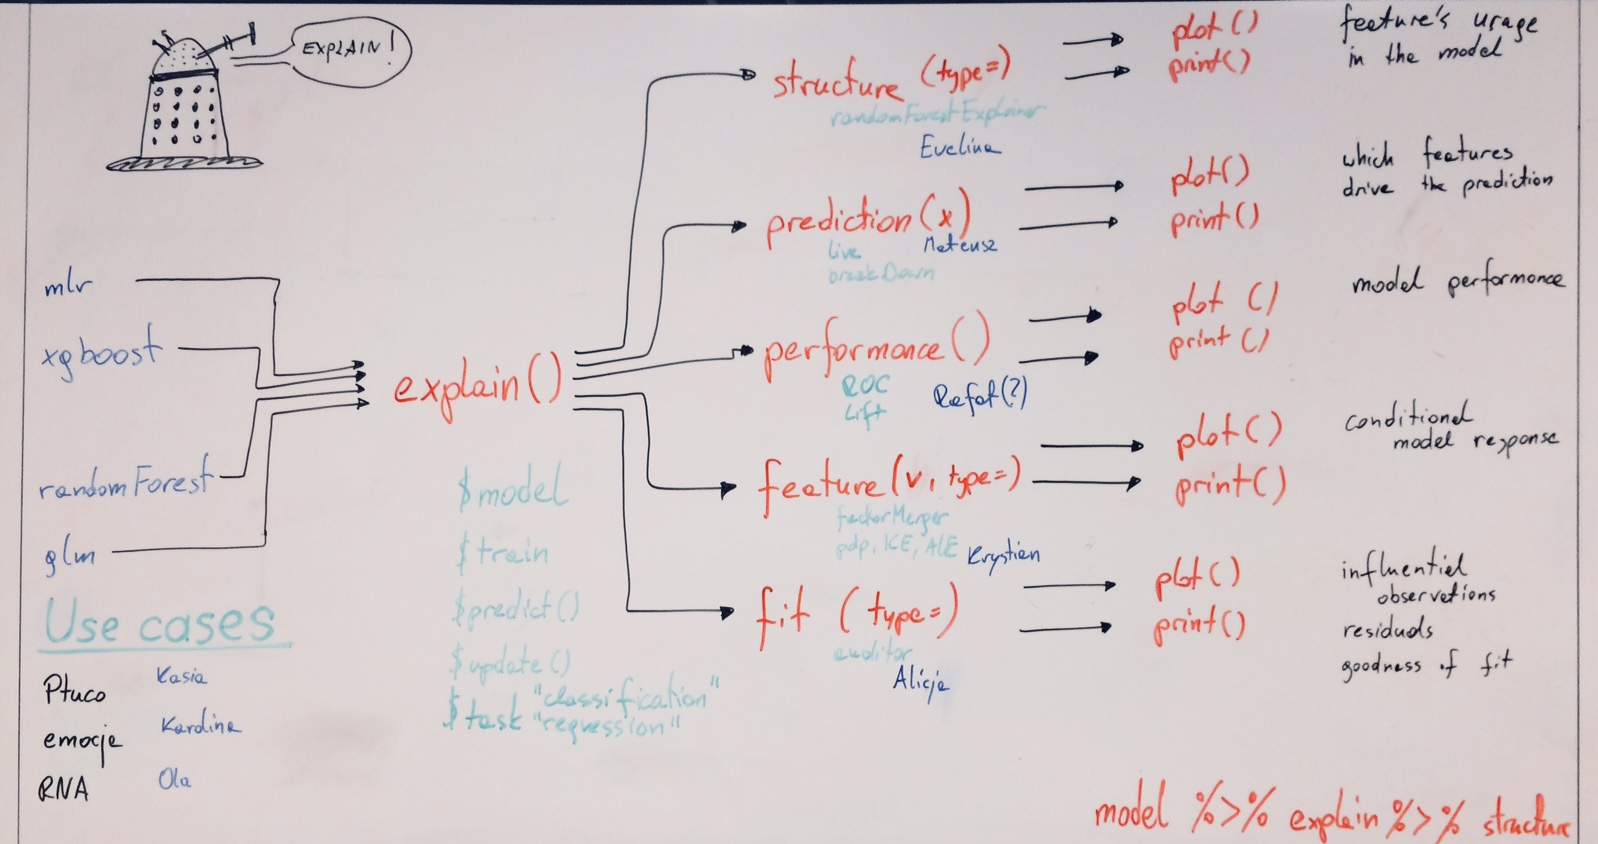
\includegraphics{images/DALEX_scheme.jpg}
\caption{Scheme}
\end{figure}

\citep{Strumbelj}, \citep{nnet_vis}, \citep{magix},
\citep{Zeiler_Fergus_2014}

\section{Notation}\label{notation}

This book describes explainers for different machine learning models.
Some of these explainers are created by different research groups with
different applications in mind.

To keep the notation consistent:

\begin{itemize}
\tightlist
\item
  \(x = (x_1, ..., x_p)\) stands for a vector of \(p\)
  variables/predictors.
\item
  \(y\) stands for a vector with target variable. In some applications
  it will be a continuous variable in others it will be a binary
  variable.
\item
  \(n\) stands for number of observations.
\item
  \(f(x, \theta)\) stands for a model. We are considering models that
  are characterized by a set of parameters \(\theta\). In some
  applications \(\theta\) is a low level space of parameters - nice
  parametric models, in some applications \(\theta\) may have a very
  complex structure.
\item
  \(\lambda\) stands for model meta-parameters which are not being
  directly optimized (like number of trees, max depth, some penalties
  etc.).
\item
  \(g(x)\) stands for a function that pre-process variables. In some
  applications it may be a standardisation or other pre-processing.
\end{itemize}

\begin{figure}
\centering
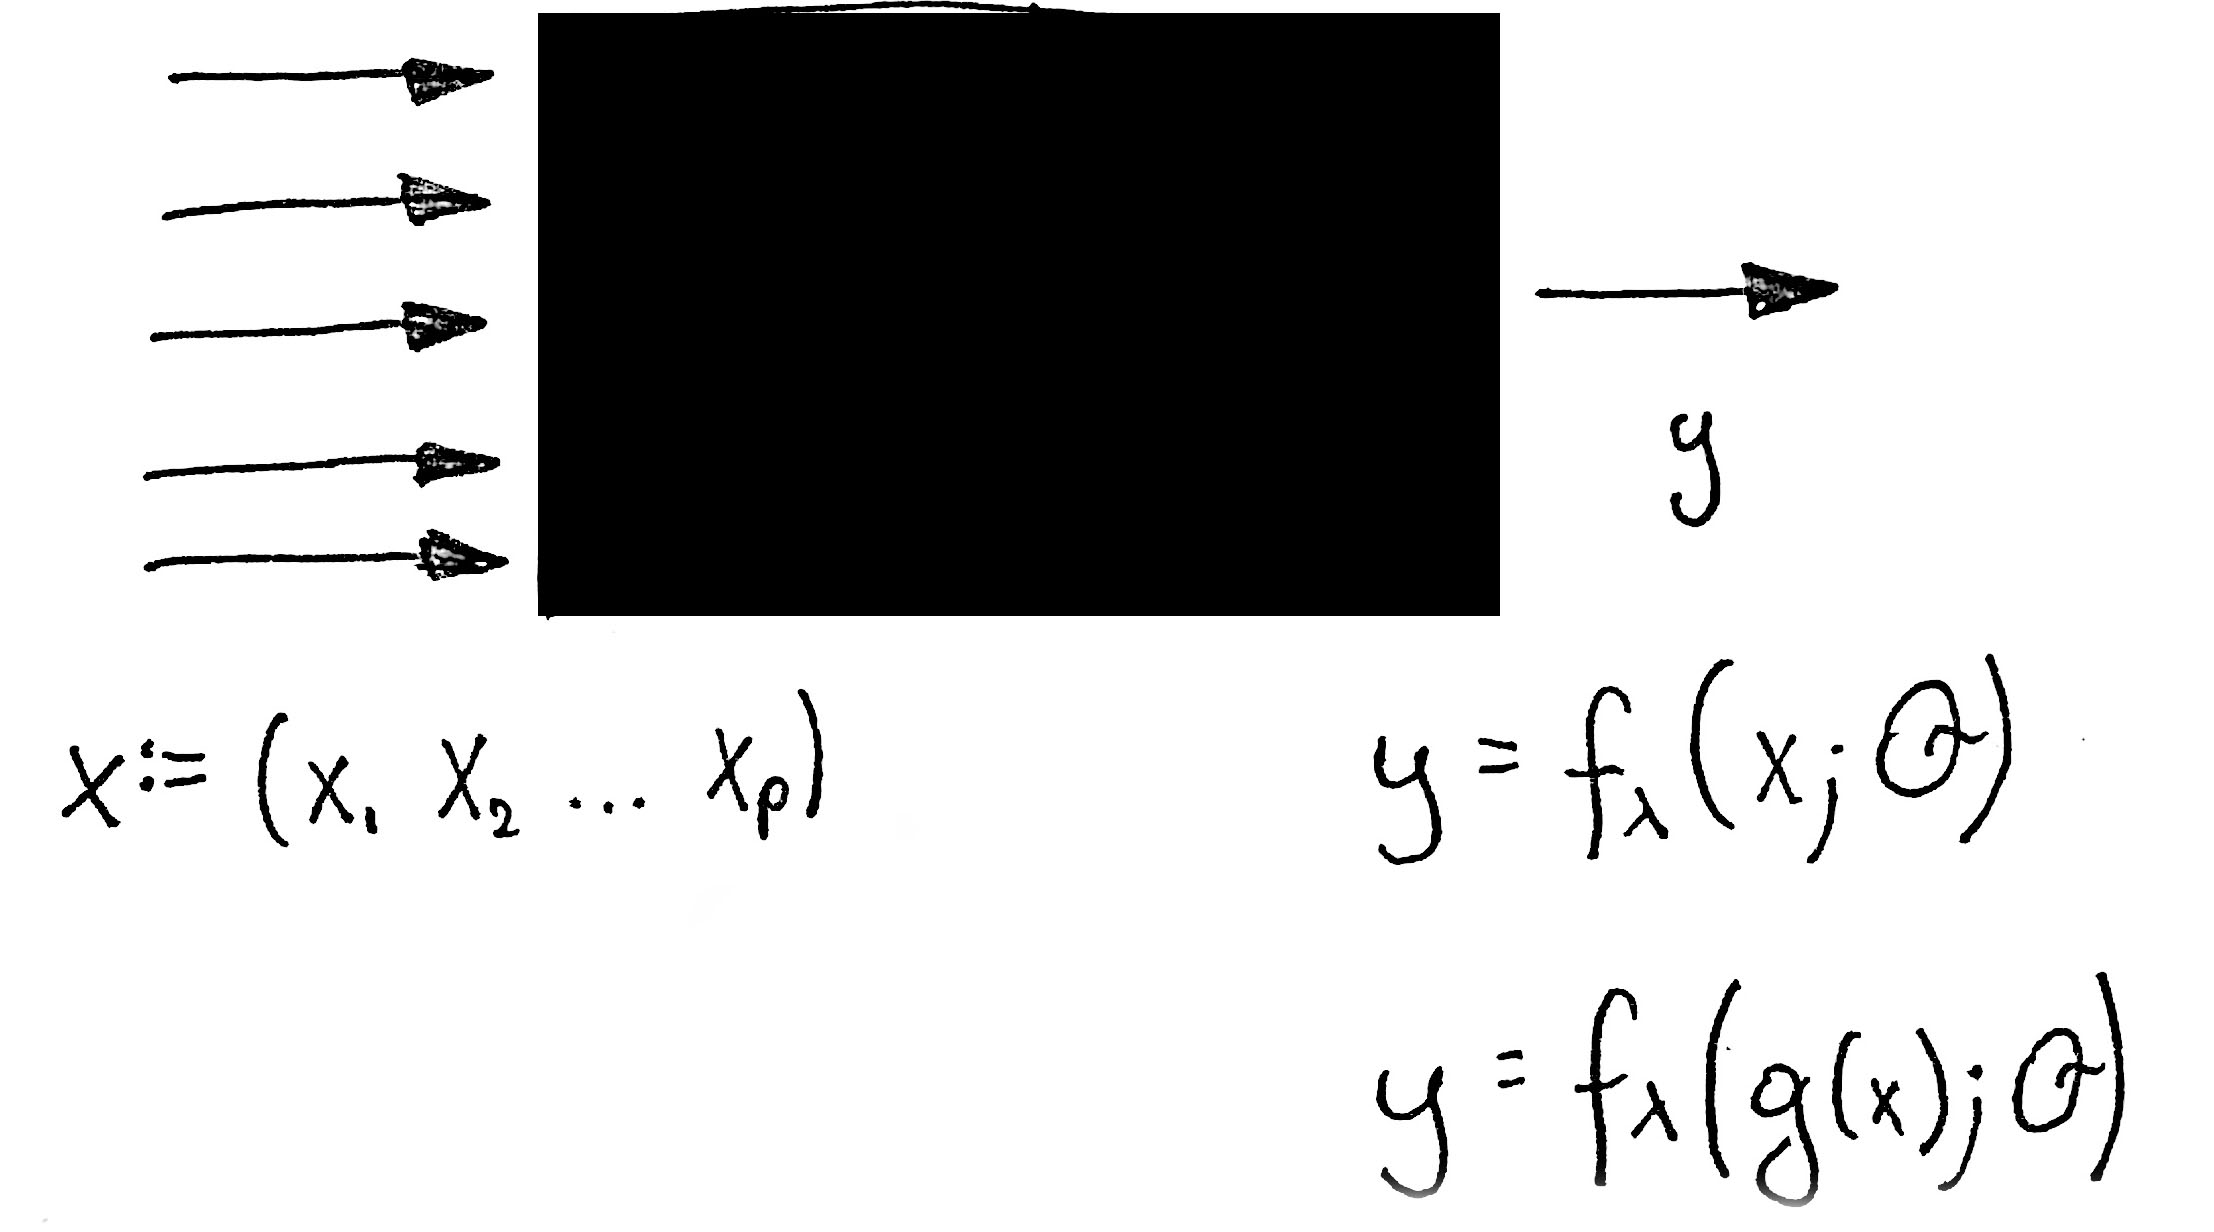
\includegraphics{images/model01.jpg}
\caption{}
\end{figure}

\section{Use case - Human Resources
Analytics}\label{use-case---human-resources-analytics}

To ilustrate applications of DALEX to binary classification problems we
will use a dataset from Kaggle competition
\href{https://www.kaggle.com/ludobenistant/hr-analytics/data}{Human
Resources Analytics}. This dataset is avaliable in the
\textbf{breakDown} package \citep{breakDown}.

\begin{Shaded}
\begin{Highlighting}[]
\KeywordTok{library}\NormalTok{(}\StringTok{"breakDown"}\NormalTok{)}
\KeywordTok{head}\NormalTok{(HR_data)}
\end{Highlighting}
\end{Shaded}

\begin{table}

\caption{(\#tab:hr_data)HR_data dataset from Kaggle competition Human Resources Analytics}
\centering
\begin{tabular}[t]{r|r|r|r|r|r|r|r|l|l}
\hline
satisfaction\_level & last\_evaluation & number\_project & average\_montly\_hours & time\_spend\_company & Work\_accident & left & promotion\_last\_5years & sales & salary\\
\hline
0.38 & 0.53 & 2 & 157 & 3 & 0 & 1 & 0 & sales & low\\
\hline
0.80 & 0.86 & 5 & 262 & 6 & 0 & 1 & 0 & sales & medium\\
\hline
0.11 & 0.88 & 7 & 272 & 4 & 0 & 1 & 0 & sales & medium\\
\hline
0.72 & 0.87 & 5 & 223 & 5 & 0 & 1 & 0 & sales & low\\
\hline
0.37 & 0.52 & 2 & 159 & 3 & 0 & 1 & 0 & sales & low\\
\hline
0.41 & 0.50 & 2 & 153 & 3 & 0 & 1 & 0 & sales & low\\
\hline
\end{tabular}
\end{table}

\subsection{Logistic regression}\label{logistic-regression}

In the following chapters to present explainers for logistic regression
models we will use \texttt{HR\_glm\_model}.

\begin{Shaded}
\begin{Highlighting}[]
\NormalTok{HR_glm_model <-}\StringTok{ }\KeywordTok{glm}\NormalTok{(left}\OperatorTok{~}\NormalTok{., }\DataTypeTok{data =}\NormalTok{ HR_data, }\DataTypeTok{family =} \StringTok{"binomial"}\NormalTok{)}
\KeywordTok{summary}\NormalTok{(HR_glm_model)}
\end{Highlighting}
\end{Shaded}

\begin{verbatim}
## 
## Call:
## glm(formula = left ~ ., family = "binomial", data = HR_data)
## 
## Deviance Residuals: 
##     Min       1Q   Median       3Q      Max  
## -2.2248  -0.6645  -0.4026  -0.1177   3.0688  
## 
## Coefficients:
##                         Estimate Std. Error z value Pr(>|z|)    
## (Intercept)           -1.4762862  0.1938373  -7.616 2.61e-14 ***
## satisfaction_level    -4.1356889  0.0980538 -42.178  < 2e-16 ***
## last_evaluation        0.7309032  0.1491787   4.900 9.61e-07 ***
## number_project        -0.3150787  0.0213248 -14.775  < 2e-16 ***
## average_montly_hours   0.0044603  0.0005161   8.643  < 2e-16 ***
## time_spend_company     0.2677537  0.0155736  17.193  < 2e-16 ***
## Work_accident         -1.5298283  0.0895473 -17.084  < 2e-16 ***
## promotion_last_5years -1.4301364  0.2574958  -5.554 2.79e-08 ***
## saleshr                0.2323779  0.1313084   1.770  0.07678 .  
## salesIT               -0.1807179  0.1221276  -1.480  0.13894    
## salesmanagement       -0.4484236  0.1598254  -2.806  0.00502 ** 
## salesmarketing        -0.0120882  0.1319304  -0.092  0.92700    
## salesproduct_mng      -0.1532529  0.1301538  -1.177  0.23901    
## salesRandD            -0.5823659  0.1448848  -4.020 5.83e-05 ***
## salessales            -0.0387859  0.1024006  -0.379  0.70486    
## salessupport           0.0500251  0.1092834   0.458  0.64713    
## salestechnical         0.0701464  0.1065379   0.658  0.51027    
## salarylow              1.9440627  0.1286272  15.114  < 2e-16 ***
## salarymedium           1.4132244  0.1293534  10.925  < 2e-16 ***
## ---
## Signif. codes:  0 '***' 0.001 '**' 0.01 '*' 0.05 '.' 0.1 ' ' 1
## 
## (Dispersion parameter for binomial family taken to be 1)
## 
##     Null deviance: 16465  on 14998  degrees of freedom
## Residual deviance: 12850  on 14980  degrees of freedom
## AIC: 12888
## 
## Number of Fisher Scoring iterations: 5
\end{verbatim}

Models used in this doccumentation are accessible via \textbf{archivist}
package. To download the \texttt{HR\_glm\_model} model use the following
instruction.

\begin{verbatim}
archivist::aread("pbiecek/DALEX/arepo/8fe19a108faf3ddfcabc3de3a0693234")
\end{verbatim}

\subsection{Random forest}\label{random-forest}

In the following chapters to present explainers for random forest models
we will use \texttt{HR\_fr\_model}.

\begin{Shaded}
\begin{Highlighting}[]
\KeywordTok{library}\NormalTok{(}\StringTok{"randomForest"}\NormalTok{)}
\KeywordTok{set.seed}\NormalTok{(}\DecValTok{1313}\NormalTok{)}
\NormalTok{HR_data}\OperatorTok{$}\NormalTok{left <-}\StringTok{ }\KeywordTok{factor}\NormalTok{(HR_data}\OperatorTok{$}\NormalTok{left)}
\NormalTok{HR_rf_model <-}\StringTok{ }\KeywordTok{randomForest}\NormalTok{(left}\OperatorTok{~}\NormalTok{., }\DataTypeTok{data =}\NormalTok{ HR_data, }\DataTypeTok{ntree =} \DecValTok{100}\NormalTok{)}
\NormalTok{HR_rf_model}
\end{Highlighting}
\end{Shaded}

\begin{verbatim}
## 
## Call:
##  randomForest(formula = left ~ ., data = HR_data, ntree = 100) 
##                Type of random forest: classification
##                      Number of trees: 100
## No. of variables tried at each split: 3
## 
##         OOB estimate of  error rate: 0.75%
## Confusion matrix:
##       0    1 class.error
## 0 11407   21 0.001837592
## 1    91 3480 0.025483058
\end{verbatim}

Models used in this doccumentation are accessible via \textbf{archivist}
package. To download the \texttt{HR\_rf\_model} model use the following
instruction.

\begin{verbatim}
archivist::aread("pbiecek/DALEX/arepo/419d550a92fab6a5f28650130991e2cd")
\end{verbatim}

\section{Use case - Wine quality}\label{use-case---wine-quality}

To ilustrate applications of DALEX to regression problems we will use a
Wine quality dataset from Kaggle competition
\href{http://mlr.cs.umass.edu/ml/}{UC Irvine Machine Learning
Repository}.

\begin{Shaded}
\begin{Highlighting}[]
\NormalTok{url <-}\StringTok{ 'https://archive.ics.uci.edu/ml/machine-learning-databases/wine-quality/winequality-white.csv'}
\NormalTok{wine <-}\StringTok{ }\KeywordTok{read.table}\NormalTok{(url, }\DataTypeTok{header =} \OtherTok{TRUE}\NormalTok{, }\DataTypeTok{sep =} \StringTok{";"}\NormalTok{)}
\KeywordTok{head}\NormalTok{(wine)}
\end{Highlighting}
\end{Shaded}

\begin{table}

\caption{\label{tab:wineQuality}Wine quality dataset from UC Irvine Machine Learning Repository}
\centering
\begin{tabular}[t]{r|r|r|r|r|r|r|r|r|r|r|r}
\hline
fixed.acidity & volatile.acidity & citric.acid & residual.sugar & chlorides & free.sulfur.dioxide & total.sulfur.dioxide & density & pH & sulphates & alcohol & quality\\
\hline
7.0 & 0.27 & 0.36 & 20.7 & 0.045 & 45 & 170 & 1.0010 & 3.00 & 0.45 & 8.8 & 6\\
\hline
6.3 & 0.30 & 0.34 & 1.6 & 0.049 & 14 & 132 & 0.9940 & 3.30 & 0.49 & 9.5 & 6\\
\hline
8.1 & 0.28 & 0.40 & 6.9 & 0.050 & 30 & 97 & 0.9951 & 3.26 & 0.44 & 10.1 & 6\\
\hline
7.2 & 0.23 & 0.32 & 8.5 & 0.058 & 47 & 186 & 0.9956 & 3.19 & 0.40 & 9.9 & 6\\
\hline
7.2 & 0.23 & 0.32 & 8.5 & 0.058 & 47 & 186 & 0.9956 & 3.19 & 0.40 & 9.9 & 6\\
\hline
8.1 & 0.28 & 0.40 & 6.9 & 0.050 & 30 & 97 & 0.9951 & 3.26 & 0.44 & 10.1 & 6\\
\hline
\end{tabular}
\end{table}

\subsection{Linear regression}\label{linear-regression}

In the following chapters to present explainers for gaussian regression
models we will use \texttt{wine\_lm\_model}.

\begin{Shaded}
\begin{Highlighting}[]
\NormalTok{wine_lm_model <-}\StringTok{ }\KeywordTok{lm}\NormalTok{(quality }\OperatorTok{~}\StringTok{ }\NormalTok{fixed.acidity }\OperatorTok{+}\StringTok{ }\NormalTok{volatile.acidity }\OperatorTok{+}\StringTok{ }\NormalTok{citric.acid }\OperatorTok{+}\StringTok{ }\NormalTok{residual.sugar }\OperatorTok{+}\StringTok{ }\NormalTok{chlorides }\OperatorTok{+}\StringTok{ }\NormalTok{free.sulfur.dioxide }\OperatorTok{+}\StringTok{ }\NormalTok{total.sulfur.dioxide }\OperatorTok{+}\StringTok{ }\NormalTok{density }\OperatorTok{+}\StringTok{ }\NormalTok{pH }\OperatorTok{+}\StringTok{ }\NormalTok{sulphates }\OperatorTok{+}\StringTok{ }\NormalTok{alcohol,}
               \DataTypeTok{data =}\NormalTok{ wine)}
\end{Highlighting}
\end{Shaded}

Models used in this doccumentation are accessible via \textbf{archivist}
package. To download the \texttt{wine\_lm\_model} model use the
following instruction.

\begin{verbatim}
archivist::aread("pbiecek/DALEX/arepo/b99a3d58016e2677221019652cff047f")
\end{verbatim}

\section{Trivia}\label{trivia}

\begin{figure}
\centering

\includegraphics{images/dalex01small.jpg}
\caption{}
\end{figure}

\href{https://en.wikipedia.org/wiki/Dalek}{The Daleks} are a fictional
extraterrestrial race portrayed in the
\href{https://en.wikipedia.org/wiki/Doctor_Who}{Doctor Who} BBC series.
Rather dim aliens, known to repeat the phrase \emph{Explain!} very
often.

\chapter{Global structure}\label{global-structure}

Explainers presented in this chapter are designed to better understand
the global structure of a black box. Which variables are the most
important? How do they influence the final result of a model?

\section{Drop-out plots}\label{drop-out-plots}

Variable drop-outs are calculated via permutations. Simply the loss
function is is compared between the full model and the model with single
variable being permuted.

As a additional point for comparison a \texttt{\_baseline\_} is
calculated as a loss in model with permuted outcomes. This shall be
highest possible loss.

Let's see how it's working for a random forest model.

\begin{Shaded}
\begin{Highlighting}[]
\KeywordTok{library}\NormalTok{(}\StringTok{"DALEX"}\NormalTok{)}
\KeywordTok{library}\NormalTok{(}\StringTok{"randomForest"}\NormalTok{)}
\NormalTok{HR_rf_model <-}\StringTok{ }\KeywordTok{randomForest}\NormalTok{(left}\OperatorTok{~}\NormalTok{., }\DataTypeTok{data =}\NormalTok{ breakDown}\OperatorTok{::}\NormalTok{HR_data, }\DataTypeTok{ntree =} \DecValTok{100}\NormalTok{)}
\NormalTok{explainer_rf  <-}\StringTok{ }\KeywordTok{explain}\NormalTok{(HR_rf_model, }\DataTypeTok{data =}\NormalTok{ HR_data, }\DataTypeTok{y =}\NormalTok{ HR_data}\OperatorTok{$}\NormalTok{left)}
\NormalTok{vd_rf <-}\StringTok{ }\KeywordTok{variable_dropout}\NormalTok{(explainer_rf, }\DataTypeTok{type =} \StringTok{"raw"}\NormalTok{)}
\NormalTok{vd_rf}
\end{Highlighting}
\end{Shaded}

\begin{verbatim}
##       variable dropout_loss        label
## 1 _full_model_           NA randomForest
## 2   _baseline_           NA randomForest
\end{verbatim}

Now we can plot these losses. Note that in the plot beow you see not
only the variable importance, but also you see how the whole model
works.

\begin{Shaded}
\begin{Highlighting}[]
\KeywordTok{plot}\NormalTok{(vd_rf)}
\end{Highlighting}
\end{Shaded}

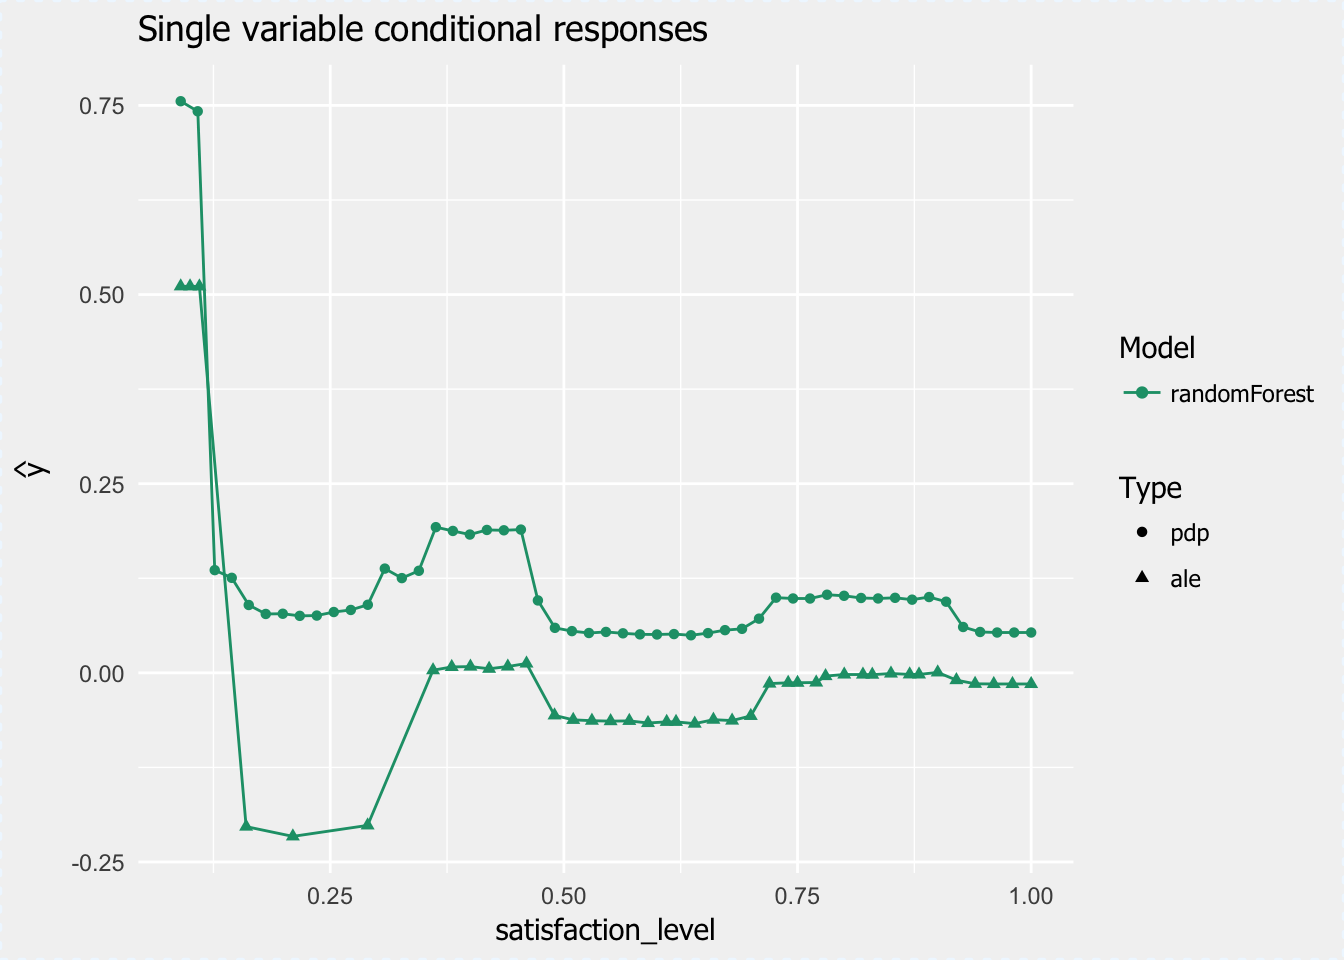
\includegraphics{DALEX_files/figure-latex/unnamed-chunk-10-1.pdf}

And here we have similar example for glm model.

\begin{Shaded}
\begin{Highlighting}[]
\NormalTok{HR_glm_model <-}\StringTok{ }\KeywordTok{glm}\NormalTok{(left}\OperatorTok{~}\NormalTok{., }\DataTypeTok{data =}\NormalTok{ breakDown}\OperatorTok{::}\NormalTok{HR_data, }\DataTypeTok{family =} \StringTok{"binomial"}\NormalTok{)}
\NormalTok{explainer_glm <-}\StringTok{ }\KeywordTok{explain}\NormalTok{(HR_glm_model, }\DataTypeTok{data =}\NormalTok{ HR_data, }\DataTypeTok{y =}\NormalTok{ HR_data}\OperatorTok{$}\NormalTok{left)}
\NormalTok{logit <-}\StringTok{ }\ControlFlowTok{function}\NormalTok{(x) }\KeywordTok{exp}\NormalTok{(x)}\OperatorTok{/}\NormalTok{(}\DecValTok{1}\OperatorTok{+}\KeywordTok{exp}\NormalTok{(x))}
\NormalTok{vd_glm <-}\StringTok{ }\KeywordTok{variable_dropout}\NormalTok{(explainer_glm, }\DataTypeTok{type =} \StringTok{"raw"}\NormalTok{,}
                        \DataTypeTok{loss_function =} \ControlFlowTok{function}\NormalTok{(observed, predicted) }\KeywordTok{sum}\NormalTok{((observed }\OperatorTok{-}\StringTok{ }\KeywordTok{logit}\NormalTok{(predicted))}\OperatorTok{^}\DecValTok{2}\NormalTok{))}
\NormalTok{vd_glm}
\end{Highlighting}
\end{Shaded}

\begin{verbatim}
##       variable dropout_loss label
## 1 _full_model_           NA    lm
## 2   _baseline_           NA    lm
\end{verbatim}

\begin{Shaded}
\begin{Highlighting}[]
\KeywordTok{plot}\NormalTok{(vd_glm)}
\end{Highlighting}
\end{Shaded}

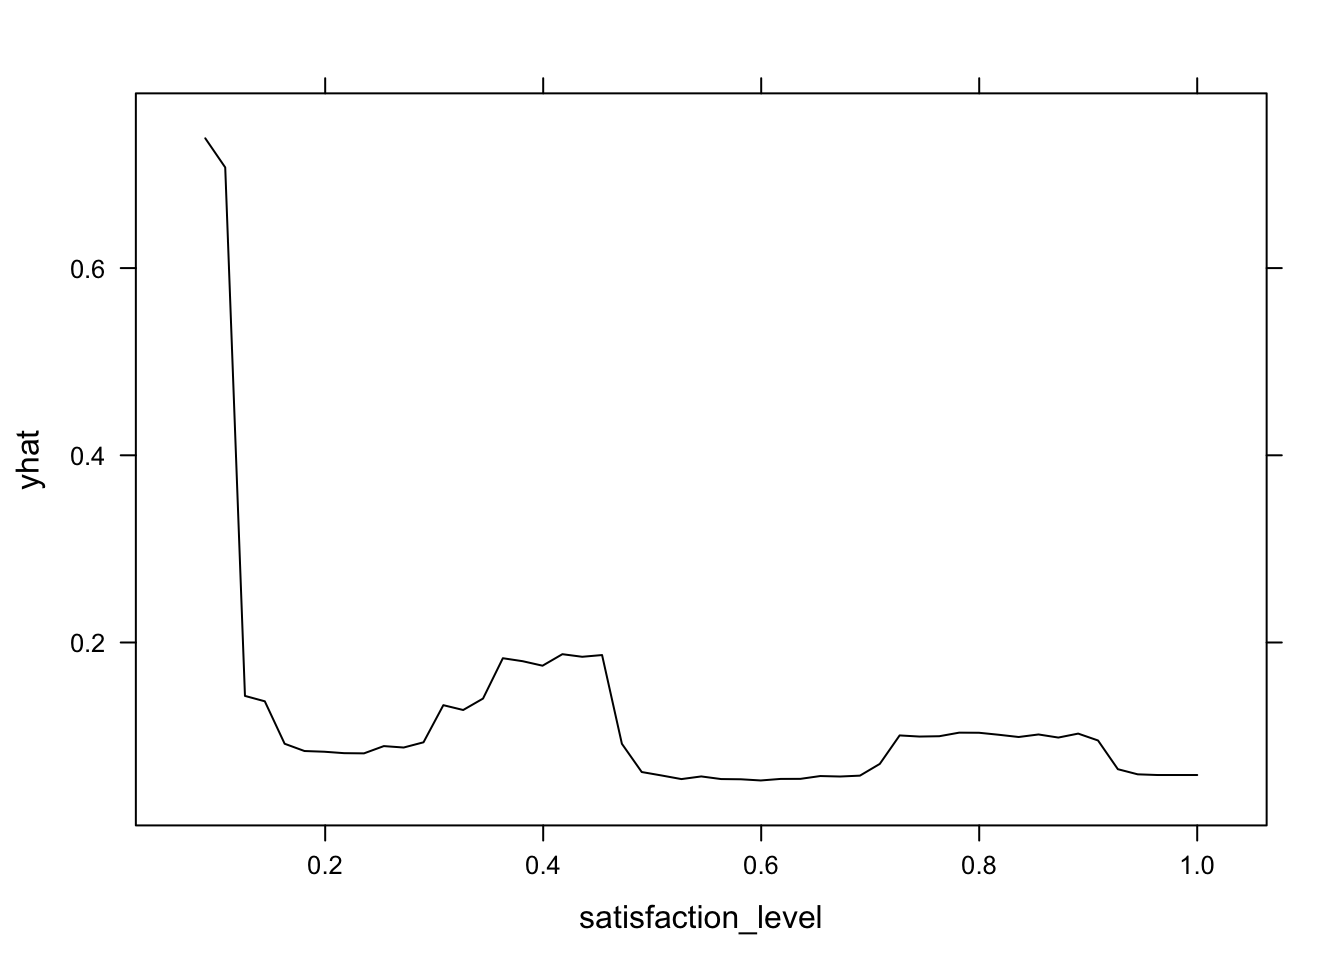
\includegraphics{DALEX_files/figure-latex/unnamed-chunk-11-1.pdf}

And for xgboost model.

\begin{Shaded}
\begin{Highlighting}[]
\KeywordTok{library}\NormalTok{(}\StringTok{"xgboost"}\NormalTok{)}
\NormalTok{model_martix_train <-}\StringTok{ }\KeywordTok{model.matrix}\NormalTok{(left}\OperatorTok{~}\NormalTok{.}\OperatorTok{-}\DecValTok{1}\NormalTok{, breakDown}\OperatorTok{::}\NormalTok{HR_data)}
\NormalTok{data_train <-}\StringTok{ }\KeywordTok{xgb.DMatrix}\NormalTok{(model_martix_train, }\DataTypeTok{label =}\NormalTok{ breakDown}\OperatorTok{::}\NormalTok{HR_data}\OperatorTok{$}\NormalTok{left)}
\NormalTok{param <-}\StringTok{ }\KeywordTok{list}\NormalTok{(}\DataTypeTok{max_depth =} \DecValTok{2}\NormalTok{, }\DataTypeTok{eta =} \DecValTok{1}\NormalTok{, }\DataTypeTok{silent =} \DecValTok{1}\NormalTok{, }\DataTypeTok{nthread =} \DecValTok{2}\NormalTok{,}
              \DataTypeTok{objective =} \StringTok{"binary:logistic"}\NormalTok{, }\DataTypeTok{eval_metric =} \StringTok{"auc"}\NormalTok{)}
\NormalTok{HR_xgb_model <-}\StringTok{ }\KeywordTok{xgb.train}\NormalTok{(param, data_train, }\DataTypeTok{nrounds =} \DecValTok{50}\NormalTok{)}
\NormalTok{explainer_xgb <-}\StringTok{ }\KeywordTok{explain}\NormalTok{(HR_xgb_model, }\DataTypeTok{data =}\NormalTok{ model_martix_train, }\DataTypeTok{y =}\NormalTok{ HR_data}\OperatorTok{$}\NormalTok{left, }\DataTypeTok{label =} \StringTok{"xgboost"}\NormalTok{)}
\NormalTok{vd_xgb <-}\StringTok{ }\KeywordTok{variable_dropout}\NormalTok{(explainer_xgb, }\DataTypeTok{type =} \StringTok{"raw"}\NormalTok{)}
\NormalTok{vd_xgb}
\end{Highlighting}
\end{Shaded}

\begin{verbatim}
##       variable dropout_loss   label
## 1 _full_model_           NA xgboost
## 2   _baseline_           NA xgboost
\end{verbatim}

\begin{Shaded}
\begin{Highlighting}[]
\KeywordTok{plot}\NormalTok{(vd_xgb)}
\end{Highlighting}
\end{Shaded}

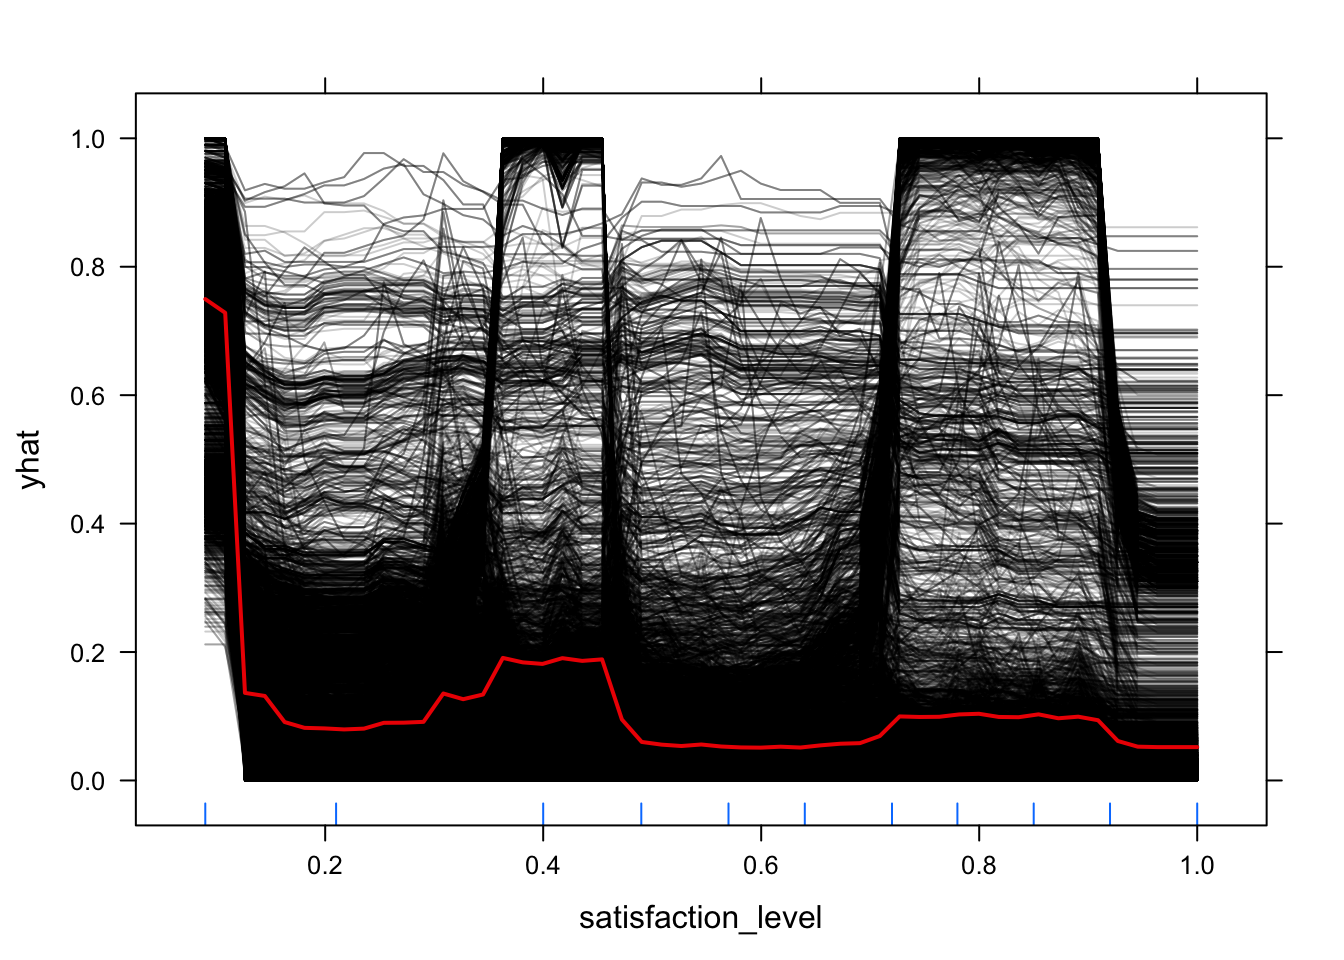
\includegraphics{DALEX_files/figure-latex/unnamed-chunk-12-1.pdf}

Of course you can plot all these models in a single plot. Then it is
much easier to compare variable importances in different models.

\begin{Shaded}
\begin{Highlighting}[]
\KeywordTok{plot}\NormalTok{(vd_rf, vd_glm, vd_xgb)}
\end{Highlighting}
\end{Shaded}

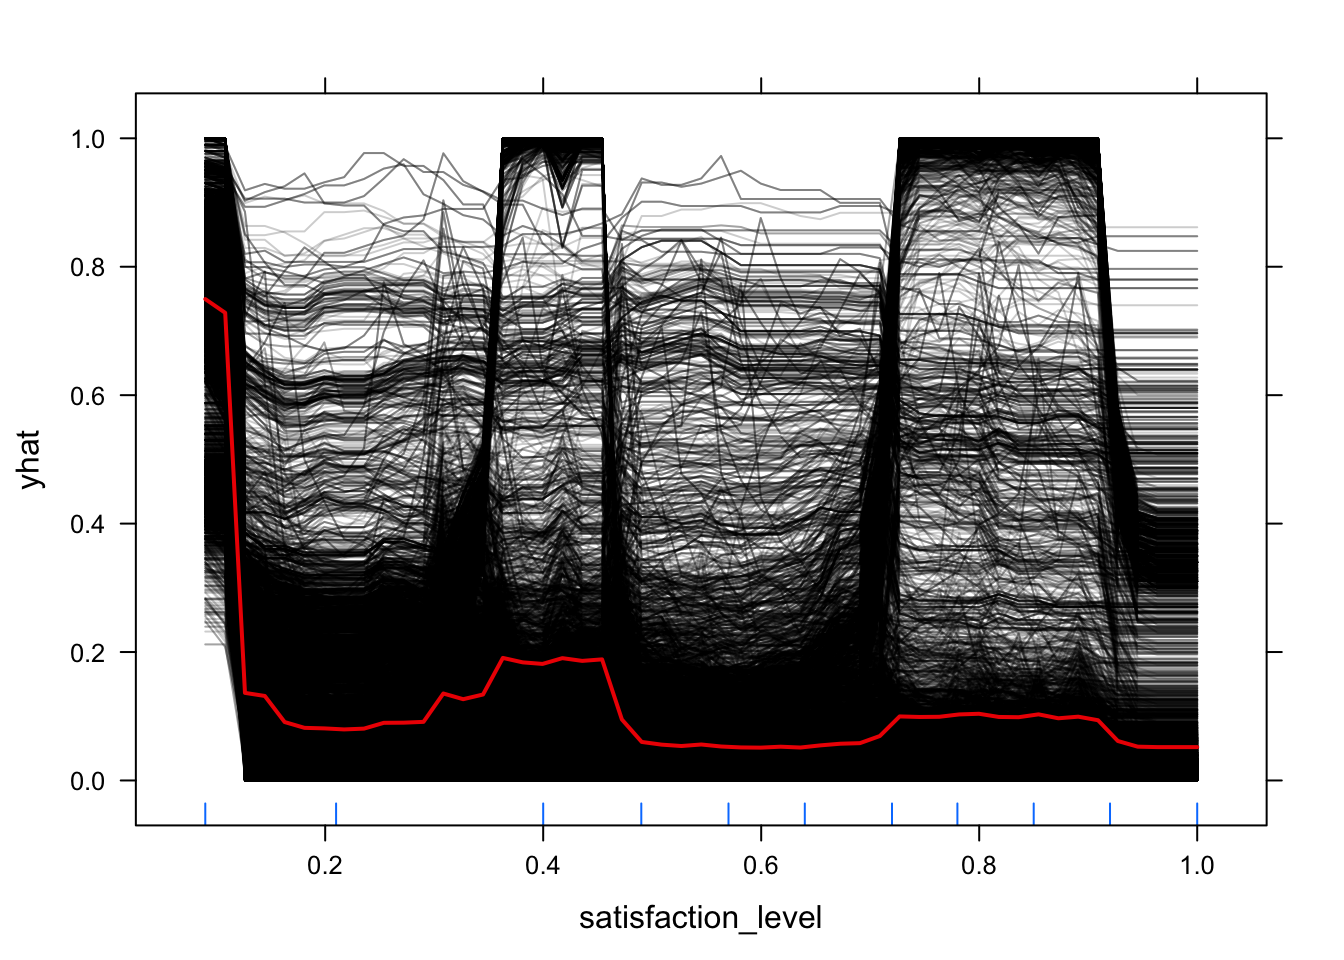
\includegraphics{DALEX_files/figure-latex/unnamed-chunk-13-1.pdf}

\emph{NOTE:} If you like to have all importances hooked to 0, you can do
this as well

\begin{Shaded}
\begin{Highlighting}[]
\NormalTok{vd_rf <-}\StringTok{ }\KeywordTok{variable_dropout}\NormalTok{(explainer_rf, }\DataTypeTok{type =} \StringTok{"difference"}\NormalTok{)}
\NormalTok{vd_glm <-}\StringTok{ }\KeywordTok{variable_dropout}\NormalTok{(explainer_glm, }\DataTypeTok{type =} \StringTok{"difference"}\NormalTok{,}
                        \DataTypeTok{loss_function =} \ControlFlowTok{function}\NormalTok{(observed, predicted) }\KeywordTok{sum}\NormalTok{((observed }\OperatorTok{-}\StringTok{ }\KeywordTok{logit}\NormalTok{(predicted))}\OperatorTok{^}\DecValTok{2}\NormalTok{))}
\NormalTok{vd_xgb <-}\StringTok{ }\KeywordTok{variable_dropout}\NormalTok{(explainer_xgb, }\DataTypeTok{type =} \StringTok{"difference"}\NormalTok{)}
\KeywordTok{plot}\NormalTok{(vd_rf, vd_glm, vd_xgb)}
\end{Highlighting}
\end{Shaded}

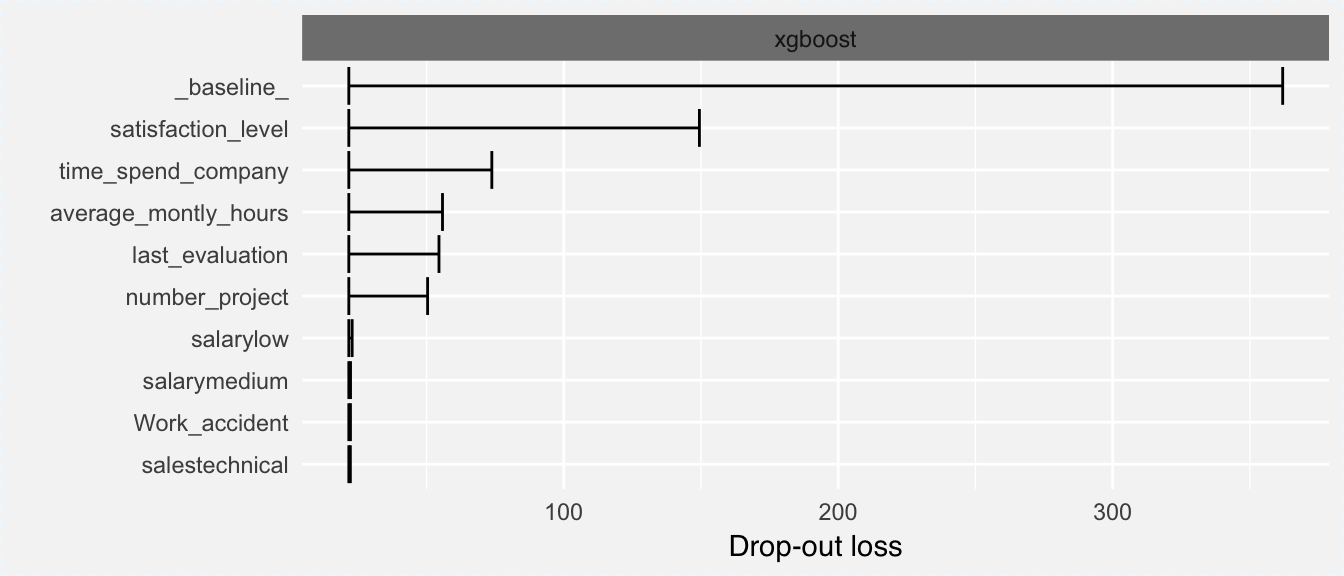
\includegraphics{DALEX_files/figure-latex/unnamed-chunk-14-1.pdf}

\section{Forest plots}\label{forest-plots}

\href{https://en.wikipedia.org/wiki/Forest_plot}{Forest plots} were
initially used in the meta analysis to visualise effects in different
studies. But now they are frequently used to present summary
characteristics for models with linear structure like these created with
\texttt{lm} or \texttt{glm} functions.

There are various implementations of forest plots in R. Below we present
examples for a glm model.

\begin{Shaded}
\begin{Highlighting}[]
\KeywordTok{library}\NormalTok{(}\StringTok{"breakDown"}\NormalTok{)}
\NormalTok{HR_glm_model <-}\StringTok{ }\KeywordTok{glm}\NormalTok{(left}\OperatorTok{~}\NormalTok{., }\DataTypeTok{data =}\NormalTok{ HR_data, }\DataTypeTok{family =} \StringTok{"binomial"}\NormalTok{)}


\CommentTok{#HR_glm_model <- archivist::aread("pbiecek/DALEX/arepo/8fe19a108faf3ddfcabc3de3a0693234")}
\end{Highlighting}
\end{Shaded}

In the package \textbf{forestmodel} (see \citep{forestmodel}) one can
use \texttt{forest\_model()} function to draw a forest plot. This
package is based on the \textbf{broom} package (see \citep{broom}) and
this is why it handles a large variety of different regression models.
An example for \texttt{glm}.

\begin{Shaded}
\begin{Highlighting}[]
\KeywordTok{library}\NormalTok{(}\StringTok{"forestmodel"}\NormalTok{)}
\KeywordTok{forest_model}\NormalTok{(HR_glm_model)}
\end{Highlighting}
\end{Shaded}

\begin{figure}
\centering
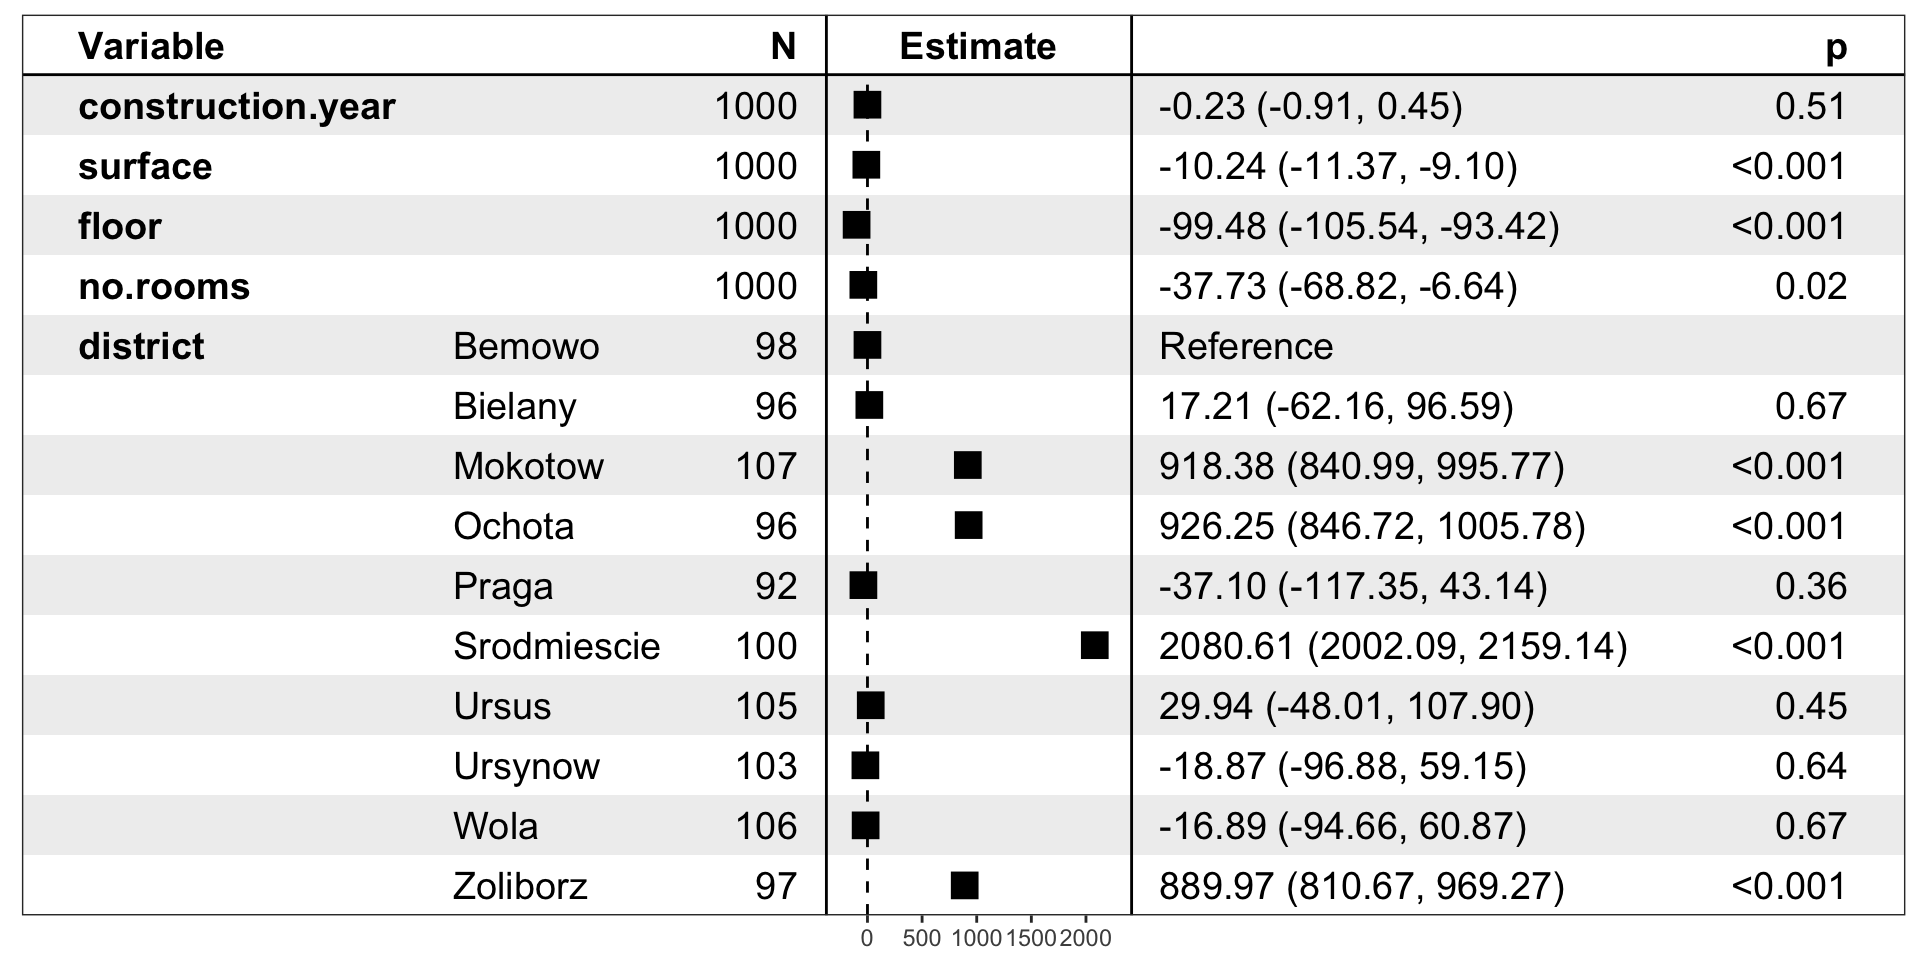
\includegraphics{DALEX_files/figure-latex/forestmodel-1.pdf}
\caption{\label{fig:forestmodel}Forest plot created with forestmodel
package}
\end{figure}

In the package \textbf{sjPlot} (see \citep{sjPlot}) one can use
\texttt{sjp.*()} to visualise structure of a \texttt{*} model or a
wrapper \texttt{plot\_model()}. Here is an example for \texttt{glm}
model.

\begin{Shaded}
\begin{Highlighting}[]
\KeywordTok{library}\NormalTok{(}\StringTok{"sjPlot"}\NormalTok{)}
\KeywordTok{plot_model}\NormalTok{(HR_glm_model, }\DataTypeTok{type =} \StringTok{"est"}\NormalTok{, }\DataTypeTok{sort.est =} \OtherTok{TRUE}\NormalTok{)}
\end{Highlighting}
\end{Shaded}

\begin{figure}
\centering
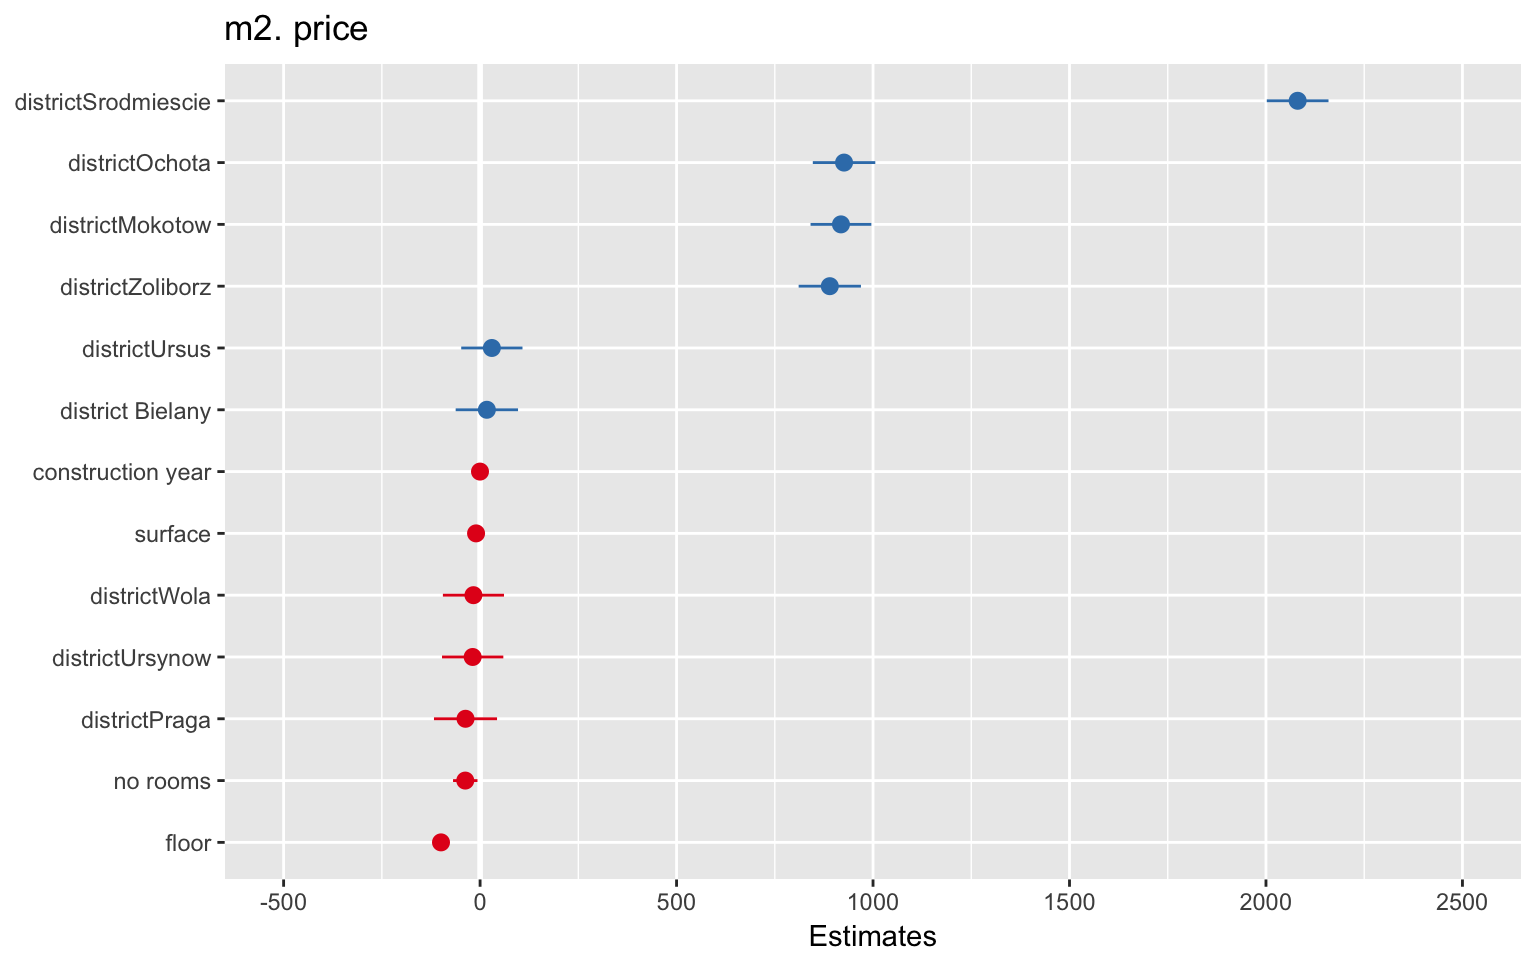
\includegraphics{DALEX_files/figure-latex/sjpglm-1.pdf}
\caption{\label{fig:sjpglm}Forest plot created with sjPlot package}
\end{figure}

\textbf{Note!}

The \textbf{forestmodel} package handles factor variables in a better
way while the plots from \textbf{sjPlot} are easier to read.

\section{Variable Importance Plot}\label{variable-importance-plot}

\section{ctree}\label{ctree}

\section{RandomForestExplainer}\label{randomforestexplainer}

\chapter{Conditional structure}\label{conditional-structure}

\begin{figure}
\centering
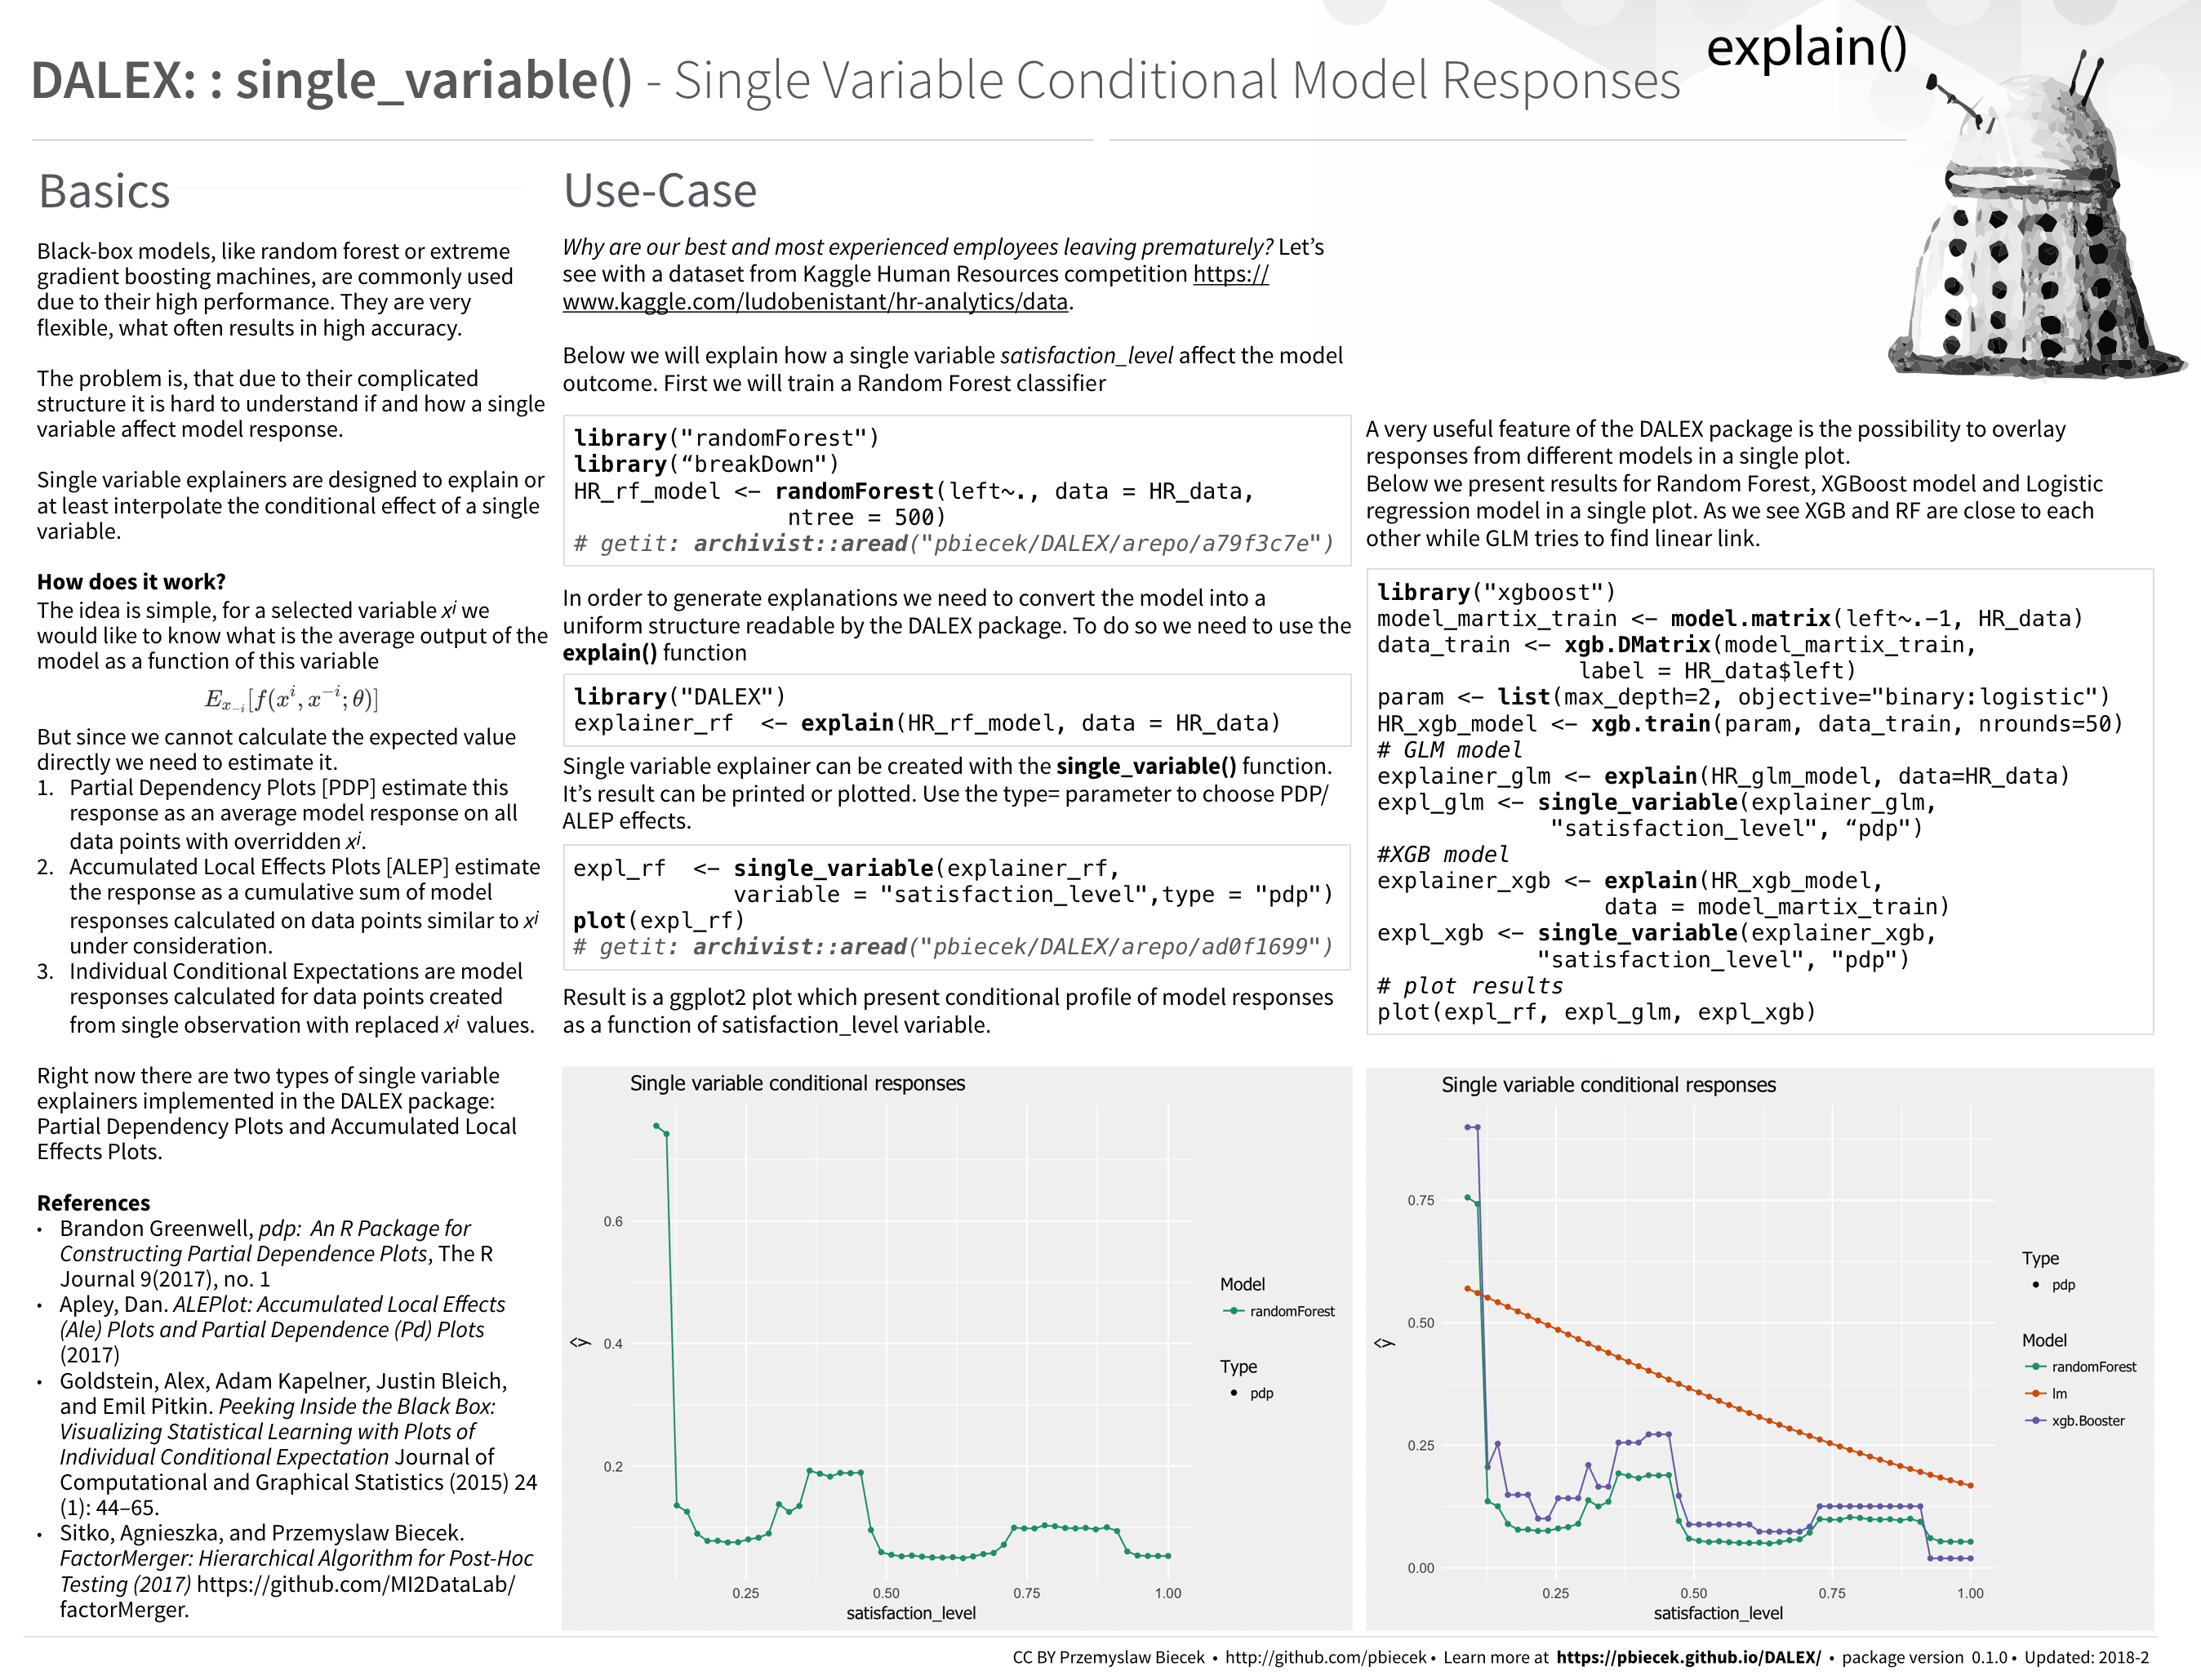
\includegraphics{images/DALEX_single_variable.png}
\caption{Cheatsheet}
\end{figure}

The dimension of input \(x\) for black box models is usually high (large
\(p\)). But in many cases small number of variables play important role
in the model OR there are some reasons to believe that variables work in
an additive fashion/low-level interactions in the model.

In such cases one may be interesting in verification how the conditional
response for a selected interesting variable/variables looks like.

Methods presented below help to understand the conditional structure of
a model.

\section{Partial Dependence Plot}\label{pdpchapter}

Partial Dependence Plots (see \textbf{pdp} package \citep{pdp}) for a
black box \(f(x; \theta)\) calculates the expected output given a
selected variable.

\[
p_i(x_i) = E_{x_{-i}}[ f(x^i, x^{-i}; \theta) ]
\]

Of course this expectation cannot be calculated directly as we do not
know fully the \(f()\) neither the distribution of \(x_{-i}\). This
value is estimated by

\[
\hat p_i(x_i) = \frac{1}{n} \sum_{j=1}^{n} f(x^i_j, x_j^{-i}, \hat \theta) 
\]

Let's see an example for the model \texttt{HR\_rf\_model}. Below we are
using \texttt{DALEX::single\_variable} function that is calling
\texttt{pdp::partial} function to calculate pdp curve for variable
\texttt{satisfaction\_level}. Then the curve is plotted with generic
\texttt{plot.single\_variable\_explainer()} function.

Marginal response plots are created in four steps.

\begin{enumerate}
\def\labelenumi{\arabic{enumi}.}
\tightlist
\item
  We need to fit model. For example a Random Forest model.
\end{enumerate}

\begin{Shaded}
\begin{Highlighting}[]
\KeywordTok{library}\NormalTok{(}\StringTok{"randomForest"}\NormalTok{)}
\KeywordTok{library}\NormalTok{(}\StringTok{"breakDown"}\NormalTok{)}

\NormalTok{HR_rf_model <-}\StringTok{ }\KeywordTok{randomForest}\NormalTok{(left}\OperatorTok{~}\NormalTok{., }\DataTypeTok{data =}\NormalTok{ breakDown}\OperatorTok{::}\NormalTok{HR_data, }\DataTypeTok{ntree =} \DecValTok{100}\NormalTok{)}
\CommentTok{# a79f3c7ec27499fb91e46ee70d423ac8}
\CommentTok{# archivist::aread("pbiecek/DALEX/arepo/a79f3c7ec27")}
\end{Highlighting}
\end{Shaded}

\begin{enumerate}
\def\labelenumi{\arabic{enumi}.}
\setcounter{enumi}{1}
\tightlist
\item
  We need to create an explainer. It's an interface that can be used to
  explain a black-box model.
\end{enumerate}

\begin{Shaded}
\begin{Highlighting}[]
\KeywordTok{library}\NormalTok{(}\StringTok{"DALEX"}\NormalTok{)}
\NormalTok{explainer_rf  <-}\StringTok{ }\KeywordTok{explain}\NormalTok{(HR_rf_model, }\DataTypeTok{data =}\NormalTok{ HR_data)}
\end{Highlighting}
\end{Shaded}

\begin{enumerate}
\def\labelenumi{\arabic{enumi}.}
\setcounter{enumi}{2}
\tightlist
\item
  Now we can calculate the marginal response with the PDP method.
\end{enumerate}

\begin{Shaded}
\begin{Highlighting}[]
\NormalTok{expl_rf  <-}\StringTok{ }\KeywordTok{single_variable}\NormalTok{(explainer_rf, }\DataTypeTok{variable =}  \StringTok{"satisfaction_level"}\NormalTok{, }\DataTypeTok{type =} \StringTok{"pdp"}\NormalTok{)}
\end{Highlighting}
\end{Shaded}

\begin{enumerate}
\def\labelenumi{\arabic{enumi}.}
\setcounter{enumi}{3}
\tightlist
\item
  And we are ready to plot it.
\end{enumerate}

\begin{Shaded}
\begin{Highlighting}[]
\KeywordTok{plot}\NormalTok{(expl_rf)}
\end{Highlighting}
\end{Shaded}

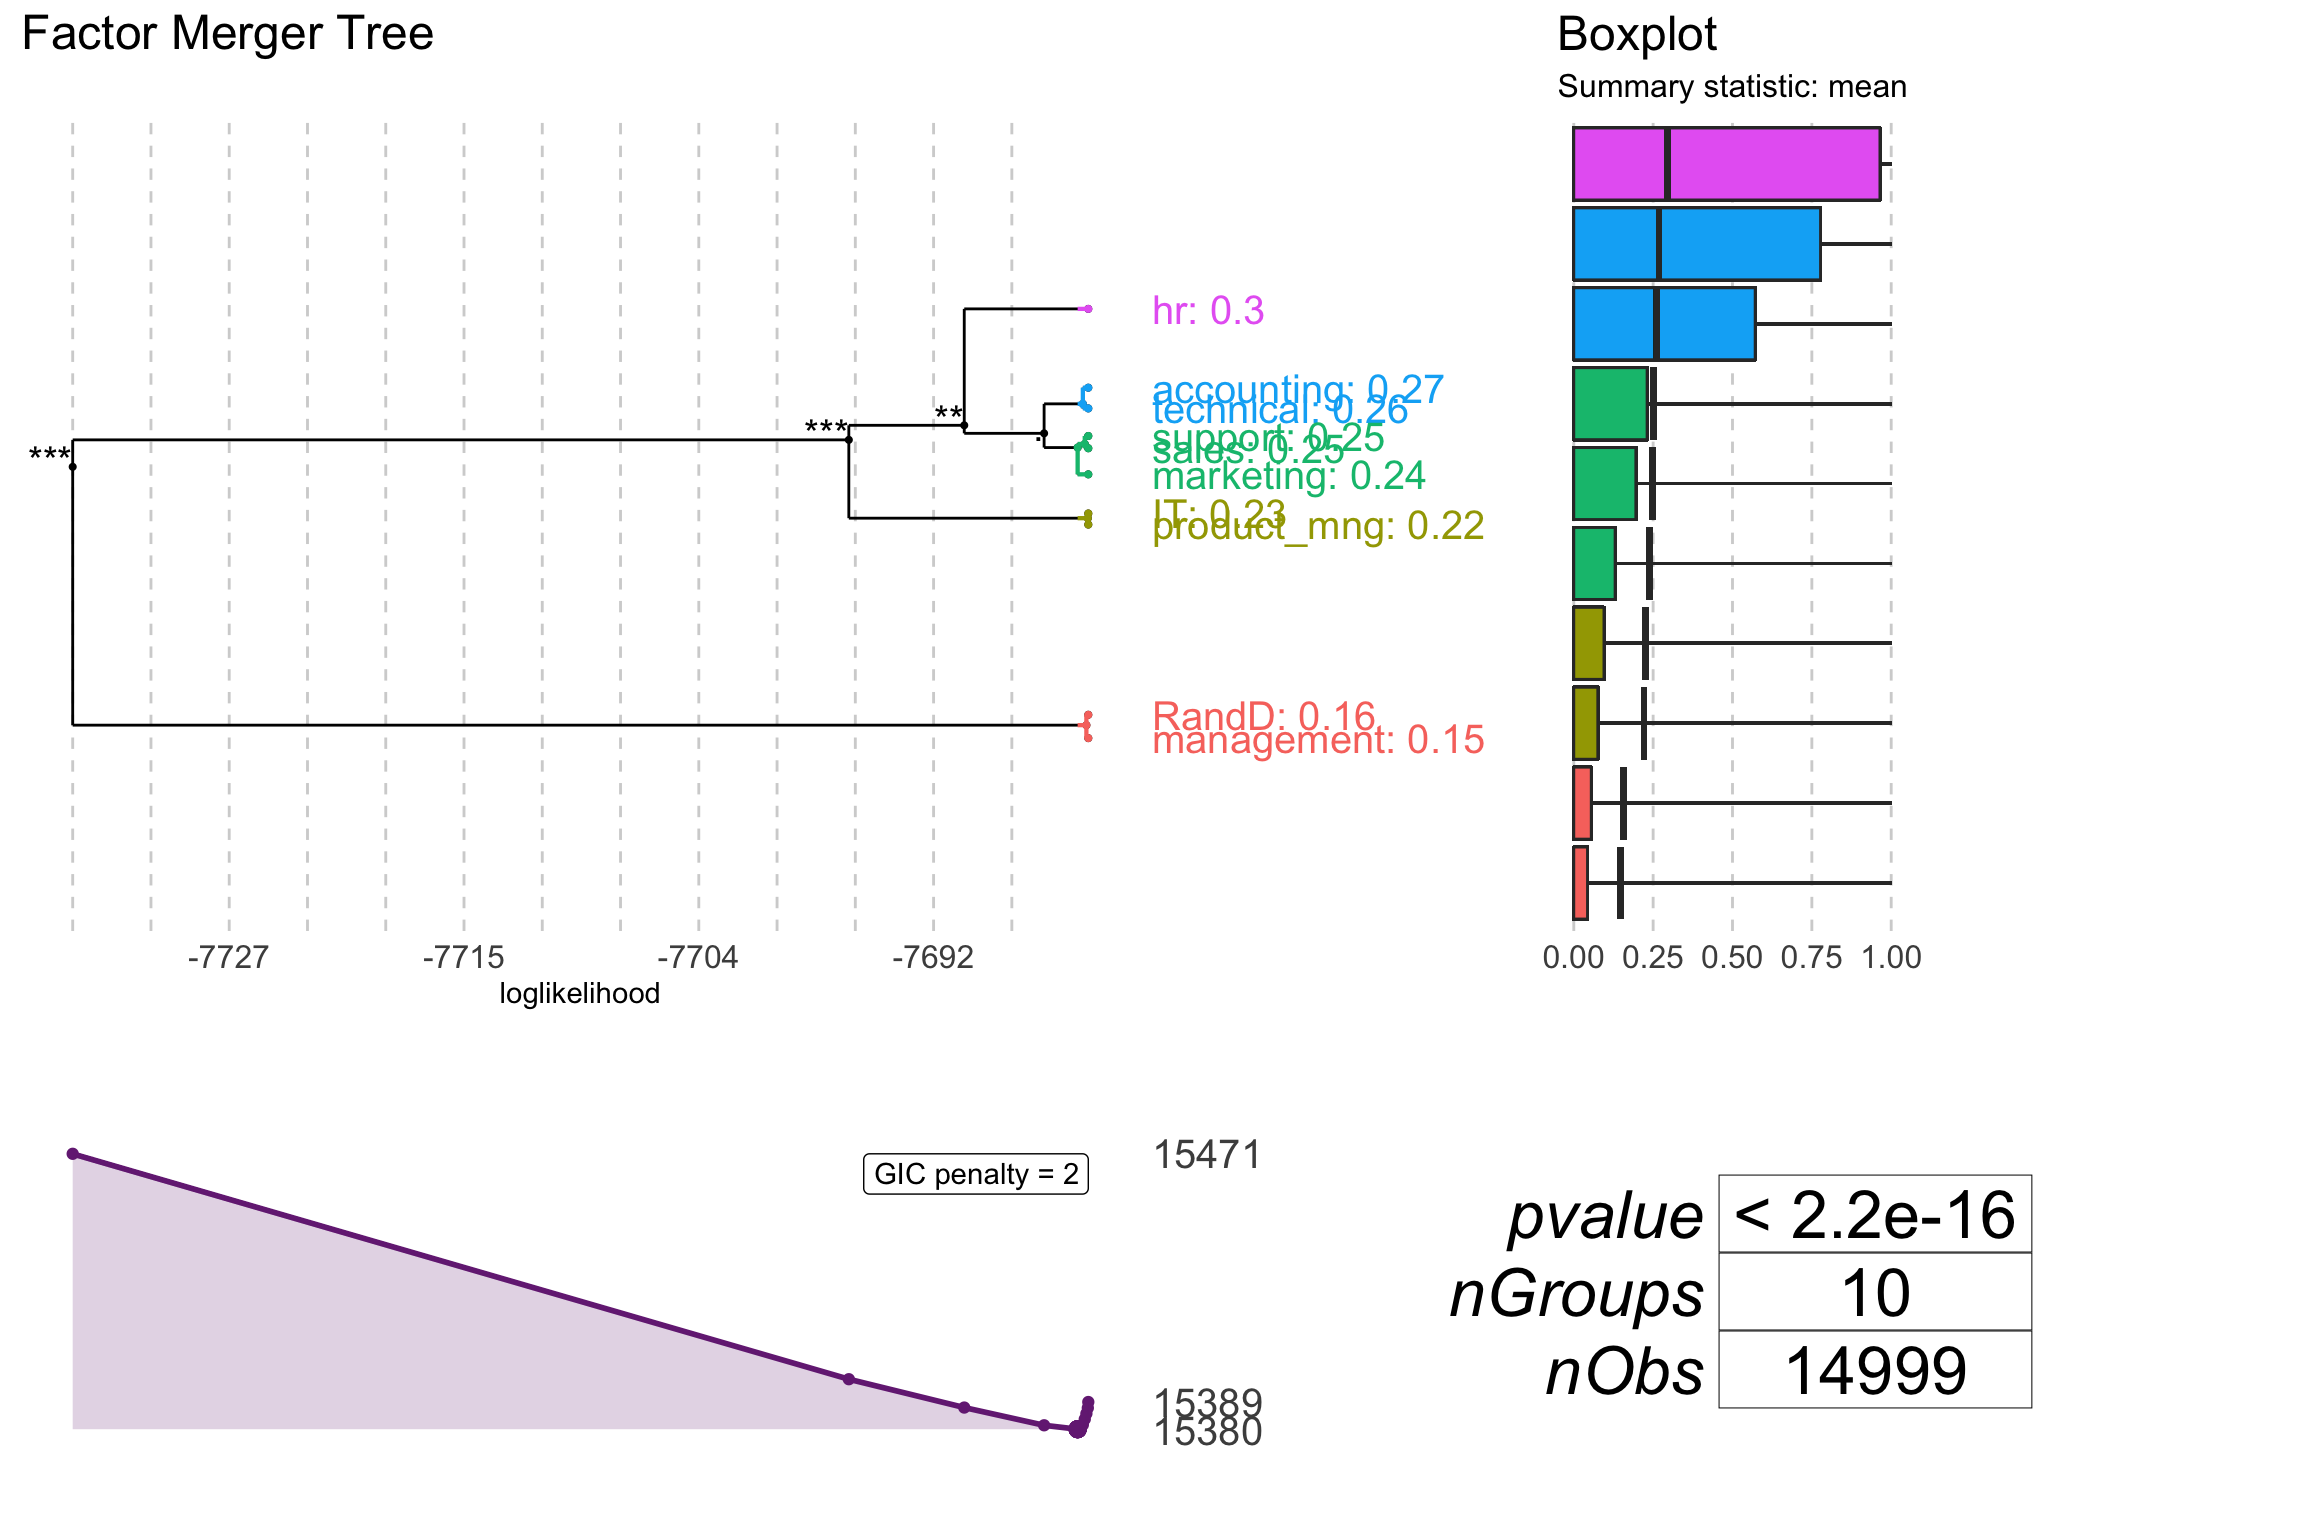
\includegraphics{DALEX_files/figure-latex/unnamed-chunk-20-1.pdf}

\begin{Shaded}
\begin{Highlighting}[]
\CommentTok{# ad0f1699de646c78a46a3bf23aeea799}
\CommentTok{# archivist::aread("pbiecek/DALEX/arepo/ad0f1699")}
\end{Highlighting}
\end{Shaded}

\subsection{Model Comparisons}\label{model-comparisons}

Marginal response plots are very useful in comparisons of different
models. Let's fit Generalized Linear Model, Random Forest Model and
XGBoost Model to the same data.

Then we can use PDP plots to compare these models. Random Forest Model
was fitted in the previous chapter. Here we are training remaining
models.

\begin{Shaded}
\begin{Highlighting}[]
\NormalTok{HR_glm_model <-}\StringTok{ }\KeywordTok{glm}\NormalTok{(left}\OperatorTok{~}\NormalTok{., }\DataTypeTok{data =}\NormalTok{ breakDown}\OperatorTok{::}\NormalTok{HR_data, }\DataTypeTok{family =} \StringTok{"binomial"}\NormalTok{)}

\KeywordTok{library}\NormalTok{(}\StringTok{"xgboost"}\NormalTok{)}
\NormalTok{model_martix_train <-}\StringTok{ }\KeywordTok{model.matrix}\NormalTok{(left}\OperatorTok{~}\NormalTok{.}\OperatorTok{-}\DecValTok{1}\NormalTok{, breakDown}\OperatorTok{::}\NormalTok{HR_data)}
\NormalTok{data_train <-}\StringTok{ }\KeywordTok{xgb.DMatrix}\NormalTok{(model_martix_train, }\DataTypeTok{label =}\NormalTok{ breakDown}\OperatorTok{::}\NormalTok{HR_data}\OperatorTok{$}\NormalTok{left)}
\NormalTok{param <-}\StringTok{ }\KeywordTok{list}\NormalTok{(}\DataTypeTok{max_depth =} \DecValTok{2}\NormalTok{, }\DataTypeTok{eta =} \DecValTok{1}\NormalTok{, }\DataTypeTok{silent =} \DecValTok{1}\NormalTok{, }\DataTypeTok{nthread =} \DecValTok{2}\NormalTok{,}
              \DataTypeTok{objective =} \StringTok{"binary:logistic"}\NormalTok{, }\DataTypeTok{eval_metric =} \StringTok{"auc"}\NormalTok{)}
\NormalTok{HR_xgb_model <-}\StringTok{ }\KeywordTok{xgb.train}\NormalTok{(param, data_train, }\DataTypeTok{nrounds =} \DecValTok{50}\NormalTok{)}
\end{Highlighting}
\end{Shaded}

Models are trained. Now we can create explainers and single variable
explanations

\begin{Shaded}
\begin{Highlighting}[]
\NormalTok{logit <-}\StringTok{ }\ControlFlowTok{function}\NormalTok{(x) }\KeywordTok{exp}\NormalTok{(x)}\OperatorTok{/}\NormalTok{(}\DecValTok{1}\OperatorTok{+}\KeywordTok{exp}\NormalTok{(x))}

\NormalTok{explainer_glm <-}\StringTok{ }\KeywordTok{explain}\NormalTok{(HR_glm_model, }\DataTypeTok{data =}\NormalTok{ HR_data)}
\NormalTok{expl_glm <-}\StringTok{ }\KeywordTok{single_variable}\NormalTok{(explainer_glm, }\StringTok{"satisfaction_level"}\NormalTok{, }\StringTok{"pdp"}\NormalTok{, }\DataTypeTok{trans=}\NormalTok{logit)}

\NormalTok{explainer_xgb <-}\StringTok{ }\KeywordTok{explain}\NormalTok{(HR_xgb_model, }\DataTypeTok{data =}\NormalTok{ model_martix_train)}
\NormalTok{expl_xgb <-}\StringTok{ }\KeywordTok{single_variable}\NormalTok{(explainer_xgb, }\StringTok{"satisfaction_level"}\NormalTok{, }\StringTok{"pdp"}\NormalTok{, }\DataTypeTok{trans=}\NormalTok{logit)}
\end{Highlighting}
\end{Shaded}

In order to compare these models it's enough to plot all of them into a
single chart.

\begin{Shaded}
\begin{Highlighting}[]
\KeywordTok{plot}\NormalTok{(expl_rf, expl_glm, expl_xgb)}
\end{Highlighting}
\end{Shaded}

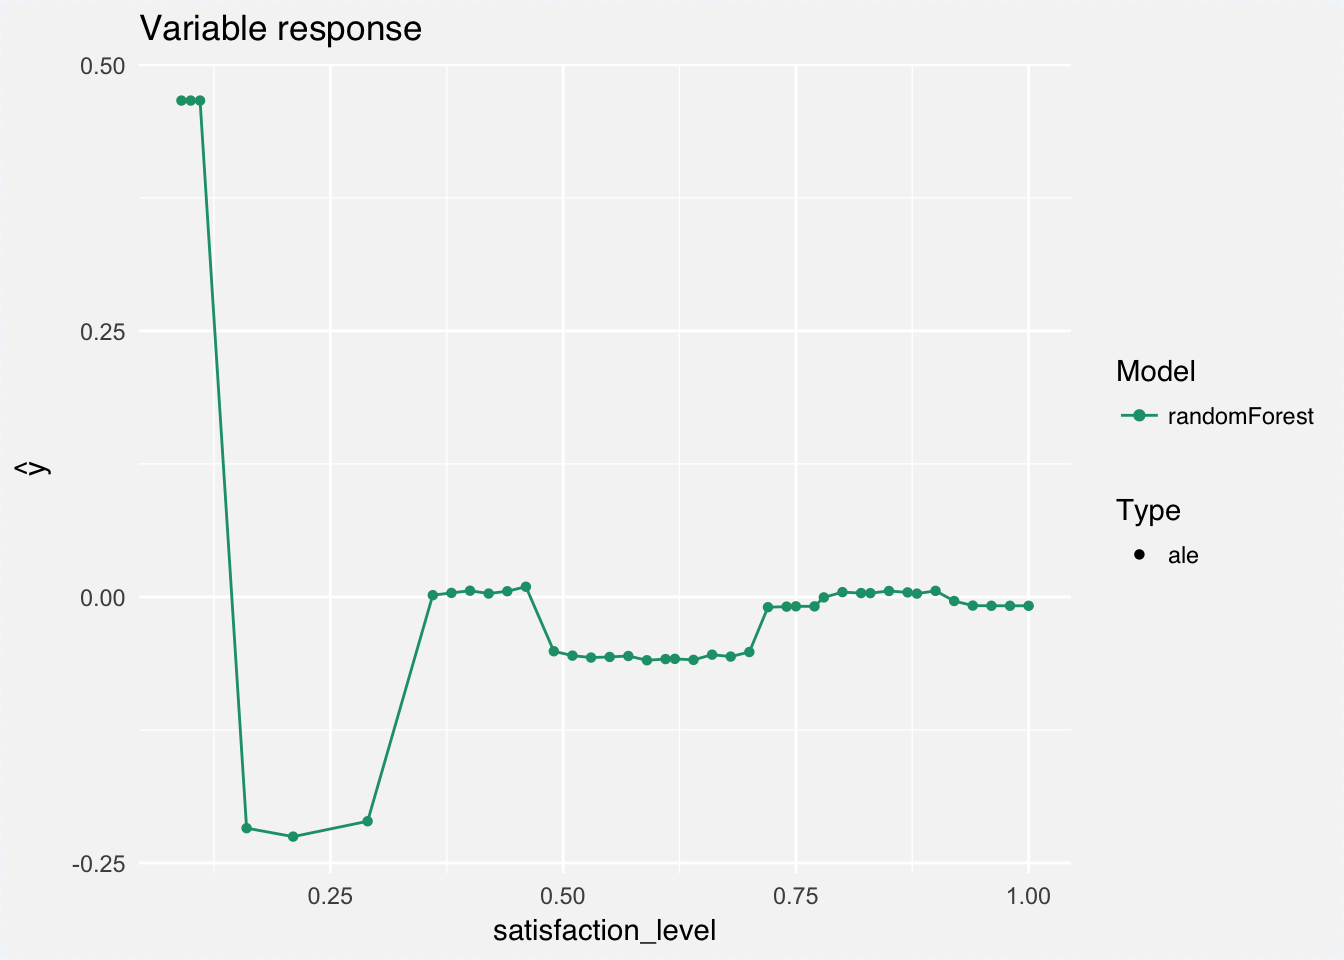
\includegraphics{DALEX_files/figure-latex/unnamed-chunk-23-1.pdf}

\section{Accumulated Local Effects
Plot}\label{accumulated-local-effects-plot}

As it is presented in the chapter @(pdpchapter), the Partial Dependence
Plot presents the expected model response with respect to marginal
distribution of \(x_{-i}\). In some cases, e.g.~when repressors are
highly correlated, expectation over the marginal distribution may lead
to biases/poorly extrapolated model responses. Especially in area far
from the training set (see \citep{ALEPlot} for more details).

Accumulated local effects (ALE) plots (see \textbf{ALEPlot} package
\citep{ALEPlot}) solves this problem by using conditional distribution
\(x_{-i}|x_i = x_i^*\). This leads to more stable and reliable estimates
(at least when the predictors are highly correlated).

Let see an example for ALE plots. We can used the model and explainer
created in steps 1-2 in the PDP chapter above.

Estimation of main effects for \texttt{satisfaction\_level} is similar
to the PDP curves. Here we are using \texttt{DALEX::single\_variable}
function that is calling \texttt{ALEPlot::ALEPlot} function to calculate
ALE curve for variable \texttt{satisfaction\_level}.

\begin{Shaded}
\begin{Highlighting}[]
\NormalTok{exel_rf  <-}\StringTok{ }\KeywordTok{single_variable}\NormalTok{(explainer_rf, }\DataTypeTok{variable =} \StringTok{"satisfaction_level"}\NormalTok{, }\DataTypeTok{type =} \StringTok{"ale"}\NormalTok{)}

\KeywordTok{plot}\NormalTok{(exel_rf)}
\end{Highlighting}
\end{Shaded}

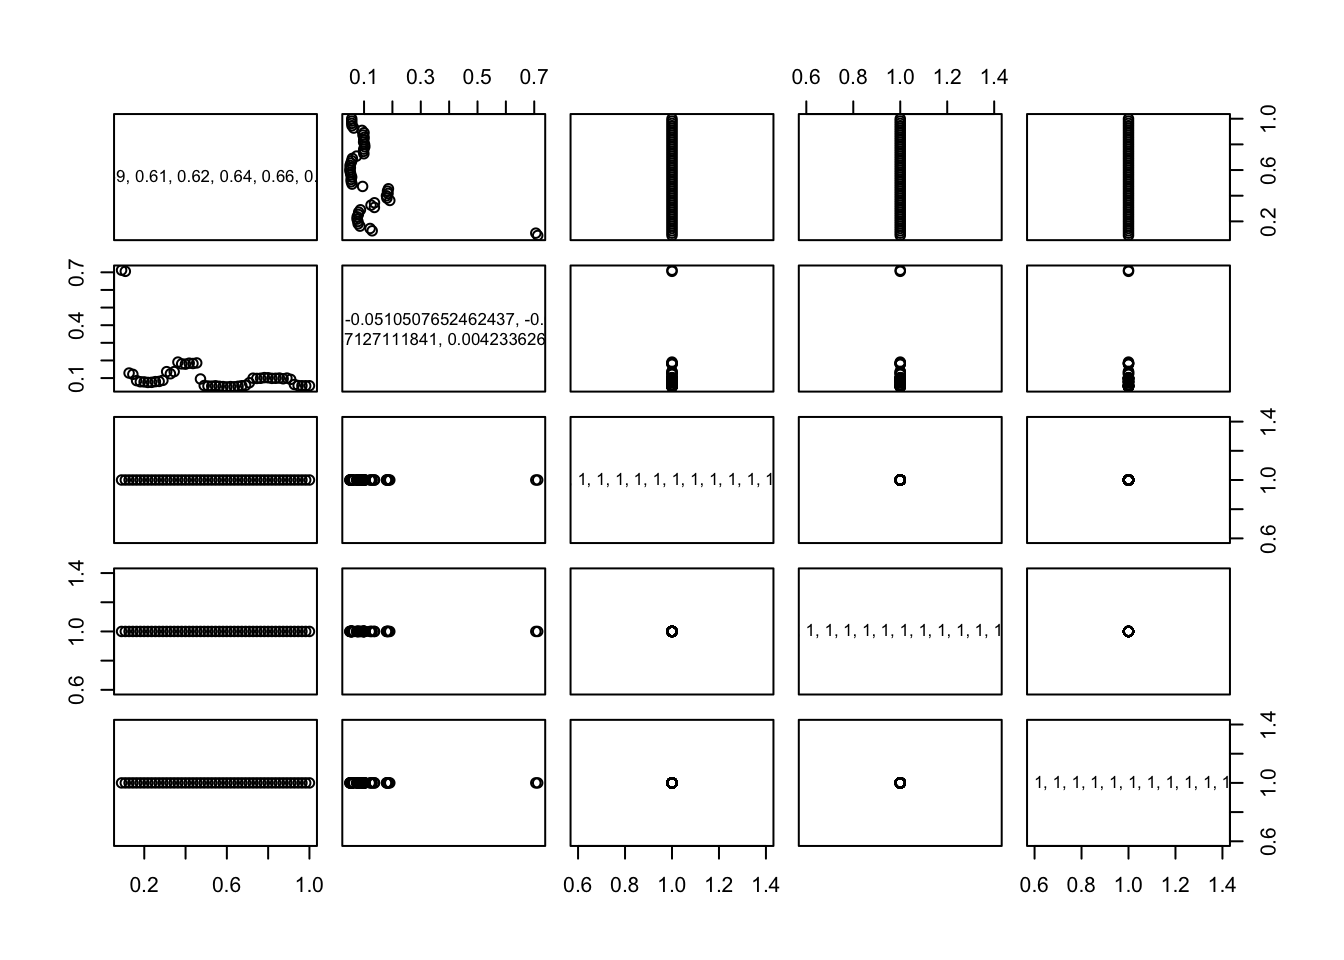
\includegraphics{DALEX_files/figure-latex/unnamed-chunk-24-1.pdf}

It may be useful to compare ALEPlots and PDP plots. Again, it's simple
with the generic DALEX function.

\begin{Shaded}
\begin{Highlighting}[]
\KeywordTok{plot}\NormalTok{(expl_rf, exel_rf)}
\end{Highlighting}
\end{Shaded}

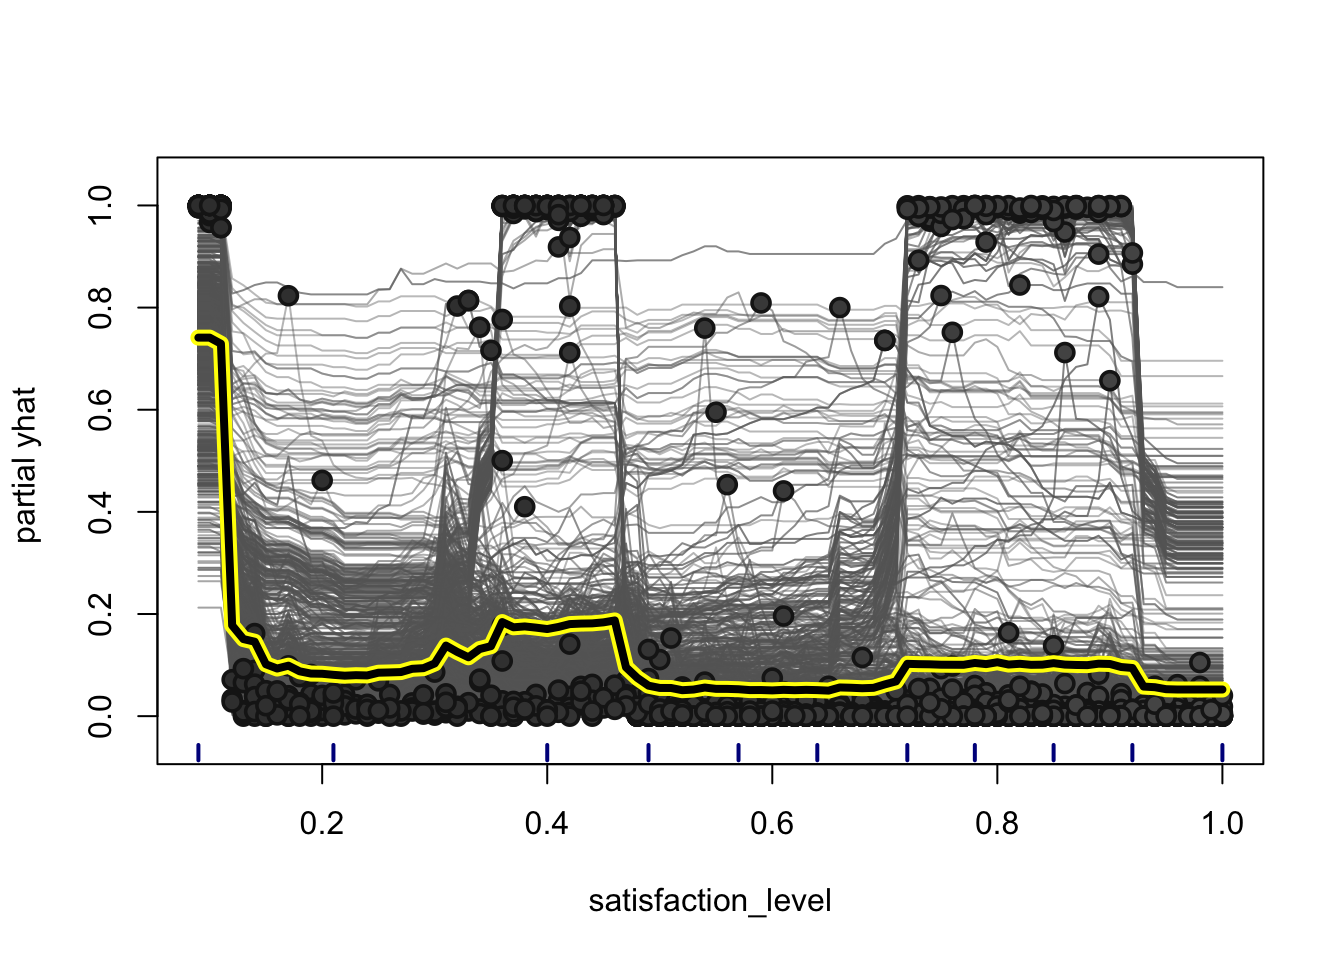
\includegraphics{DALEX_files/figure-latex/unnamed-chunk-25-1.pdf}

\section{Individual Conditional Expectation
Plot}\label{individual-conditional-expectation-plot}

Individual Conditional Expectations (ICE) may be considered as an
extension of the PDP curves (see \textbf{ICEbox} package
\citep{ICEbox}). Instead of plotting expected value over all
observations, for ICE we are plotting individual conditional model
responses. Average of ICE curves results in PDP curve.

An ICE curve for observation \(k\) over variable \(i\) may be defined as

\[
ice_k(x_i) = f(x^i, x_k^{-i}; \theta) 
\]

ICE curves can be plotted with \texttt{pdp} package. Note that curves
may be cantered in a given point, this helps in identification of
possible interactions.

\begin{Shaded}
\begin{Highlighting}[]
\KeywordTok{library}\NormalTok{(}\StringTok{"pdp"}\NormalTok{)}
\KeywordTok{library}\NormalTok{(}\StringTok{"randomForest"}\NormalTok{)}
\KeywordTok{library}\NormalTok{(}\StringTok{"breakDown"}\NormalTok{)}
\KeywordTok{library}\NormalTok{(}\StringTok{"ggplot2"}\NormalTok{)}

\NormalTok{HR_rf_model <-}\StringTok{ }\KeywordTok{randomForest}\NormalTok{(left}\OperatorTok{~}\NormalTok{., }\DataTypeTok{data =}\NormalTok{ breakDown}\OperatorTok{::}\NormalTok{HR_data, }\DataTypeTok{ntree =} \DecValTok{100}\NormalTok{)}

\NormalTok{part_rf_satisfaction <-}\StringTok{ }\KeywordTok{partial}\NormalTok{(HR_rf_model, }\StringTok{"satisfaction_level"}\NormalTok{)}

\NormalTok{part_rf_satisfaction <-}\StringTok{ }\KeywordTok{partial}\NormalTok{(HR_rf_model, }\DataTypeTok{pred.var =} \StringTok{"satisfaction_level"}\NormalTok{, }\DataTypeTok{ice =} \OtherTok{TRUE}\NormalTok{)}
\KeywordTok{plotPartial}\NormalTok{(part_rf_satisfaction, }\DataTypeTok{rug =} \OtherTok{TRUE}\NormalTok{, }\DataTypeTok{train =}\NormalTok{ HR_data, }\DataTypeTok{alpha =} \FloatTok{0.2}\NormalTok{)}
\end{Highlighting}
\end{Shaded}

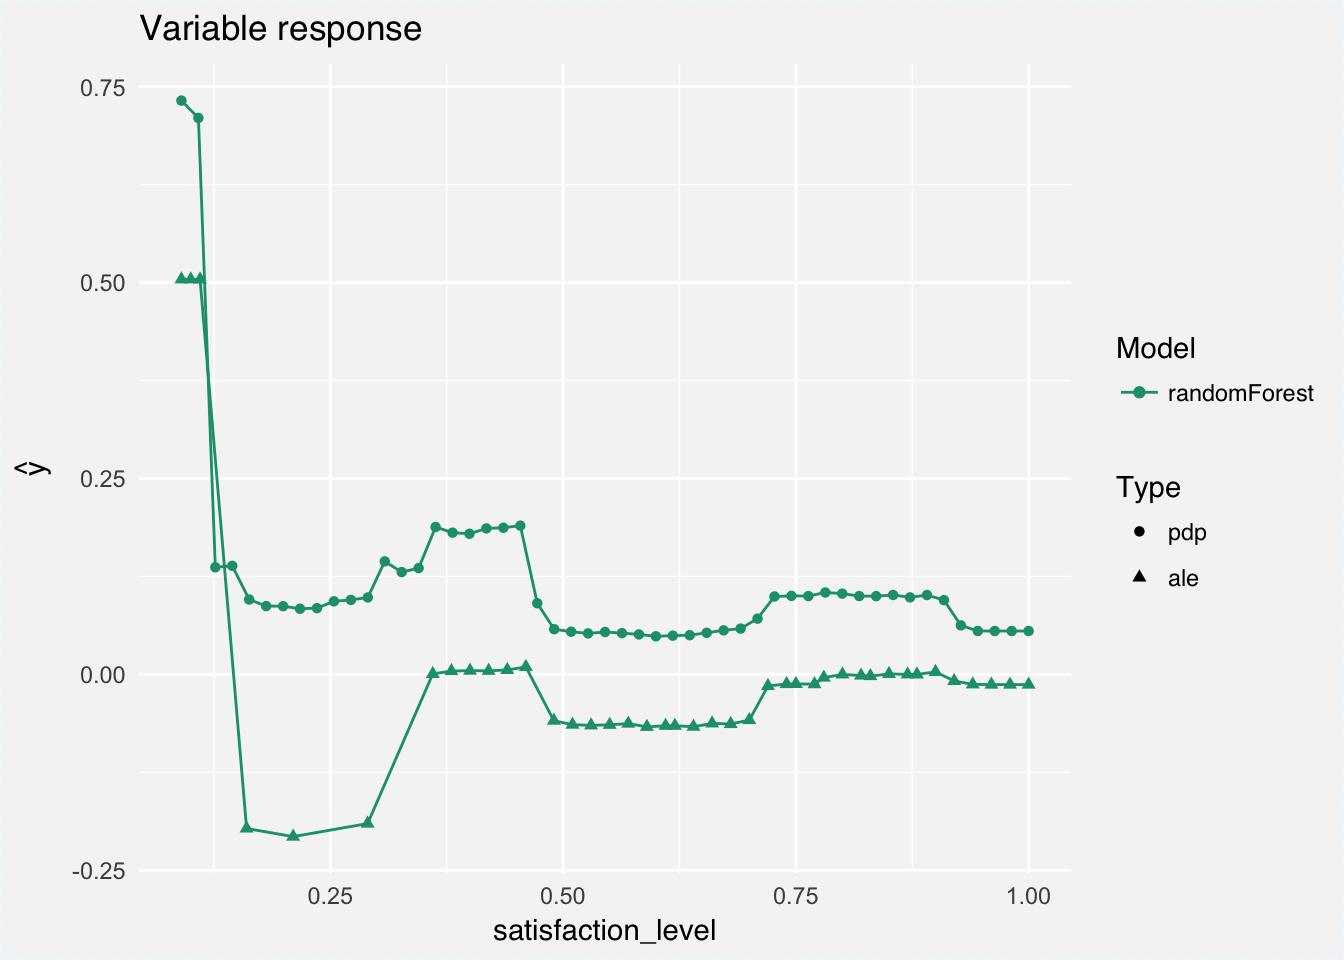
\includegraphics{DALEX_files/figure-latex/unnamed-chunk-26-1.pdf}

\begin{Shaded}
\begin{Highlighting}[]
\KeywordTok{autoplot}\NormalTok{(part_rf_satisfaction, }\DataTypeTok{center =} \OtherTok{TRUE}\NormalTok{, }\DataTypeTok{alpha =} \FloatTok{0.2}\NormalTok{, }\DataTypeTok{rug =} \OtherTok{TRUE}\NormalTok{, }\DataTypeTok{train =}\NormalTok{ HR_data)}
\end{Highlighting}
\end{Shaded}

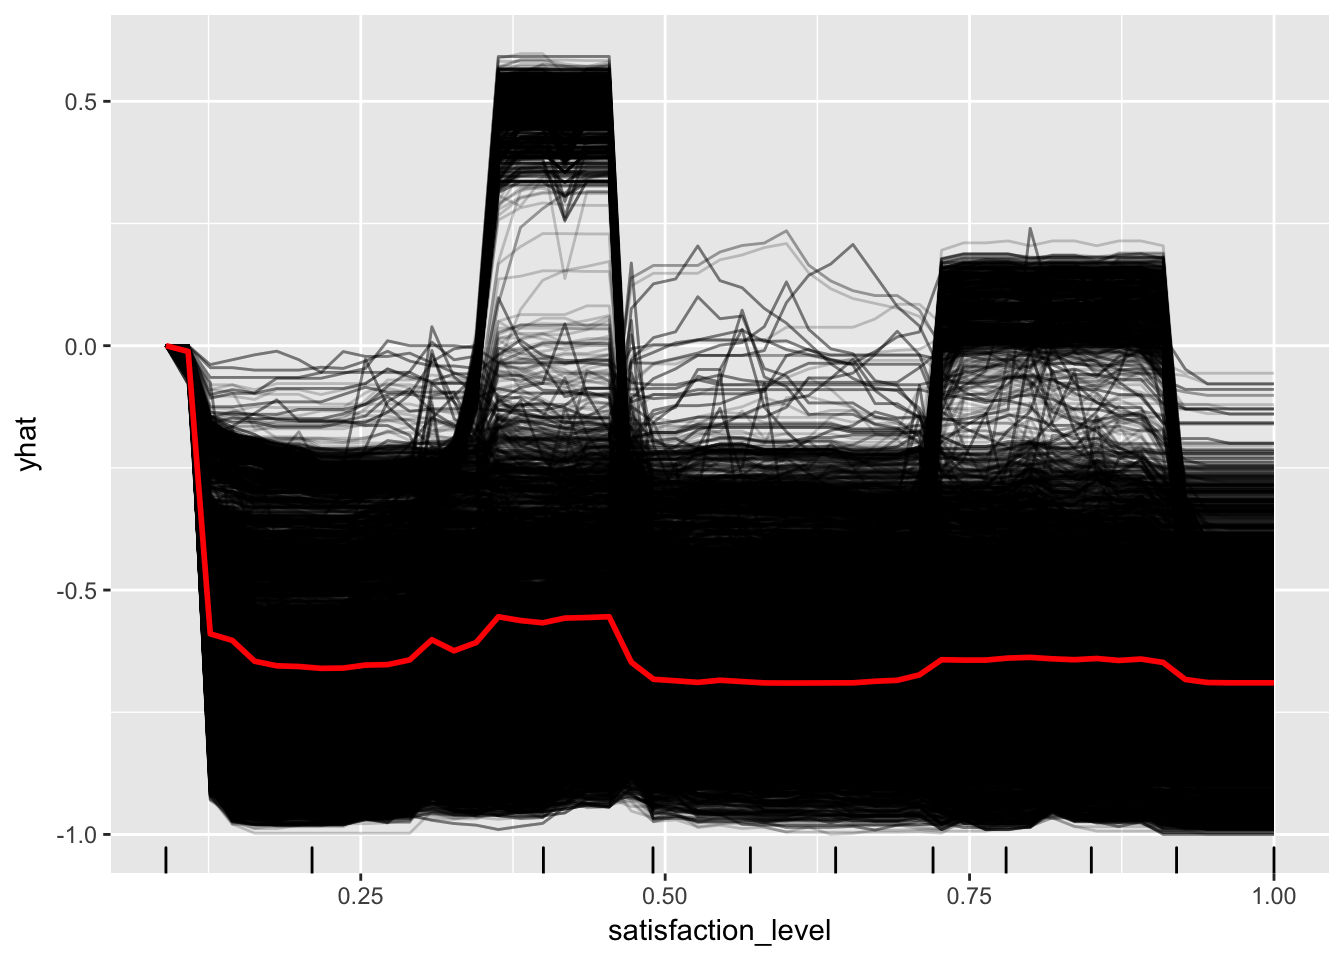
\includegraphics{DALEX_files/figure-latex/unnamed-chunk-26-2.pdf}

Or with the \texttt{ICEbox} package.

\begin{Shaded}
\begin{Highlighting}[]
\KeywordTok{library}\NormalTok{(}\StringTok{"ICEbox"}\NormalTok{)}
\NormalTok{part_rf_satisfaction =}\StringTok{ }\KeywordTok{ice}\NormalTok{(}\DataTypeTok{object =}\NormalTok{ HR_rf_model, }\DataTypeTok{X =}\NormalTok{ HR_data, }\DataTypeTok{y =}\NormalTok{ HR_data}\OperatorTok{$}\NormalTok{satisfaction_level, }
          \DataTypeTok{predictor =} \StringTok{"satisfaction_level"}\NormalTok{, }\DataTypeTok{frac_to_build =}\NormalTok{ .}\DecValTok{1}\NormalTok{)}
\end{Highlighting}
\end{Shaded}

\begin{verbatim}
## ............................................................................................
\end{verbatim}

\begin{Shaded}
\begin{Highlighting}[]
\KeywordTok{plot}\NormalTok{(part_rf_satisfaction)}
\end{Highlighting}
\end{Shaded}

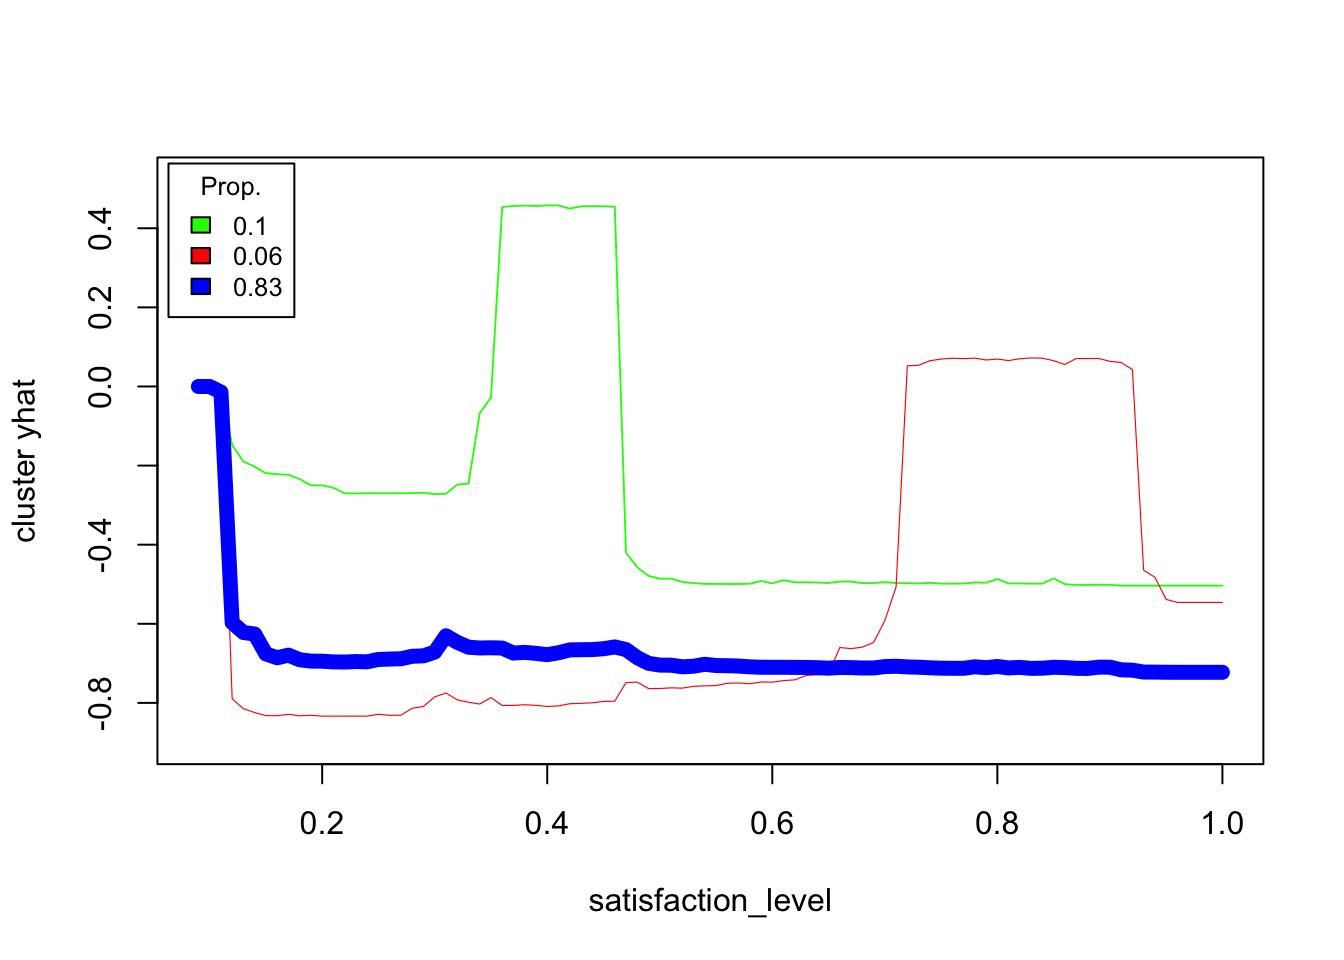
\includegraphics{DALEX_files/figure-latex/unnamed-chunk-27-1.pdf}

As ICE curves are useful tool for identification of interactions, these
individual curves may be clustered with the \texttt{clusterICE}
function.

\begin{Shaded}
\begin{Highlighting}[]
\KeywordTok{clusterICE}\NormalTok{(part_rf_satisfaction, }\DataTypeTok{nClusters =} \DecValTok{3}\NormalTok{, }\DataTypeTok{plot_legend =} \OtherTok{TRUE}\NormalTok{, }\DataTypeTok{center =} \OtherTok{TRUE}\NormalTok{)}
\end{Highlighting}
\end{Shaded}

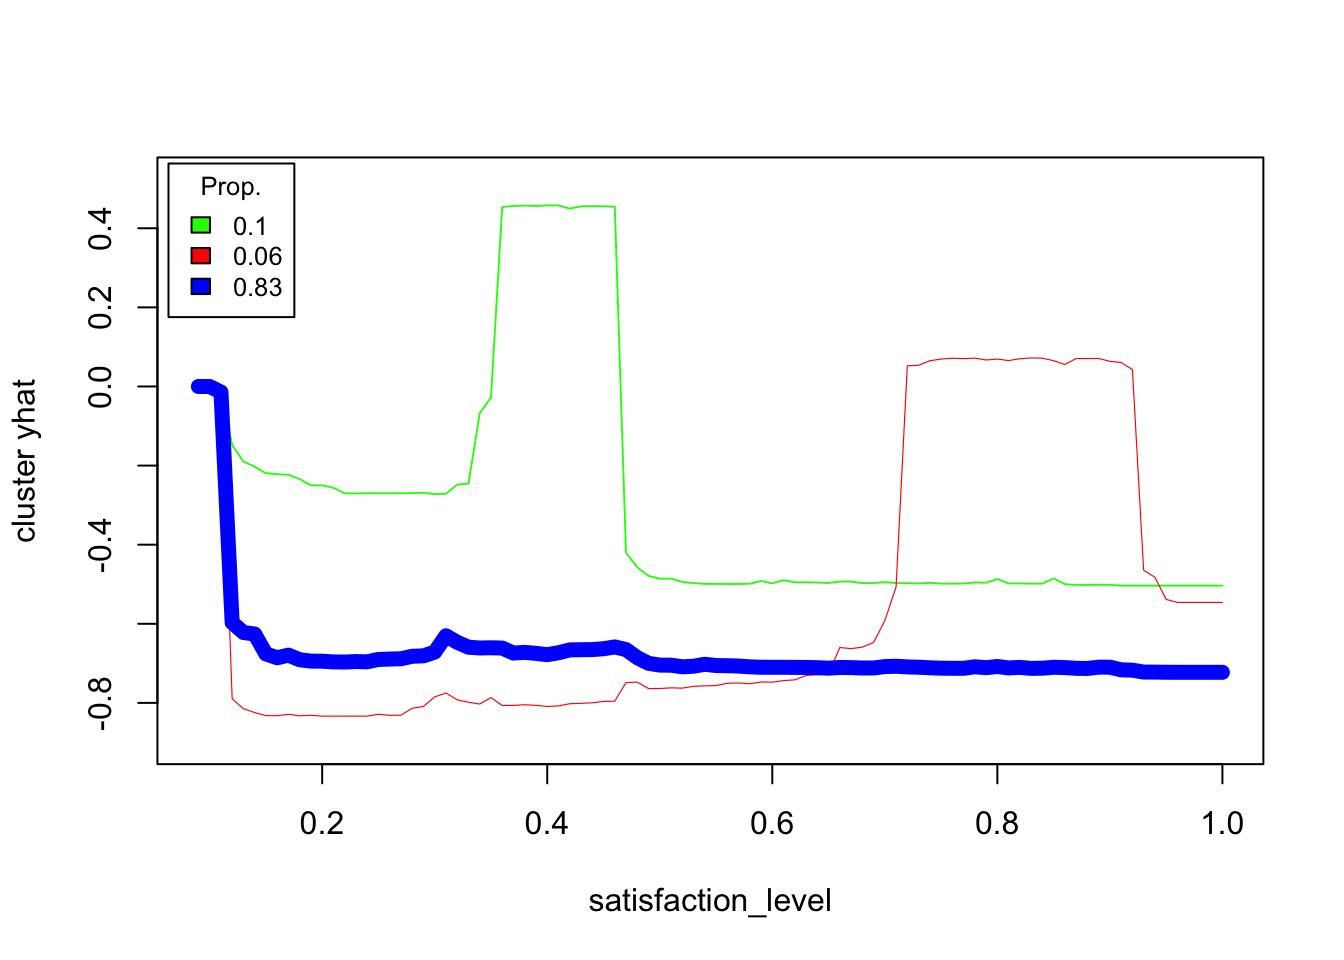
\includegraphics{DALEX_files/figure-latex/unnamed-chunk-28-1.pdf}

\section{Mering Path Plot}\label{mering-path-plot}

The package \texttt{ICEbox} is not working for factor variables while
the \texttt{pdp} package returns plots that are hard to interpret.

An interesting tool that helps to understand what is happening with
factor variables is the \textbf{factorMerger} package (see
\citep{factorMerger}).

Here we have Merging Path Plot for a factor variable \texttt{sales}.

\begin{Shaded}
\begin{Highlighting}[]
\KeywordTok{library}\NormalTok{(}\StringTok{"factorMerger"}\NormalTok{)}
\NormalTok{path <-}\StringTok{ }\KeywordTok{mergeFactors}\NormalTok{(HR_data}\OperatorTok{$}\NormalTok{left, HR_data}\OperatorTok{$}\NormalTok{sales, }\DataTypeTok{method =} \StringTok{"fast-adaptive"}\NormalTok{, }
                     \DataTypeTok{family =} \StringTok{"binomial"}\NormalTok{, }\DataTypeTok{abbreviate =} \OtherTok{FALSE}\NormalTok{)}
\KeywordTok{plot}\NormalTok{(path, }\DataTypeTok{panel =} \StringTok{"response"}\NormalTok{) }\OperatorTok{+}\StringTok{ }\KeywordTok{theme_mi2}\NormalTok{()}
\end{Highlighting}
\end{Shaded}

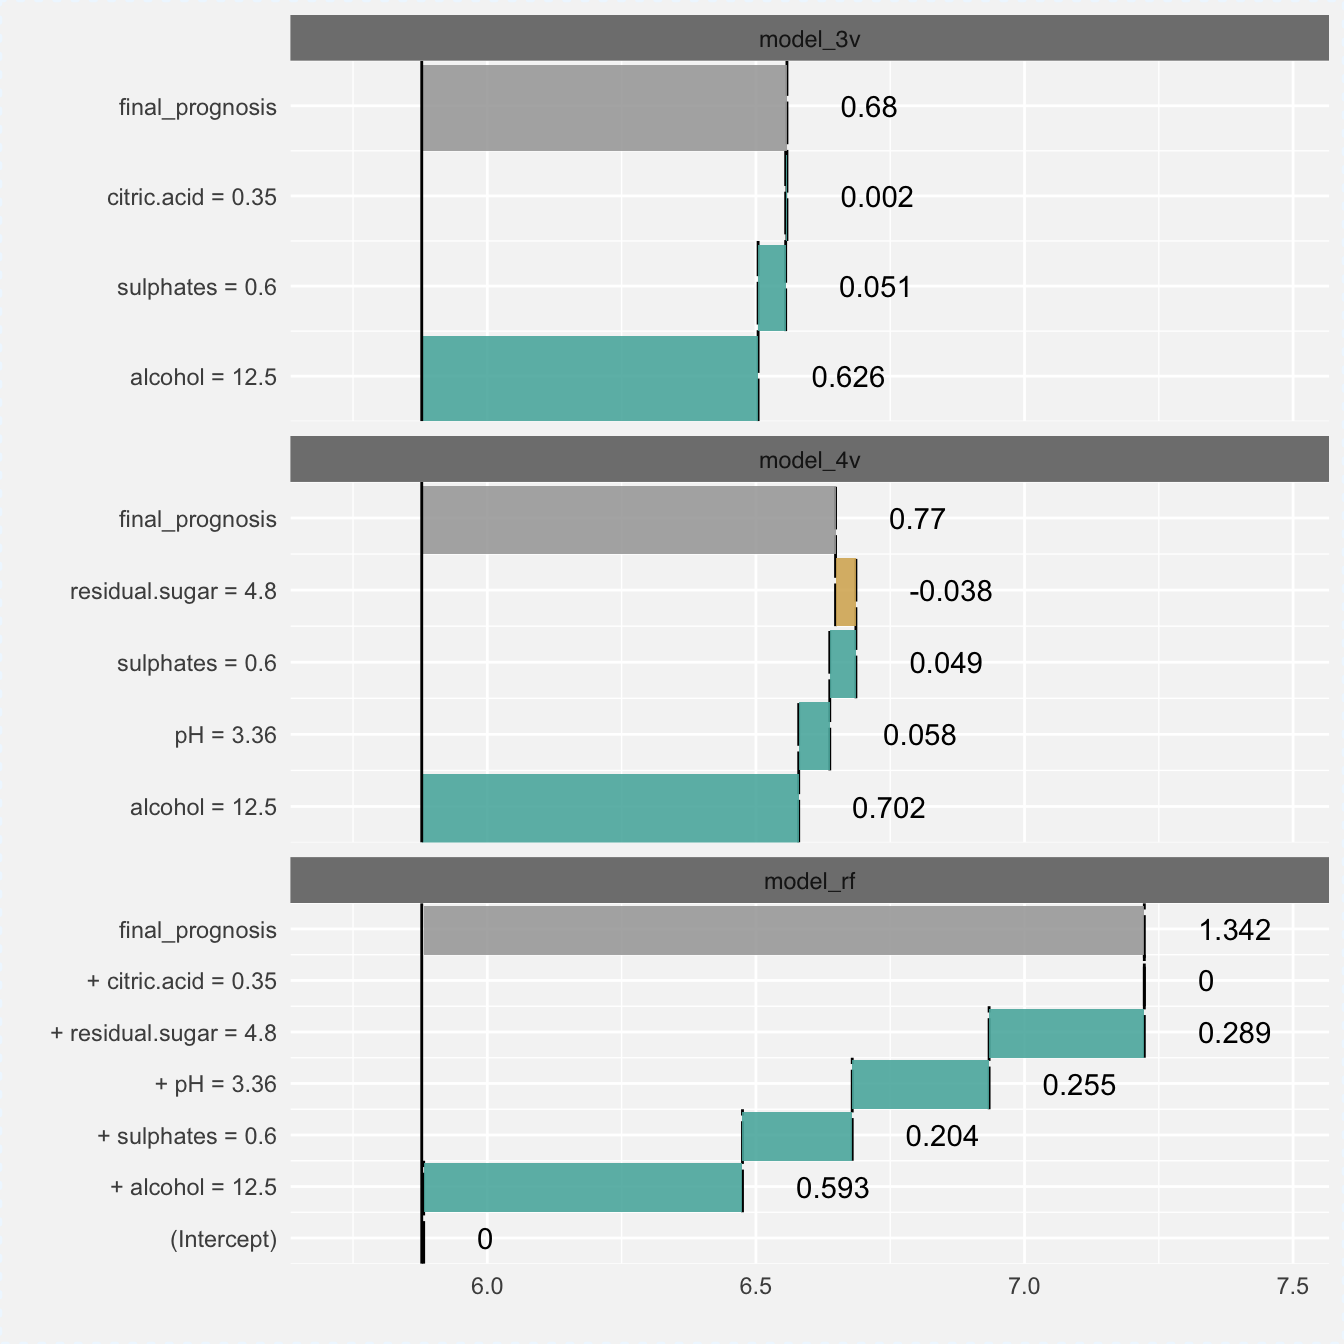
\includegraphics{DALEX_files/figure-latex/unnamed-chunk-29-1.pdf}

Note that you can use the \texttt{factorMerger} package to understand
predictions calculated with a black-box model. The random forest model
\texttt{HR\_rf\_model} returns continuous response. But the
\texttt{factorMerger} works for such variables as well.

In the top right panel one may see the distribution of predictions for
the selected group.

\begin{Shaded}
\begin{Highlighting}[]
\NormalTok{HR_data}\OperatorTok{$}\NormalTok{left_predicted <-}\StringTok{ }\KeywordTok{predict}\NormalTok{(HR_rf_model)}

\NormalTok{path <-}\StringTok{ }\KeywordTok{mergeFactors}\NormalTok{(HR_data}\OperatorTok{$}\NormalTok{left_predicted, HR_data}\OperatorTok{$}\NormalTok{sales, }\DataTypeTok{method =} \StringTok{"fast-adaptive"}\NormalTok{, }
                     \DataTypeTok{abbreviate =} \OtherTok{FALSE}\NormalTok{)}
\KeywordTok{plot}\NormalTok{(path, }\DataTypeTok{panel =} \StringTok{"response"}\NormalTok{, }\DataTypeTok{responsePanel =} \StringTok{"boxplot"}\NormalTok{, }\DataTypeTok{nodesSpacing =} \StringTok{"effects"}\NormalTok{) }\OperatorTok{+}\StringTok{ }\KeywordTok{theme_mi2}\NormalTok{()}
\end{Highlighting}
\end{Shaded}

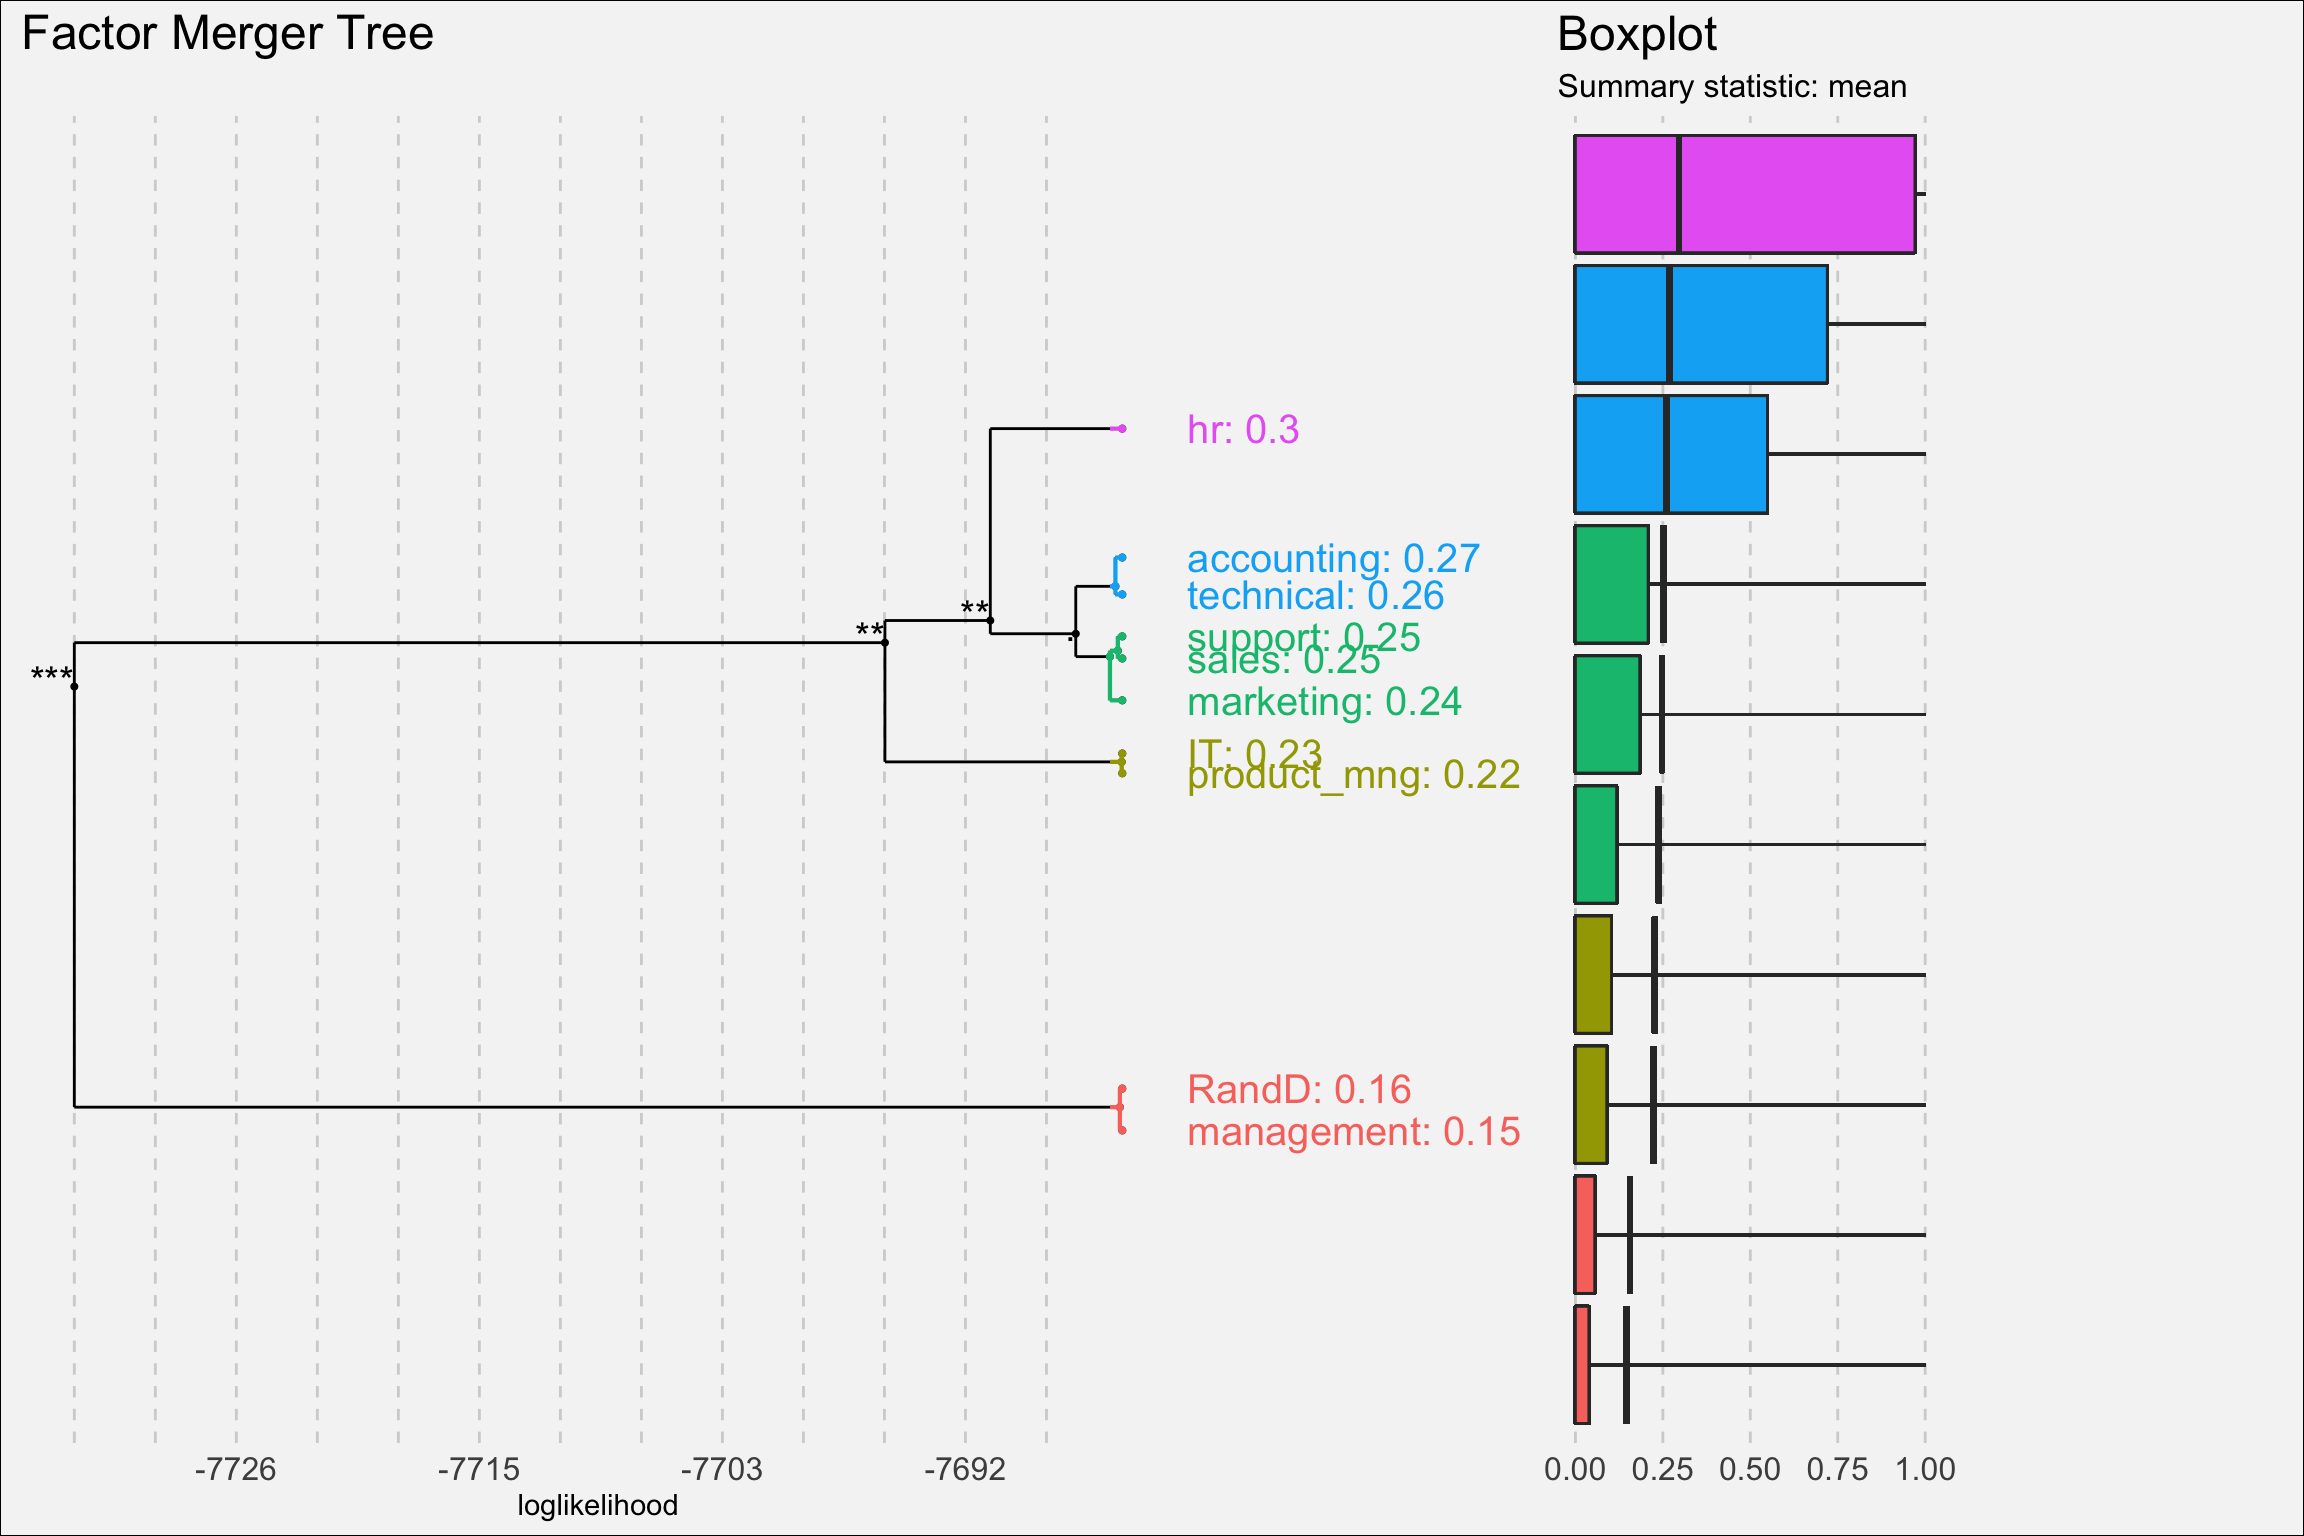
\includegraphics{DALEX_files/figure-latex/unnamed-chunk-30-1.pdf}

\chapter{Local structure}\label{local-structure}

Explainers presented in this chapter are designed to better understand
the local structure of a black box in a single point. Example
applications:

\begin{itemize}
\tightlist
\item
  explanations for predictions. Can be used to validate if a specific
  prediction is not accidental, is it based on variables important in
  the domain.
\item
  examination of curvature around a specific point (single observation).
  Can be used to determine the strength of influence onto a final model.
  Is it an outlier?
\end{itemize}

There are more interesting applications. Find out some of them in the
\emph{Why Should I Trust You?} article \citep{lime}.

\section{Basics}\label{basics}

Most ML algorithms do not learn from mistakes. One calculates
predictions and there is no room for improvement.

But! The local predictions can change that! Understanding what causes
wrong decisions may lead to model improvements. After all, if our
prediction is wrong we shall update the model.

\section{Local Interpretable (Model-agnostic) Visual
Explanations}\label{local-interpretable-model-agnostic-visual-explanations}

\begin{figure}
\centering
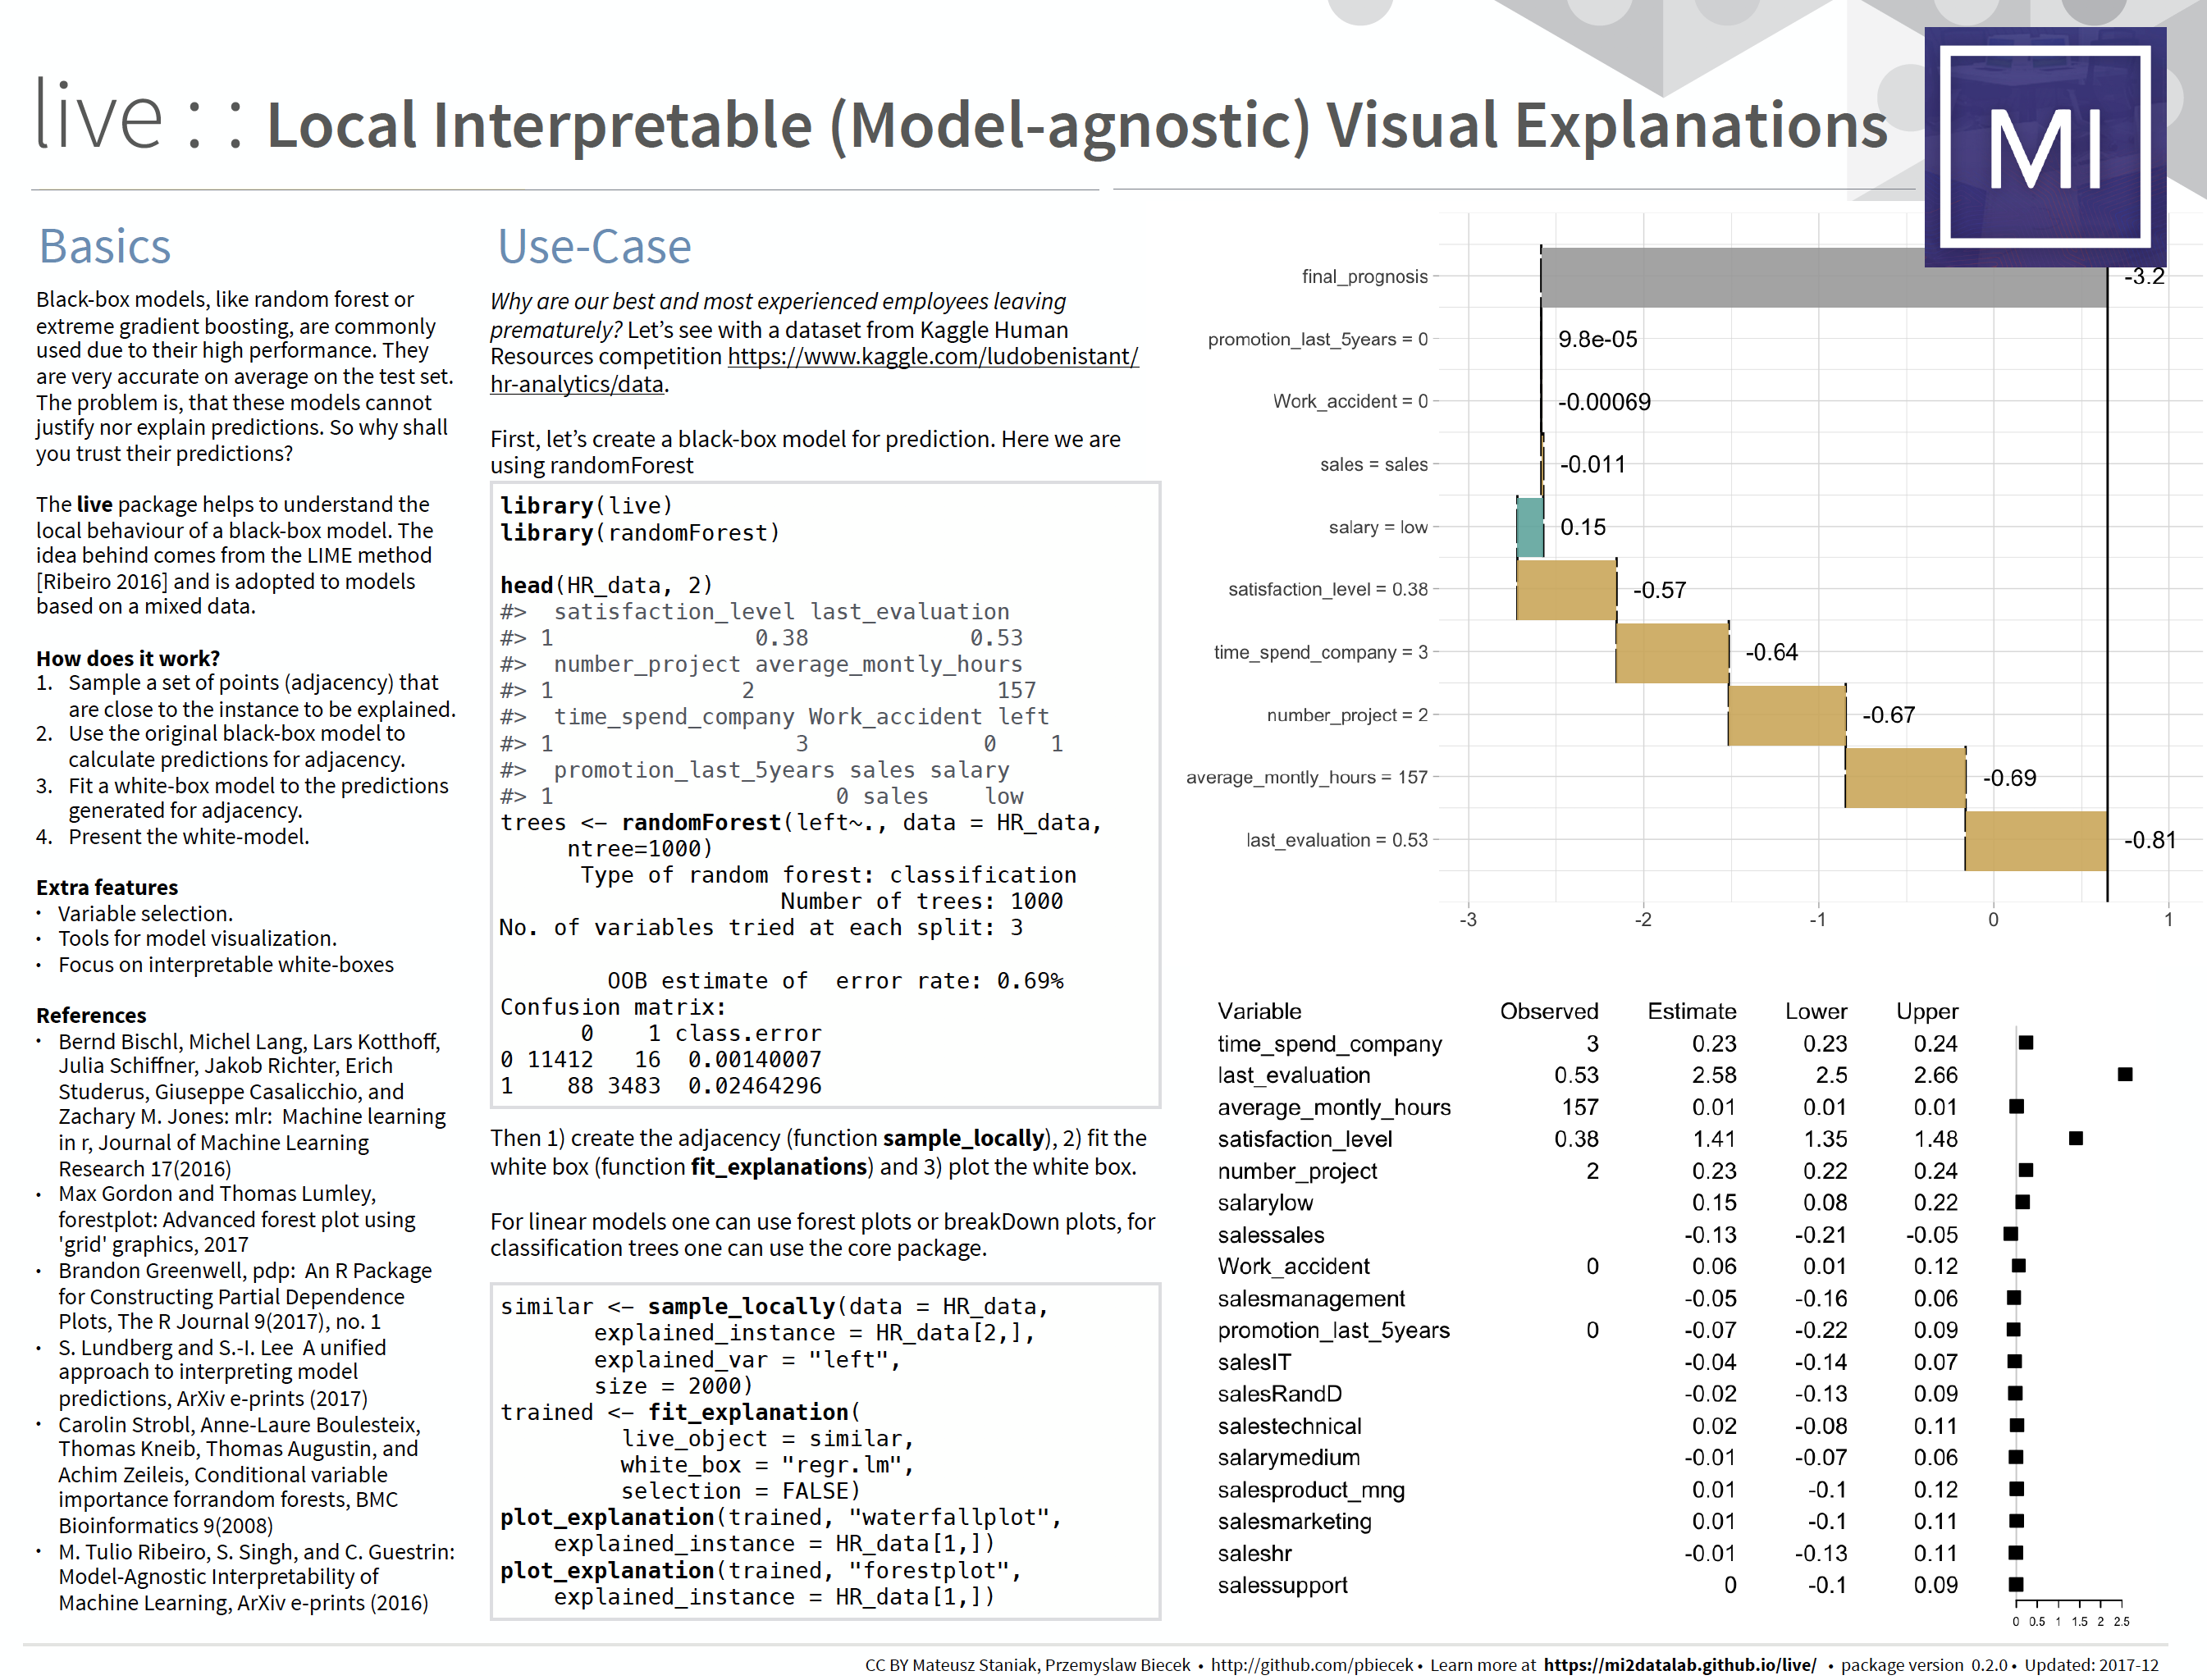
\includegraphics{images/DALEX_live.png}
\caption{Cheatsheet}
\end{figure}

The \textbf{live} package (see \citep{live}) may be seen as an extension
of the lime method (see \citep{lime}). It is based on \textbf{mlr}
general framework for training of machine learning models (see more
\citep{mlr}).

Let's see an example. We will use the \texttt{HR\_rf\_model} trained
with the \textbf{randomForest} package on Human Resources Analytics
data.

Around a selected point we will fit a linear model.

\begin{Shaded}
\begin{Highlighting}[]
\KeywordTok{library}\NormalTok{(}\StringTok{"live"}\NormalTok{)}
\KeywordTok{library}\NormalTok{(}\StringTok{"randomForest"}\NormalTok{)}
\KeywordTok{library}\NormalTok{(}\StringTok{"breakDown"}\NormalTok{)}

\NormalTok{HR_data}\OperatorTok{$}\NormalTok{left <-}\StringTok{ }\KeywordTok{as.numeric}\NormalTok{(}\KeywordTok{as.character}\NormalTok{(HR_data}\OperatorTok{$}\NormalTok{left))}

\NormalTok{HR_rf_model <-}\StringTok{ }\KeywordTok{randomForest}\NormalTok{(left}\OperatorTok{~}\NormalTok{., }\DataTypeTok{data =}\NormalTok{ HR_data,}
\DataTypeTok{ntree=}\DecValTok{100}\NormalTok{)}

\NormalTok{similar <-}\StringTok{ }\KeywordTok{sample_locally}\NormalTok{(}\DataTypeTok{data =}\NormalTok{ HR_data, }\DataTypeTok{explained_instance =}\NormalTok{ HR_data[}\DecValTok{1}\NormalTok{,], }\DataTypeTok{explained_var =} \StringTok{"left"}\NormalTok{, }\DataTypeTok{size =} \DecValTok{2000}\NormalTok{)}
\NormalTok{similar <-}\StringTok{ }\KeywordTok{add_predictions}\NormalTok{(HR_data, similar, HR_rf_model)}
\NormalTok{trained <-}\StringTok{ }\KeywordTok{fit_explanation}\NormalTok{( }\DataTypeTok{live_object =}\NormalTok{ similar, }\DataTypeTok{white_box =} \StringTok{"regr.lm"}\NormalTok{, }\DataTypeTok{selection =} \OtherTok{FALSE}\NormalTok{)}
\end{Highlighting}
\end{Shaded}

Fitted model may be plotted with \emph{waterfall plot} \ldots{}

\begin{Shaded}
\begin{Highlighting}[]
\KeywordTok{plot_explanation}\NormalTok{(trained, }\StringTok{"waterfallplot"}\NormalTok{, }\DataTypeTok{explained_instance =}\NormalTok{ HR_data[}\DecValTok{1}\NormalTok{,])}
\end{Highlighting}
\end{Shaded}

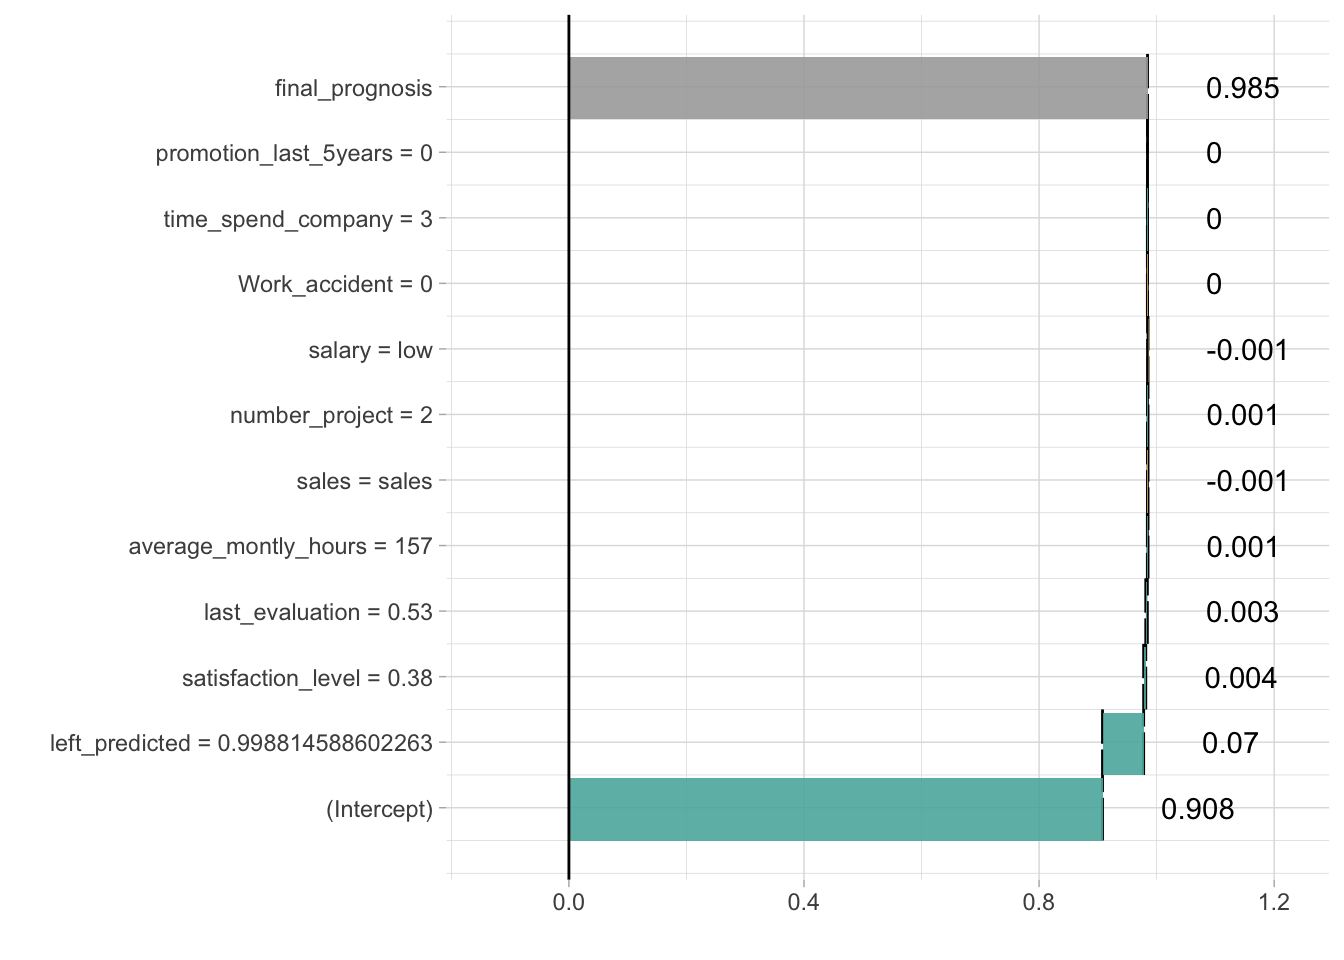
\includegraphics{DALEX_files/figure-latex/live_water-1.pdf}

\ldots{} or \emph{forest plot} \ldots{}

\begin{Shaded}
\begin{Highlighting}[]
\KeywordTok{plot_explanation}\NormalTok{(trained, }\StringTok{"forestplot"}\NormalTok{, }\DataTypeTok{explained_instance =}\NormalTok{ HR_data[}\DecValTok{1}\NormalTok{,])}
\end{Highlighting}
\end{Shaded}

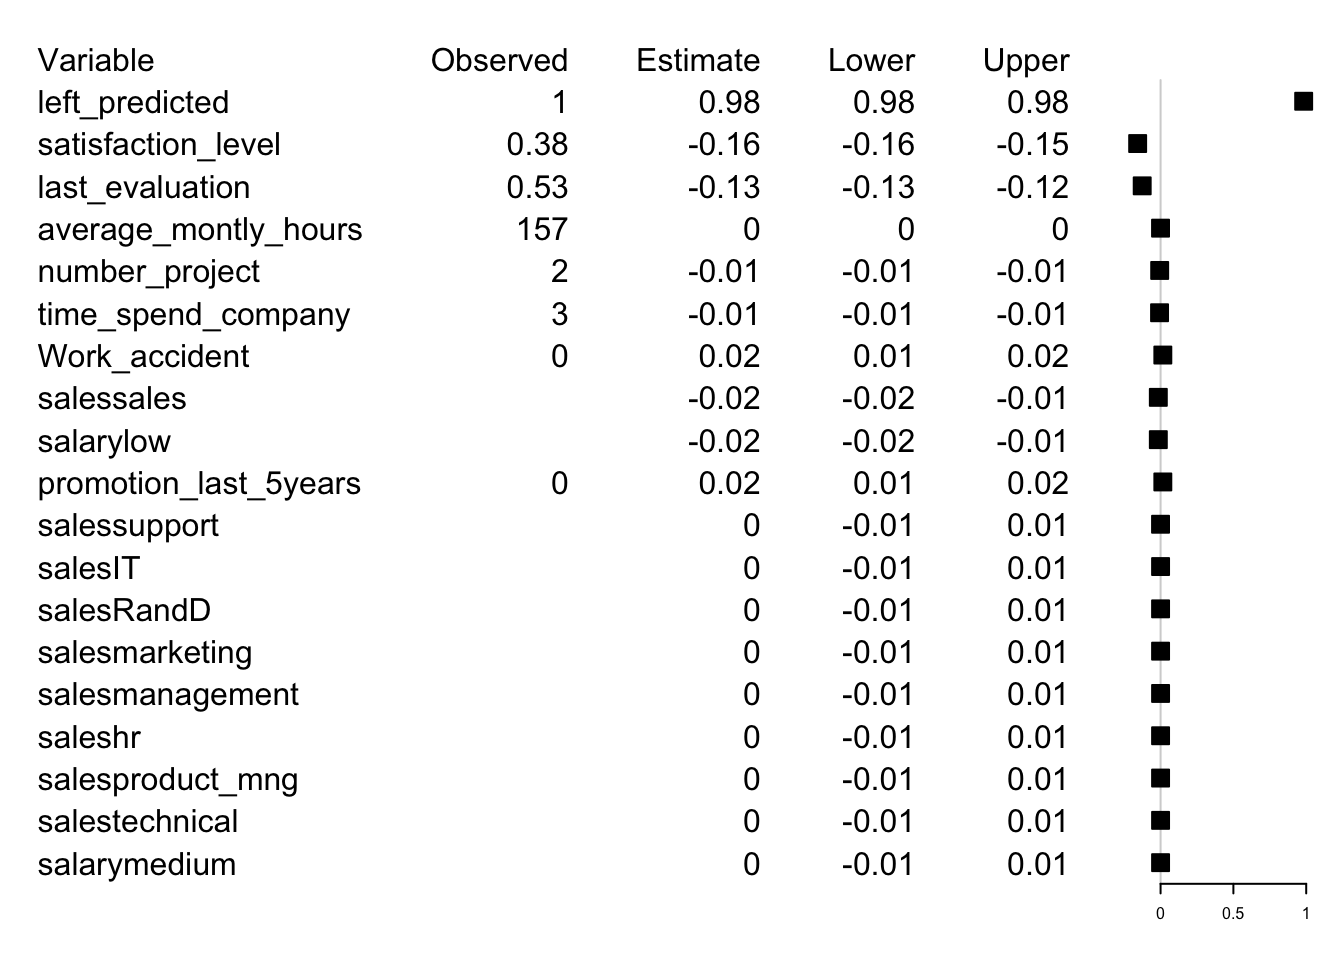
\includegraphics{DALEX_files/figure-latex/live_forest-1.pdf}

For more details consult the following vignette.

\section{breakDown}\label{breakdown}

\begin{figure}
\centering
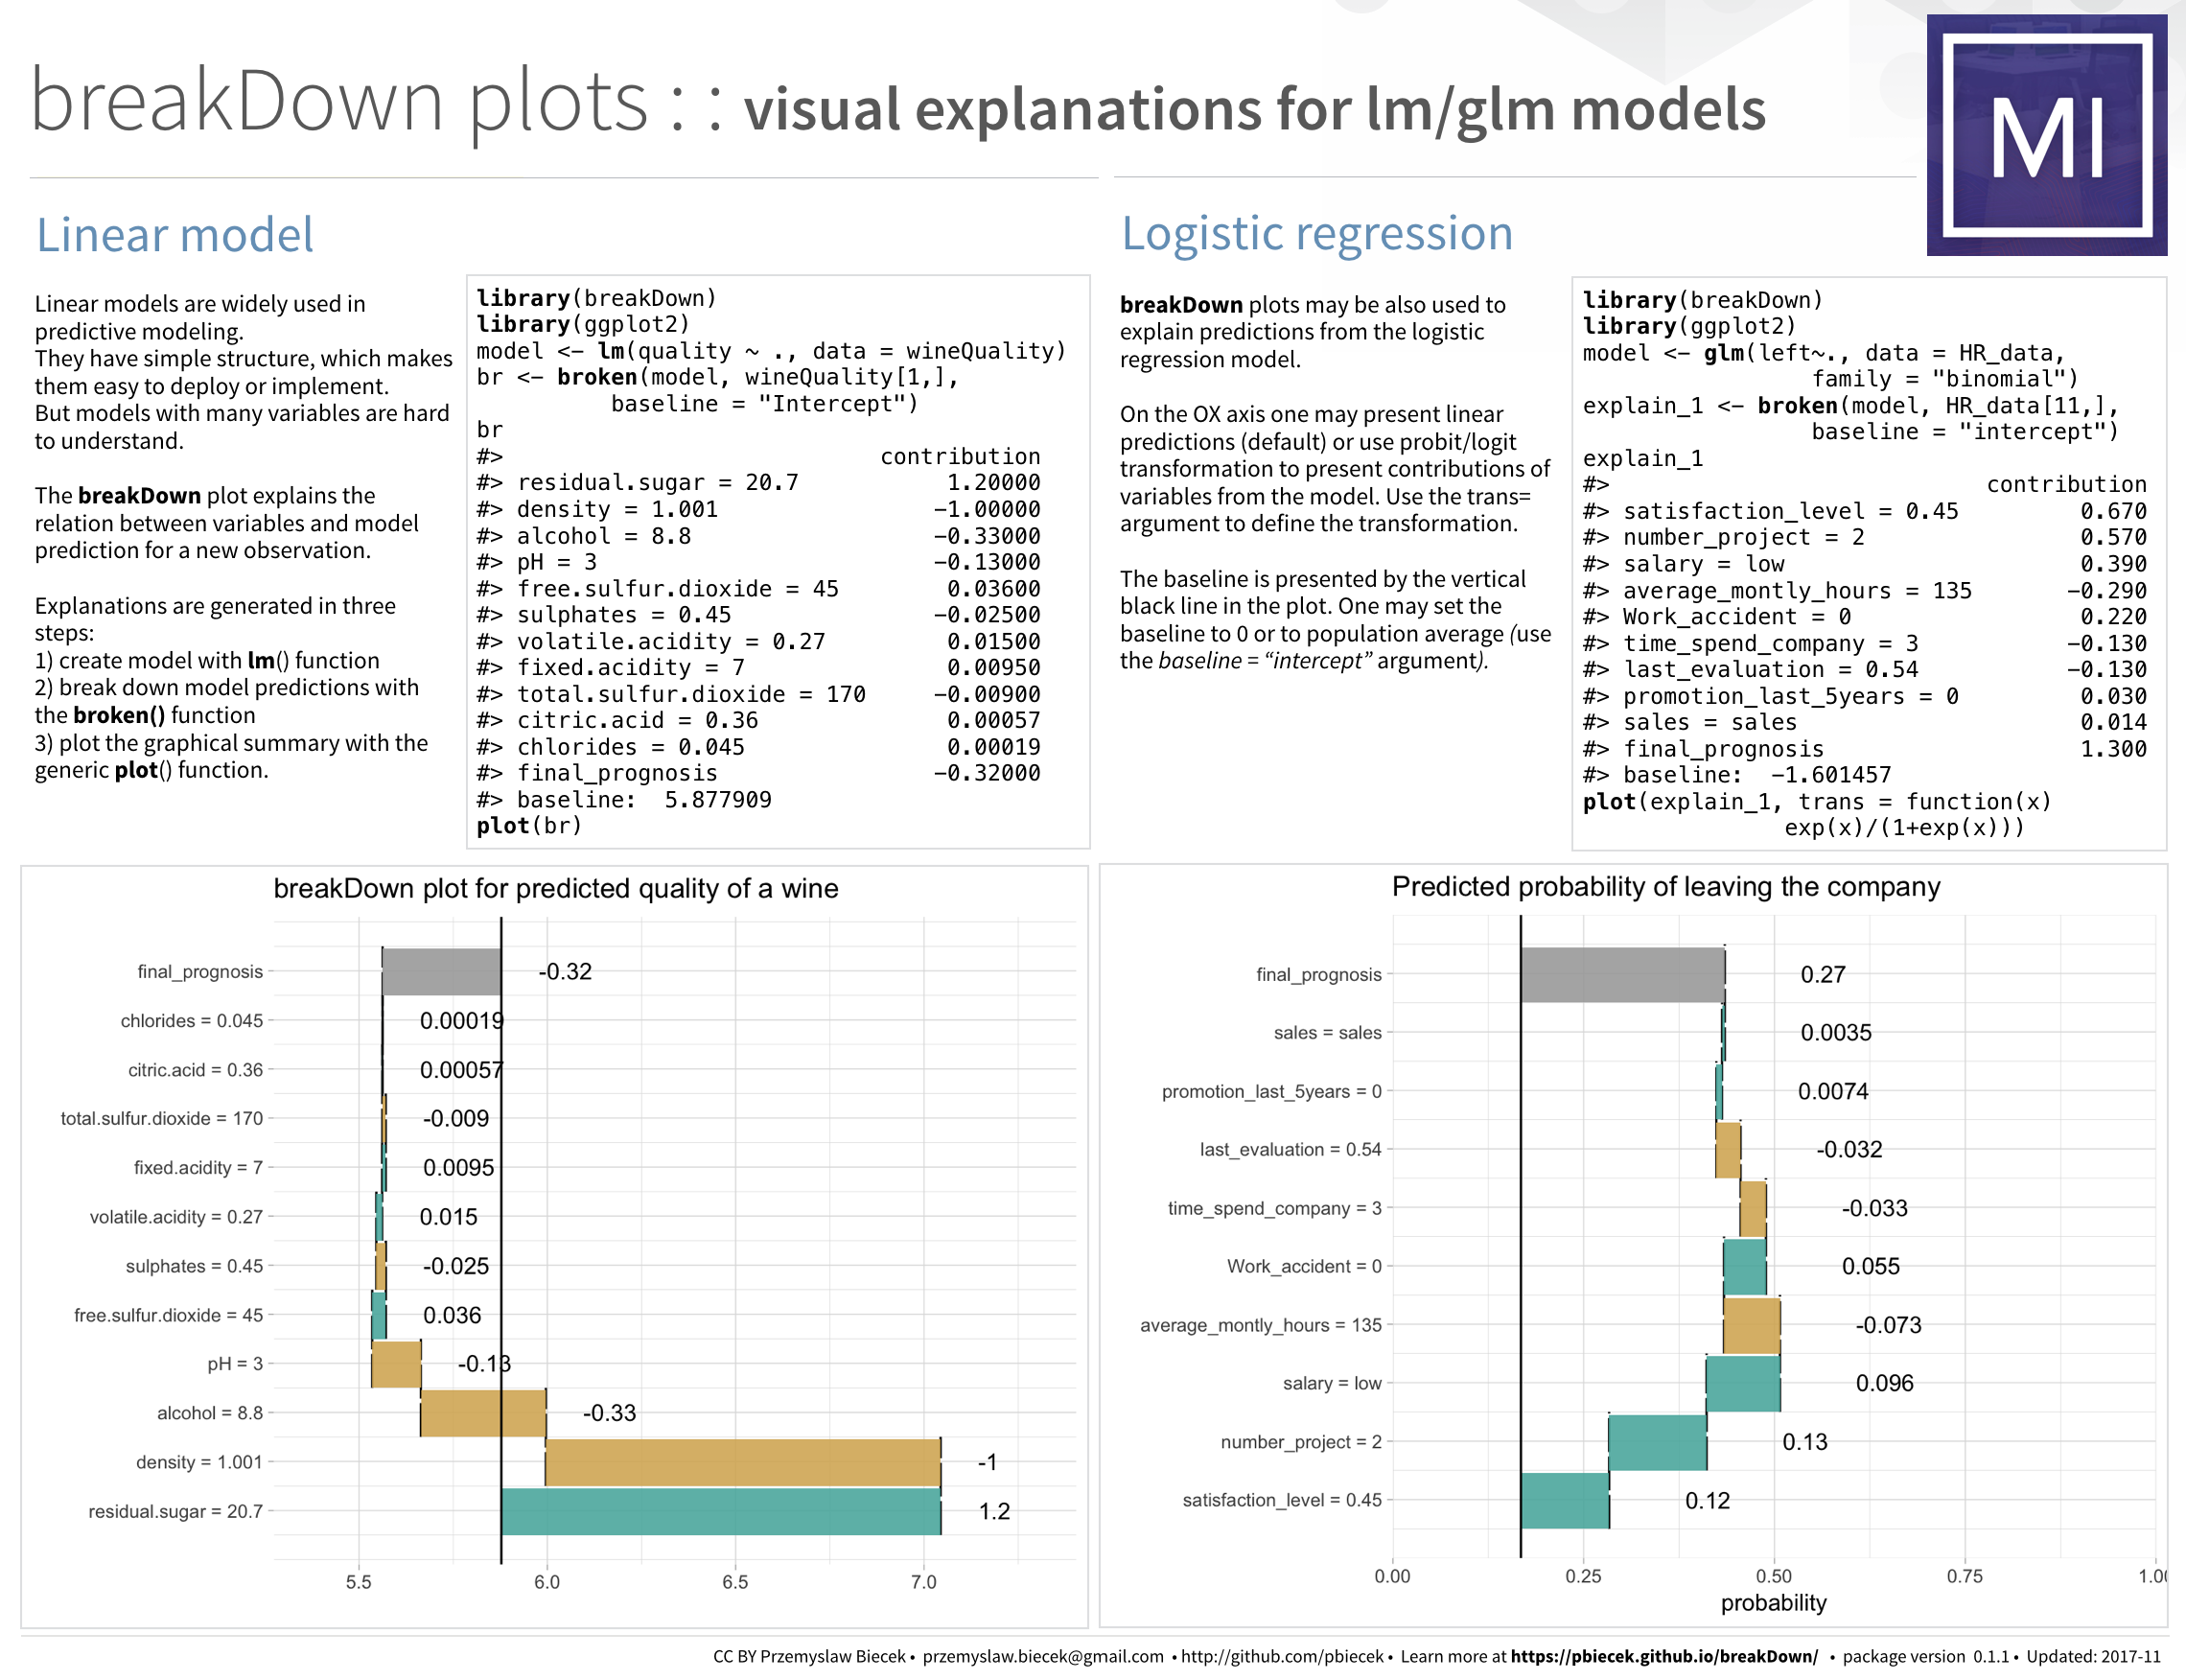
\includegraphics{images/DALEX_breakDown.png}
\caption{Cheatsheet}
\end{figure}

The \texttt{breakDown} package \citep{breakDown} explains components of
model prediction for a single observation. Right now it's working for
\texttt{lm} and \texttt{glm} models. Break Down Plots are inspired by
waterfall plots as in
\href{https://github.com/AppliedDataSciencePartners/xgboostExplainer}{\texttt{xgboostExplainer}
package}.

Break Down Plots show the contribution of every variable present in the
model.

Let's see a use case for the \texttt{wine} dataset.

The problem that we are going to solve is to create a model that
predicts wine quality and then use the model and explain it's prediction
for a single wine.

We start with a linear Gaussian model for \texttt{quality} with three
dependent variables \texttt{citric.acid}, \texttt{sulphates},
\texttt{alcohol}.

\begin{Shaded}
\begin{Highlighting}[]
\NormalTok{model <-}\StringTok{ }\KeywordTok{lm}\NormalTok{(quality }\OperatorTok{~}\StringTok{ }\NormalTok{citric.acid }\OperatorTok{+}\StringTok{  }\NormalTok{sulphates }\OperatorTok{+}\StringTok{ }\NormalTok{alcohol,}
               \DataTypeTok{data =}\NormalTok{ wine)}
\NormalTok{model}\OperatorTok{$}\NormalTok{coefficients}
\end{Highlighting}
\end{Shaded}

\begin{verbatim}
## (Intercept) citric.acid   sulphates     alcohol 
##   2.2847360   0.1480342   0.4660404   0.3153252
\end{verbatim}

There are just four model coefficients, so it's easy to write down the
formula for model predictions.

\[
\hat y = 2.2847360  + 0.1480342 *  citric.acid + 0.4660404    * sulphates + 0.3153252 * alcohol
\]

But is it easy to explain prediction for a single observation?

\begin{Shaded}
\begin{Highlighting}[]
\NormalTok{new.wine <-}\StringTok{ }\KeywordTok{data.frame}\NormalTok{(}\DataTypeTok{citric.acid =} \FloatTok{0.35}\NormalTok{,}
                       \DataTypeTok{sulphates =} \FloatTok{0.6}\NormalTok{,}
                       \DataTypeTok{alcohol =} \FloatTok{12.5}\NormalTok{)}
\KeywordTok{predict}\NormalTok{(model, }\DataTypeTok{newdata =}\NormalTok{ new.wine)}
\end{Highlighting}
\end{Shaded}

\begin{verbatim}
##        1 
## 6.557737
\end{verbatim}

We see, that this wine got higher quality score than the average. But
why?

This is where \texttt{breakDown} package is useful. It takes parts of
predictions and visualize them. These parts are being calculated by the
\texttt{predict} function with \texttt{type\ =\ "terms"}.

\begin{Shaded}
\begin{Highlighting}[]
\KeywordTok{predict}\NormalTok{(model, }\DataTypeTok{newdata =}\NormalTok{ new.wine, }\DataTypeTok{type =} \StringTok{"terms"}\NormalTok{)}
\end{Highlighting}
\end{Shaded}

\begin{verbatim}
##   citric.acid sulphates   alcohol
## 1 0.002340197 0.0513358 0.6261516
## attr(,"constant")
## [1] 5.877909
\end{verbatim}

Now it's easy to see that impact of the predicted score have the high
\texttt{alcohol} level in this particular wine.

Please note, that these values are \emph{NOT} calculated as x*beta.

\begin{Shaded}
\begin{Highlighting}[]
\NormalTok{model}\OperatorTok{$}\NormalTok{coefficients }\OperatorTok{*}\StringTok{ }\KeywordTok{cbind}\NormalTok{(}\DataTypeTok{intercept =} \DecValTok{1}\NormalTok{, new.wine)}
\end{Highlighting}
\end{Shaded}

\begin{verbatim}
##   intercept citric.acid sulphates  alcohol
## 1  2.284736  0.05181196 0.2796242 3.941565
\end{verbatim}

This is because, when we think about effect of an \texttt{alcohol} we
would like to compare this particular wine with \emph{wine with average
alcohol concentration} not \emph{wine with zero alcohol}.

So, since this particular wine is \(1.985733\) units of alcohol stronger
than an average wine

\begin{Shaded}
\begin{Highlighting}[]
\NormalTok{new.wine}\OperatorTok{$}\NormalTok{alcohol }\OperatorTok{-}\StringTok{ }\KeywordTok{mean}\NormalTok{(wine}\OperatorTok{$}\NormalTok{alcohol)}
\end{Highlighting}
\end{Shaded}

\begin{verbatim}
## [1] 1.985733
\end{verbatim}

thus the final effect of the \texttt{alcohol} on the wine quality will
be

\begin{Shaded}
\begin{Highlighting}[]
\NormalTok{model}\OperatorTok{$}\NormalTok{coefficients[}\StringTok{"alcohol"}\NormalTok{] }\OperatorTok{*}\StringTok{ }\NormalTok{(new.wine}\OperatorTok{$}\NormalTok{alcohol }\OperatorTok{-}\StringTok{ }\KeywordTok{mean}\NormalTok{(wine}\OperatorTok{$}\NormalTok{alcohol))}
\end{Highlighting}
\end{Shaded}

\begin{verbatim}
##   alcohol 
## 0.6261516
\end{verbatim}

Same story is true for other variables.

These calculations are easy to do with \texttt{breakDown} package.

\begin{Shaded}
\begin{Highlighting}[]
\KeywordTok{library}\NormalTok{(}\StringTok{"breakDown"}\NormalTok{)}
\NormalTok{br <-}\StringTok{ }\KeywordTok{broken}\NormalTok{(model, new.wine, }\DataTypeTok{baseline =} \StringTok{"Intercept"}\NormalTok{)}
\NormalTok{br}
\end{Highlighting}
\end{Shaded}

\begin{verbatim}
##                    contribution
## alcohol = 12.5            0.626
## sulphates = 0.6           0.051
## citric.acid = 0.35        0.002
## final_prognosis           0.680
## baseline:  5.877909
\end{verbatim}

\begin{Shaded}
\begin{Highlighting}[]
\KeywordTok{plot}\NormalTok{(br)}
\end{Highlighting}
\end{Shaded}

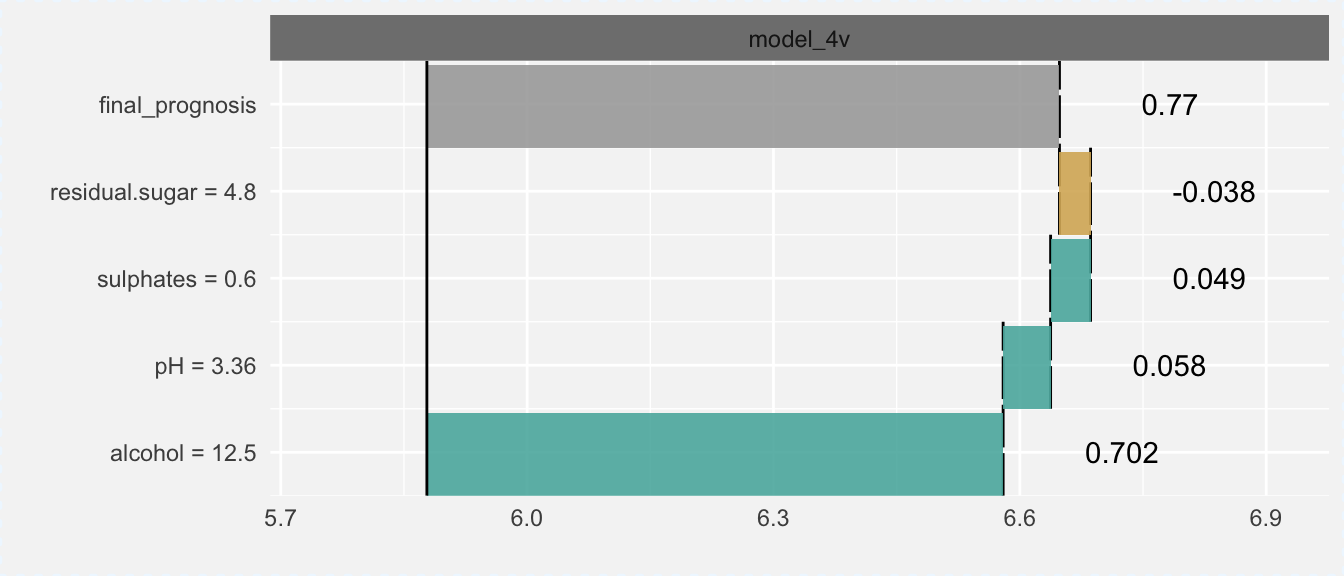
\includegraphics{DALEX_files/figure-latex/unnamed-chunk-38-1.pdf}

\subsection{Model Comparisons}\label{model-comparisons-1}

What if we have two or larger number of models? Not a problem for DALEX!

Let's fit a model with 3 variables.

\begin{Shaded}
\begin{Highlighting}[]
\KeywordTok{library}\NormalTok{(}\StringTok{"breakDown"}\NormalTok{)}
\KeywordTok{library}\NormalTok{(}\StringTok{"DALEX"}\NormalTok{)}
\NormalTok{new.wine <-}\StringTok{ }\KeywordTok{data.frame}\NormalTok{(}\DataTypeTok{citric.acid =} \FloatTok{0.35}\NormalTok{,}
                       \DataTypeTok{sulphates =} \FloatTok{0.6}\NormalTok{,}
                       \DataTypeTok{alcohol =} \FloatTok{12.5}\NormalTok{,}
                       \DataTypeTok{pH =} \FloatTok{3.36}\NormalTok{,}
                       \DataTypeTok{residual.sugar =} \FloatTok{4.8}\NormalTok{)}

\NormalTok{wine_lm_model3 <-}\StringTok{ }\KeywordTok{lm}\NormalTok{(quality }\OperatorTok{~}\StringTok{ }\NormalTok{citric.acid }\OperatorTok{+}\StringTok{  }\NormalTok{sulphates }\OperatorTok{+}\StringTok{ }\NormalTok{alcohol,}
                     \DataTypeTok{data =}\NormalTok{ wine)}
\NormalTok{wine_lm_explainer3 <-}\StringTok{ }\KeywordTok{explain}\NormalTok{(wine_lm_model3, }\DataTypeTok{data =}\NormalTok{ wine, }\DataTypeTok{label =} \StringTok{"model_3v"}\NormalTok{)}

\NormalTok{wine_lm_predict3 <-}\StringTok{ }\KeywordTok{single_prediction}\NormalTok{(wine_lm_explainer3, }\DataTypeTok{observation =}\NormalTok{ new.wine)}
\KeywordTok{plot}\NormalTok{(wine_lm_predict3)}
\end{Highlighting}
\end{Shaded}

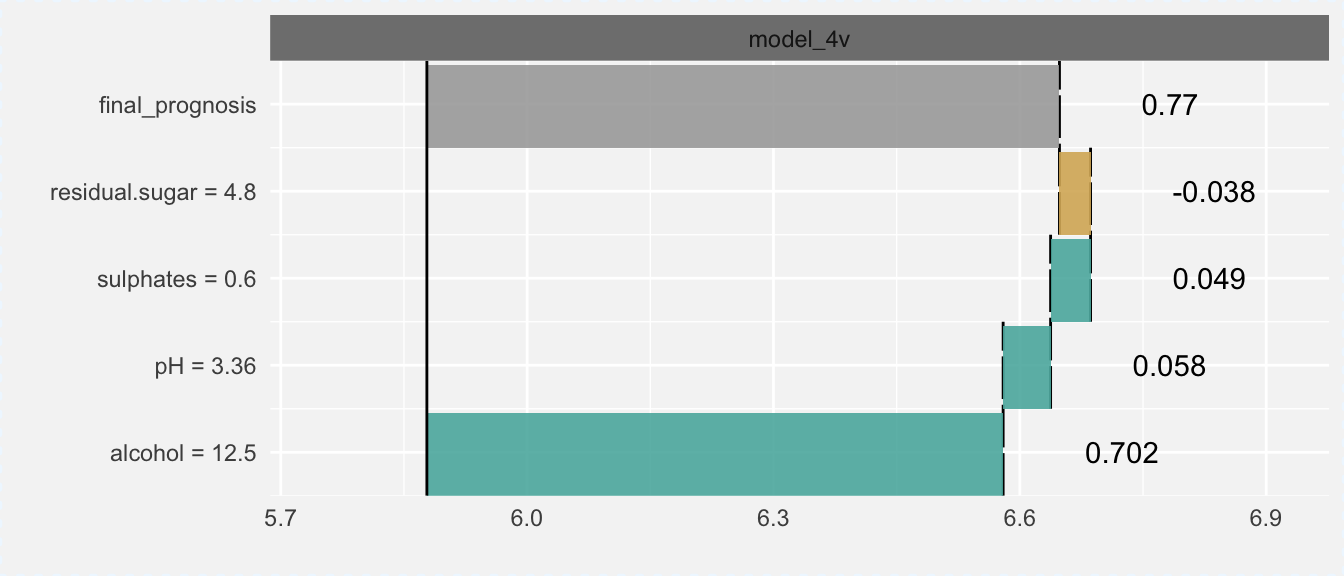
\includegraphics{DALEX_files/figure-latex/unnamed-chunk-39-1.pdf}

Let's fit a second model with 4 variables.

\begin{Shaded}
\begin{Highlighting}[]
\NormalTok{wine_lm_model4 <-}\StringTok{ }\KeywordTok{lm}\NormalTok{(quality }\OperatorTok{~}\StringTok{ }\NormalTok{pH }\OperatorTok{+}\StringTok{ }\NormalTok{residual.sugar }\OperatorTok{+}\StringTok{ }\NormalTok{sulphates }\OperatorTok{+}\StringTok{ }\NormalTok{alcohol,}
                     \DataTypeTok{data =}\NormalTok{ wine)}
\NormalTok{wine_lm_explainer4 <-}\StringTok{ }\KeywordTok{explain}\NormalTok{(wine_lm_model4, }\DataTypeTok{data =}\NormalTok{ wine, }\DataTypeTok{label =} \StringTok{"model_4v"}\NormalTok{)}

\NormalTok{wine_lm_predict4 <-}\StringTok{ }\KeywordTok{single_prediction}\NormalTok{(wine_lm_explainer4, }\DataTypeTok{observation =}\NormalTok{ new.wine)}
\KeywordTok{plot}\NormalTok{(wine_lm_predict4)}
\end{Highlighting}
\end{Shaded}

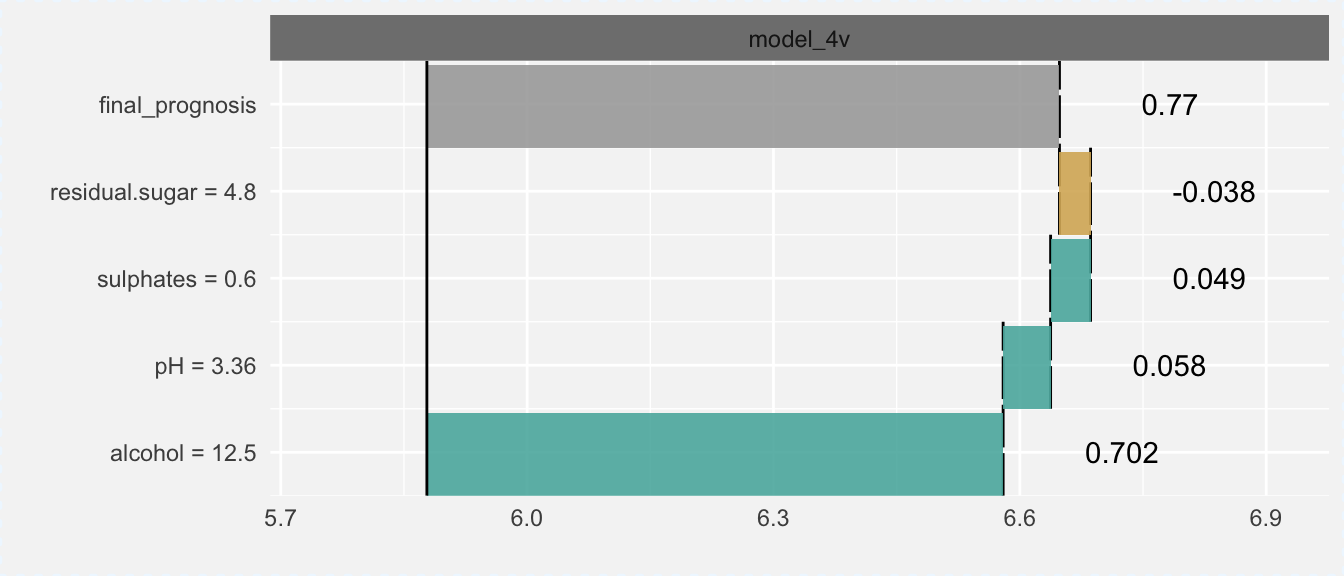
\includegraphics{DALEX_files/figure-latex/unnamed-chunk-40-1.pdf}

It's easy to compare these models. Just plot both together side by side.

\begin{Shaded}
\begin{Highlighting}[]
\KeywordTok{plot}\NormalTok{(wine_lm_predict3, wine_lm_predict4)}
\end{Highlighting}
\end{Shaded}

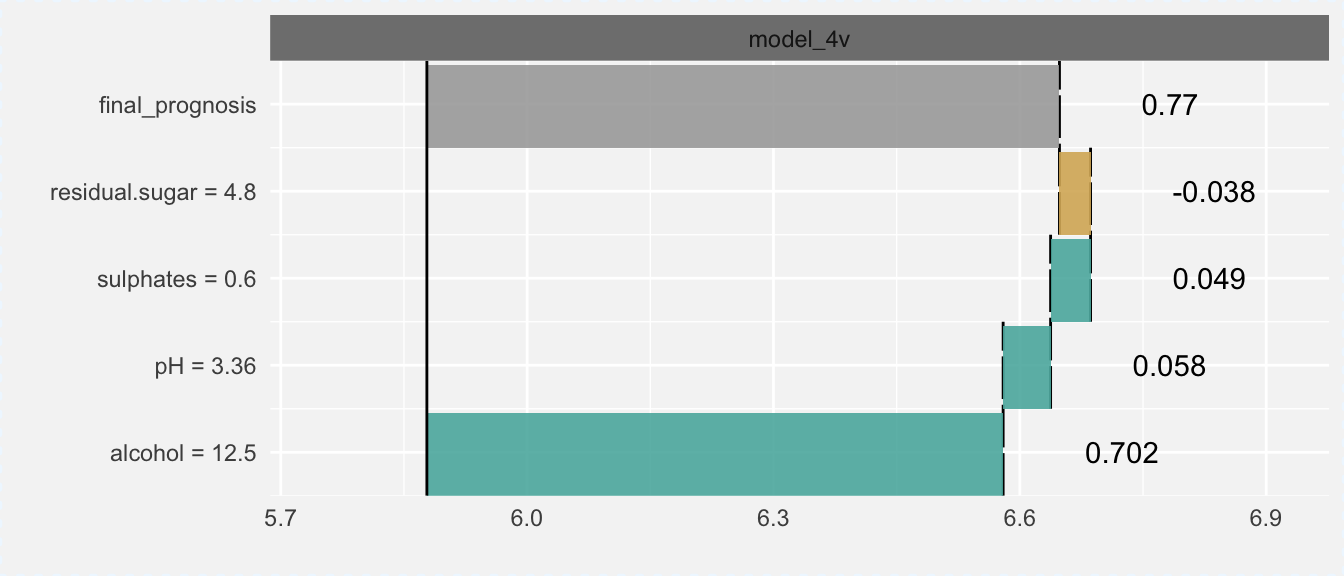
\includegraphics{DALEX_files/figure-latex/unnamed-chunk-41-1.pdf}

You can do this even for non linear models.

\begin{Shaded}
\begin{Highlighting}[]
\KeywordTok{library}\NormalTok{(}\StringTok{"randomForest"}\NormalTok{)}
\NormalTok{wine_rf_model4 <-}\StringTok{ }\KeywordTok{randomForest}\NormalTok{(quality }\OperatorTok{~}\StringTok{ }\NormalTok{pH }\OperatorTok{+}\StringTok{ }\NormalTok{residual.sugar }\OperatorTok{+}\StringTok{ }\NormalTok{sulphates }\OperatorTok{+}\StringTok{ }\NormalTok{alcohol, }\DataTypeTok{data =}\NormalTok{ wine)}
\NormalTok{wine_rf_explainer4 <-}\StringTok{ }\KeywordTok{explain}\NormalTok{(wine_rf_model4, }\DataTypeTok{data =}\NormalTok{ wine, }\DataTypeTok{label =} \StringTok{"model_rf"}\NormalTok{)}

\NormalTok{wine_rf_predict4 <-}\StringTok{ }\KeywordTok{single_prediction}\NormalTok{(wine_rf_explainer4, }\DataTypeTok{observation =}\NormalTok{ new.wine)}
\KeywordTok{plot}\NormalTok{(wine_rf_predict4, wine_lm_predict4, wine_lm_predict3)}
\end{Highlighting}
\end{Shaded}

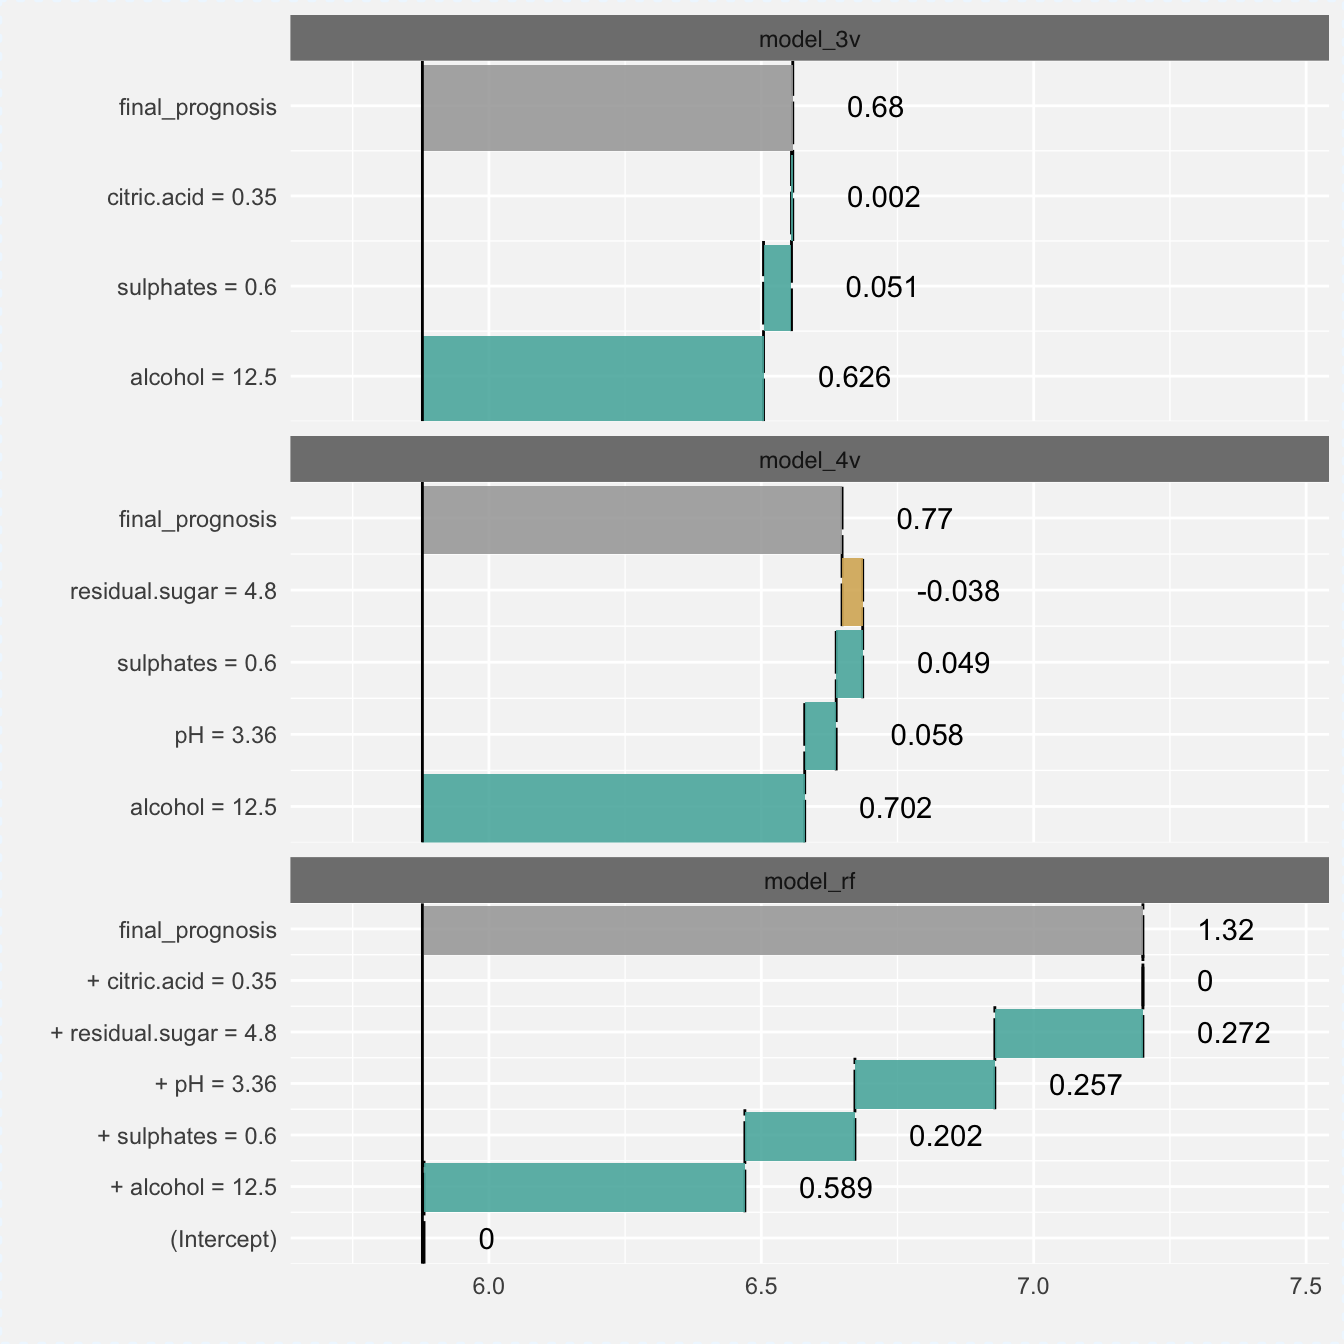
\includegraphics{DALEX_files/figure-latex/unnamed-chunk-42-1.pdf}

\chapter{Model performance}\label{model-performance}

\section{ROC}\label{roc}

\section{Lift curve}\label{lift-curve}

\chapter{Goodness of fit / Model
diagnostic}\label{goodness-of-fit-model-diagnostic}

\section{halfnorm plot}\label{halfnorm-plot}

\chapter{Reproducibility}\label{reproducibility}

Packages are changing quite fast, especially in actively developed
areas. Below you will find list of packages that were installed on my
computer when I was preparing this documentation.

It is likely that some of described packages will change names of
functions or arguments or structure of results. Use the version listed
below to reproduce results form this book.

Note, that results, models and plots created in are were recorded with
the \textbf{archivist} package \citep{archivist}. Use archivist links to
retrieve their binary copies directly to your R console.

\begin{Shaded}
\begin{Highlighting}[]
\NormalTok{devtools}\OperatorTok{::}\KeywordTok{session_info}\NormalTok{()}
\end{Highlighting}
\end{Shaded}

\begin{verbatim}
##  setting  value                       
##  version  R version 3.4.3 (2017-11-30)
##  system   x86_64, darwin15.6.0        
##  ui       X11                         
##  language (EN)                        
##  collate  en_US.UTF-8                 
##  tz       Asia/Singapore              
##  date     2018-02-21                  
## 
##  package      * version  date       source                                
##  abind          1.4-5    2016-07-21 cran (@1.4-5)                         
##  agricolae      1.2-8    2017-09-12 cran (@1.2-8)                         
##  ALEPlot        1.0      2017-11-13 CRAN (R 3.4.2)                        
##  AlgDesign      1.1-7.3  2014-10-15 CRAN (R 3.2.0)                        
##  arm            1.9-3    2016-11-27 CRAN (R 3.4.0)                        
##  assertthat     0.2.0    2017-04-11 CRAN (R 3.4.0)                        
##  backports      1.1.1    2017-09-25 CRAN (R 3.4.2)                        
##  base         * 3.4.3    2017-12-07 local                                 
##  bayesplot      1.4.0    2017-09-12 CRAN (R 3.4.3)                        
##  BBmisc         1.11     2017-03-10 cran (@1.11)                          
##  bindr          0.1      2016-11-13 CRAN (R 3.4.0)                        
##  bindrcpp     * 0.2      2017-06-17 CRAN (R 3.4.0)                        
##  blme           1.0-4    2015-06-14 CRAN (R 3.4.0)                        
##  bookdown       0.5      2017-08-20 CRAN (R 3.4.1)                        
##  boot           1.3-20   2017-08-06 CRAN (R 3.4.3)                        
##  breakDown    * 0.1.4    2018-02-17 local                                 
##  broom          0.4.2    2017-02-13 CRAN (R 3.4.0)                        
##  carData        3.0-0    2017-08-28 CRAN (R 3.4.1)                        
##  checkmate      1.8.4    2017-09-25 cran (@1.8.4)                         
##  cli            1.0.0    2017-11-05 cran (@1.0.0)                         
##  cluster        2.0.6    2017-03-10 CRAN (R 3.4.3)                        
##  coda           0.19-1   2016-12-08 cran (@0.19-1)                        
##  codetools      0.2-15   2016-10-05 CRAN (R 3.4.3)                        
##  coin           1.2-2    2017-11-28 cran (@1.2-2)                         
##  colorspace     1.3-2    2016-12-14 CRAN (R 3.4.0)                        
##  combinat       0.0-8    2012-10-29 CRAN (R 3.1.0)                        
##  compiler       3.4.3    2017-12-07 local                                 
##  cowplot        0.9.1    2017-11-16 cran (@0.9.1)                         
##  crayon         1.3.4    2017-09-16 CRAN (R 3.4.1)                        
##  DALEX        * 0.1.1    2018-02-21 local                                 
##  data.table     1.10.4-3 2017-10-27 CRAN (R 3.4.2)                        
##  datasets     * 3.4.3    2017-12-07 local                                 
##  deldir         0.1-14   2017-04-22 cran (@0.1-14)                        
##  devtools       1.13.3   2017-08-02 CRAN (R 3.4.1)                        
##  digest         0.6.15   2018-01-28 cran (@0.6.15)                        
##  dplyr          0.7.4    2017-09-28 CRAN (R 3.4.2)                        
##  DT             0.1      2015-06-09 CRAN (R 3.2.0)                        
##  effects        4.0-0    2017-09-15 CRAN (R 3.4.1)                        
##  evaluate       0.10.1   2017-06-24 CRAN (R 3.4.1)                        
##  expm           0.999-2  2017-03-29 cran (@0.999-2)                       
##  factorMerger * 0.3.5    2018-01-11 local (geneticsMiNIng/FactorMerger@NA)
##  forcats        0.2.0    2017-01-23 CRAN (R 3.4.0)                        
##  foreign        0.8-69   2017-06-22 CRAN (R 3.4.3)                        
##  forestmodel  * 0.4.3    2017-04-16 CRAN (R 3.4.0)                        
##  gdata          2.17.0   2015-07-04 CRAN (R 3.2.0)                        
##  ggeffects      0.3.0    2017-11-27 CRAN (R 3.4.3)                        
##  ggplot2      * 2.2.1    2016-12-30 CRAN (R 3.4.0)                        
##  ggpubr         0.1.6    2017-11-14 cran (@0.1.6)                         
##  glmmTMB        0.2.0    2017-12-11 CRAN (R 3.4.3)                        
##  glue           1.1.1    2017-06-21 CRAN (R 3.4.1)                        
##  gmodels        2.16.2   2015-07-22 CRAN (R 3.4.0)                        
##  graphics     * 3.4.3    2017-12-07 local                                 
##  grDevices    * 3.4.3    2017-12-07 local                                 
##  grid           3.4.3    2017-12-07 local                                 
##  gridExtra      2.3      2017-09-09 CRAN (R 3.4.1)                        
##  gtable         0.2.0    2016-02-26 CRAN (R 3.2.3)                        
##  gtools         3.5.0    2015-05-29 CRAN (R 3.2.0)                        
##  haven          1.1.0    2017-07-09 CRAN (R 3.4.1)                        
##  highr          0.6      2016-05-09 CRAN (R 3.4.0)                        
##  htmltools      0.3.6    2017-04-28 CRAN (R 3.4.0)                        
##  htmlwidgets    0.9      2017-07-10 CRAN (R 3.4.1)                        
##  httpuv         1.3.5    2017-07-04 CRAN (R 3.4.1)                        
##  ICEbox       * 1.1.2    2017-07-13 CRAN (R 3.4.1)                        
##  klaR           0.6-12   2014-08-06 CRAN (R 3.2.0)                        
##  knitr          1.18     2017-12-27 cran (@1.18)                          
##  labeling       0.3      2014-08-23 CRAN (R 3.2.2)                        
##  lattice        0.20-35  2017-03-25 CRAN (R 3.4.3)                        
##  lazyeval       0.2.0    2016-06-12 CRAN (R 3.4.0)                        
##  LearnBayes     2.15     2014-05-29 CRAN (R 3.2.0)                        
##  live         * 1.3.2    2018-01-25 local (MI2DataLab/live@f38ef48)       
##  lme4           1.1-15   2017-12-21 cran (@1.1-15)                        
##  lmtest         0.9-34   2015-06-06 CRAN (R 3.2.0)                        
##  lubridate      1.7.2    2018-02-06 cran (@1.7.2)                         
##  magrittr       1.5      2014-11-22 CRAN (R 3.2.2)                        
##  MASS           7.3-47   2017-02-26 CRAN (R 3.4.3)                        
##  Matrix         1.2-12   2017-11-15 CRAN (R 3.4.2)                        
##  memoise        1.1.0    2017-04-21 CRAN (R 3.4.0)                        
##  merTools       0.3.0    2016-12-12 CRAN (R 3.4.0)                        
##  methods      * 3.4.3    2017-12-07 local                                 
##  mime           0.5      2016-07-07 CRAN (R 3.4.0)                        
##  minqa          1.2.4    2014-10-09 CRAN (R 3.1.1)                        
##  mlr          * 2.11     2017-03-15 cran (@2.11)                          
##  mnormt         1.5-5    2016-10-15 CRAN (R 3.4.0)                        
##  modelr         0.1.1    2017-07-24 CRAN (R 3.4.1)                        
##  modeltools     0.2-21   2013-09-02 CRAN (R 3.1.2)                        
##  multcomp       1.4-8    2017-11-08 cran (@1.4-8)                         
##  munsell        0.4.3    2016-02-13 CRAN (R 3.2.3)                        
##  mvtnorm        1.0-6    2017-03-02 CRAN (R 3.4.0)                        
##  nlme           3.1-131  2017-02-06 CRAN (R 3.4.3)                        
##  nloptr         1.0.4    2014-08-04 CRAN (R 3.2.2)                        
##  nnet           7.3-12   2016-02-02 CRAN (R 3.4.3)                        
##  parallel       3.4.3    2017-12-07 local                                 
##  parallelMap    1.3      2015-06-10 cran (@1.3)                           
##  ParamHelpers * 1.10     2017-01-05 cran (@1.10)                          
##  pdp          * 0.6.0    2017-07-20 CRAN (R 3.4.1)                        
##  pillar         1.1.0    2018-01-14 cran (@1.1.0)                         
##  pkgconfig      2.0.1    2017-03-21 CRAN (R 3.4.0)                        
##  plyr           1.8.4    2016-06-08 CRAN (R 3.4.0)                        
##  prediction     0.2.0    2017-04-19 CRAN (R 3.4.0)                        
##  proxy          0.4-20   2017-12-12 cran (@0.4-20)                        
##  psych          1.7.3.21 2017-03-22 CRAN (R 3.4.0)                        
##  purrr          0.2.4    2017-10-18 cran (@0.2.4)                         
##  pwr            1.2-1    2017-03-25 CRAN (R 3.4.0)                        
##  R6             2.2.2    2017-06-17 CRAN (R 3.4.0)                        
##  randomForest * 4.6-12   2015-10-07 CRAN (R 3.2.0)                        
##  RColorBrewer   1.1-2    2014-12-07 CRAN (R 3.2.2)                        
##  Rcpp           0.12.15  2018-01-20 cran (@0.12.15)                       
##  reshape2       1.4.3    2017-12-11 cran (@1.4.3)                         
##  rlang          0.1.6    2017-12-21 CRAN (R 3.4.3)                        
##  rmarkdown      1.8      2017-11-17 cran (@1.8)                           
##  rprojroot      1.2      2017-01-16 CRAN (R 3.4.0)                        
##  rstudioapi     0.7      2017-09-07 CRAN (R 3.4.1)                        
##  sandwich       2.4-0    2017-07-26 cran (@2.4-0)                         
##  scales         0.5.0    2017-08-24 CRAN (R 3.4.1)                        
##  sfsmisc      * 1.1-1    2017-06-08 CRAN (R 3.4.0)                        
##  shiny          1.0.5    2017-08-23 CRAN (R 3.4.1)                        
##  sjlabelled     1.0.5    2017-11-09 CRAN (R 3.4.2)                        
##  sjmisc         2.6.3    2017-11-28 CRAN (R 3.4.3)                        
##  sjPlot       * 2.4.0    2017-10-19 CRAN (R 3.4.2)                        
##  sjstats        0.13.0   2017-11-23 CRAN (R 3.4.3)                        
##  snakecase      0.5.1    2017-09-20 CRAN (R 3.4.2)                        
##  sp             1.2-5    2017-06-29 cran (@1.2-5)                         
##  spData         0.2.6.4  2017-11-12 cran (@0.2.6.4)                       
##  spdep          0.7-4    2017-11-22 cran (@0.7-4)                         
##  splines        3.4.3    2017-12-07 local                                 
##  stats        * 3.4.3    2017-12-07 local                                 
##  stats4         3.4.3    2017-12-07 local                                 
##  stringdist     0.9.4.1  2016-01-02 CRAN (R 3.2.3)                        
##  stringi        1.1.6    2017-11-17 cran (@1.1.6)                         
##  stringr        1.2.0    2017-02-18 CRAN (R 3.4.0)                        
##  survey         3.30-3   2014-08-15 CRAN (R 3.1.2)                        
##  survival       2.41-3   2017-04-04 CRAN (R 3.4.3)                        
##  TH.data        1.0-8    2017-01-23 cran (@1.0-8)                         
##  tibble         1.4.2    2018-01-22 cran (@1.4.2)                         
##  tidyr          0.7.2    2017-10-16 cran (@0.7.2)                         
##  tidyselect     0.2.2    2017-10-10 cran (@0.2.2)                         
##  TMB            1.7.12   2017-12-11 CRAN (R 3.4.3)                        
##  tools          3.4.3    2017-12-07 local                                 
##  tufte          0.2      2016-02-07 CRAN (R 3.4.0)                        
##  utils        * 3.4.3    2017-12-07 local                                 
##  withr          2.1.0    2017-11-01 cran (@2.1.0)                         
##  xgboost      * 0.6-4    2017-01-05 cran (@0.6-4)                         
##  xtable         1.8-2    2016-02-05 CRAN (R 3.2.3)                        
##  yaImpute       1.0-29   2017-12-10 CRAN (R 3.4.3)                        
##  yaml           2.1.16   2017-12-12 cran (@2.1.16)                        
##  zoo            1.8-0    2017-04-12 CRAN (R 3.4.0)
\end{verbatim}

\chapter{Hands-on tutorial}\label{hands-on-tutorial}

\section{Title}\label{title}

DALEX: Descriptive mAchine Learning EXplanations

Tools for exploration, validation and explanation of complex machine
learning models

\section{Outline}\label{outline}

Complex machine learning models are frequently used in predictive
modelling. There are a lot of examples for random forest like or
boosting like models in medicine, finance, agriculture etc. In this
workshop we will show why and how one would analyse the structure of the
black-box model.

This will be a hands-on workshop with four parts. In each part there
will be a short lecture (around 20-25 minutes) and then time for
practice and discussion (around 20-25 min).

\begin{itemize}
\tightlist
\item
  Introduction
\end{itemize}

Here we will show what problems may arise from blind application of
black-box models. Also we will show situations in which the
understanding of a model structure leads to model improvements, model
stability and larger trust in the model.

During the hands-on part we will fit few complex models (like xgboost,
randomForest) with the mlr package and discuss basic diagnostic tools
for these models.

\begin{itemize}
\tightlist
\item
  Conditional Explainers
\end{itemize}

In this part we will introduce techniques for understanding of
marginal/conditional response of a model given a one- two- variables. We
will cover PDP (Partial Dependence Plots) and ICE (Individual
Conditional Expectations) packages for continuous variables and MPP
(Merging Path Plot from factorMerger package) for categorical variables.

\begin{itemize}
\tightlist
\item
  Local Explainers
\end{itemize}

In this part we will introduce techniques that explain key factors that
drive single model predictions. This covers Break Down plots for linear
models (lm / glm) and tree-based models (randomForestExplainer,
xgboostExplainer) along with model agnostic approaches implemented in
the live package (an extension of the LIME method).

\begin{itemize}
\tightlist
\item
  Global Explainers
\end{itemize}

In this part we will introduce tools for global analysis of the
black-box model, like variable importance plots, interaction importance
plots and tools for model diagnostic.

\begin{itemize}
\tightlist
\item
  Literature
\end{itemize}

Staniak, Mateusz, and Przemysław Biecek. 2017. Live: Local Interpretable
(Model-Agnostic) Visual Explanations.

Sitko, Agnieszka, and Przemyslaw Biecek. 2017. FactorMerger:
Hierarchical Algorithm for Post-Hoc Testing.
\url{https://github.com/MI2DataLab/factorMerger}.

Greenwell, Brandon M. 2017. ``Pdp: An R Package for Constructing Partial
Dependence Plots.'' The R Journal 9 (1): 421--36.
\url{https://journal.r-project.org/archive/2017/RJ-2017-016/index.html}.

Goldstein, Alex, Adam Kapelner, Justin Bleich, and Emil Pitkin. 2015.
``Peeking Inside the Black Box: Visualizing Statistical Learning with
Plots of Individual Conditional Expectation.'' Journal of Computational
and Graphical Statistics 24 (1): 44--65.
\url{doi:10.1080/10618600.2014.907095}.

Apley, Dan. 2017. ALEPlot: Accumulated Local Effects (Ale) Plots and
Partial Dependence (Pd) Plots.
\url{https://CRAN.R-project.org/package=ALEPlot}.

Ribeiro, Marco Tulio, Sameer Singh, and Carlos Guestrin. 2016. ``\,`Why
Should I Trust You?': Explaining the Predictions of Any Classifier.''
In, 1135--44. ACM Press. \url{doi:10.1145/2939672.2939778}.

Biecek, Przemyslaw. 2017. BreakDown: BreakDown Plots.
\url{https://CRAN.R-project.org/package=breakDown}.

\section{Keywords}\label{keywords}

machine learning, black-box model, model explainers, model auditing,
model visualization

\section{Equipment}\label{equipment}

Laptop with preinstalled R and selected packages. All necessary models
and datasets will be provided in advance.

\section{Target audience}\label{target-audience}

Applied data scientists, analysts interested in machine learning models.

\section{Motivation}\label{motivation-1}

There are at least three good reasons why this tutoial will be
interesting for conference participants.

\begin{enumerate}
\def\labelenumi{\arabic{enumi})}
\item
  The topic is super interesting. Even short blog posts on R Bloggers
  (like
  \url{http://smarterpoland.pl/index.php/2017/12/explain-explain-explain/})
  got lots of reactions. There is a large community around model
  explainer sin python (the ELI5 package) and there is growing community
  for R. I had a talk about explainers during the last UseR conference
  2017
  (\url{https://user2017.sched.com/event-goers/10415a8ff5675f10deb3fd27b43db5a7})
  more than 500 users sign for it.
\item
  We have developed consistent toolbox of R packages - called DALEX -
  that supports model explanations. Participants of the workshop will
  learn easy-to-use tools that can be applied in their every-day data
  analyses. Methods that we will describe work for most of popular ML
  models (random forest, glm, boosting).
\item
  Anything related to Machine Learning brings a lot of participants.
  I've attended ML-related workshops during UseR 2015, UseR 2016 and
  UseR 2017. Demand for such tutorials was always the highest.
\end{enumerate}

This is why we expect a high interest in this tutorial.

\bibliography{book.bib,packages.bib}


\end{document}
